\documentclass[journal=jcisd8,manuscript=article]{achemso}

% ===== Packages =====
\usepackage{amsmath,amssymb,amsfonts}
\usepackage{graphicx}
\usepackage{booktabs}
\usepackage{subcaption}
\usepackage{siunitx}
\usepackage{adjustbox}
\usepackage{soul}
\usepackage{tikz}
\usetikzlibrary{arrows.meta, positioning, shapes, calc, fit, decorations.pathreplacing}
\usepackage{longtable}
\usepackage{multirow}
\usepackage[dvipsnames]{xcolor}
\usepackage{colortbl}
\usepackage{placeins}

% ===== Custom Commands =====
\newcommand{\vect}[1]{\mathbf{#1}}
\newcommand{\matr}[1]{\mathbf{#1}}
\definecolor{goodpred}{RGB}{198,239,206}
\newcommand{\gp}[1]{\cellcolor{goodpred}{#1}}

% ===== Title and Authors =====
\title{When Do Simple Models Win? Machine Learning Architectures for UV Absorption Prediction}

\author{Umesh Arampath}
\email{uarampath@mwbioprocessing.com}
\affiliation{Department of Mathematics, University of Iowa, Iowa City, USA}
\alsoaffiliation{Midwest Bioprocessing Center, Illinois, USA}

\author{Bryant Pero}
\affiliation{Midwest Bioprocessing Center, Illinois, USA}

\author{David Stewart}
\affiliation{Department of Mathematics, University of Iowa, Iowa City, USA}

\author{David Demirjian}
\affiliation{Midwest Bioprocessing Center, Illinois, USA}

\keywords{UV absorption, molecular property prediction, deep learning, random forest, Morgan fingerprints, graph neural network, directed message passing, pretrained Transformer, solvent effects, benchmarking}

\begin{document}

\maketitle

% ===== Abstract =====
\begin{abstract}
What determines which machine learning architecture wins for molecular property prediction?
We address this question through a controlled comparison of five models spanning four architecture families: fingerprint-based ensembles (Random Forest, XGBoost), a directed message-passing graph neural network (GNN), a bidirectional gated recurrent network (BiGRU), and a pretrained Transformer, using UV absorption wavelength ($\lambda_{\max}$) prediction as a testbed across 18,755 solute--solvent pairs with stratified 5-fold cross-validation and two external datasets totaling over 40,000 molecules.
The answer depends on the task.
For screening within known chemical space, RF with Morgan fingerprints is competitive with the best deep learning model at a fraction of the compute cost: RF and the D-MPNN are statistically indistinguishable (RMSE = $31.34 \pm 1.82$ vs.\ $31.69 \pm 3.18$~nm, $p = 0.77$), and RF trains in 15 minutes on a CPU with no hyperparameter tuning while outperforming all sequence-based models.
For exploring novel scaffolds, deep learning is superior: experimental validation on 16 novel UV-absorbing compounds shows that the GNN (MAE = 26.2~nm), Transformer (26.3~nm), and BiGRU (28.6~nm) all outperform RF (38.5~nm), as learned representations generalize where fixed fingerprints cannot.
In either case, encoding solvent identity improves all models: a simple SMILES/fingerprint concatenation strategy yields 6--8\% RMSE reductions across fingerprint, graph, and recurrent architectures ($p < 0.02$), without domain-specific descriptor engineering.
Interpretability analysis confirms that both RF feature importance and BiGRU gradient saliency independently highlight the same chromophore motifs, and that architectures with local inductive bias systematically outperform global-attention Transformers on this locally determined property.
Within UV absorption prediction, optimal model choice depends on the relationship between target compounds and available training data: simple fingerprint-based models are an efficient and accurate alternative to deep learning for interpolation within known chemical space, while learned representations from graphs, sequences, or pretraining generalize better to novel scaffolds. We further hypothesize that this pattern---local-bias architectures favored for properties governed by local molecular features---may extend to other locally determined molecular properties; validating this across property types is left as future work.
\end{abstract}

% ===== Introduction =====
\section{Introduction}
\label{sec:introduction}

Ultraviolet--visible (UV--Vis) absorption is a fundamental property of many chemicals, with the wavelength of maximum absorption ($\lambda_{\max}$) serving as a key property for molecular characterization, photosafety assessment, and materials design~\cite{flemingMolecular2010}.
When a molecule absorbs UV--Vis light, electrons undergo transitions between molecular orbitals; $\lambda_{\max}$ corresponds to the most probable electronic transition and is governed by the extent of $\pi$-conjugation, heteroatom substituents, and molecular geometry~\cite{reichardt2011solvents}.
Experimental determination of $\lambda_{\max}$ requires synthesizing and measuring each compound, creating a demand for accurate \textit{in silico} prediction methods that can accelerate screening of large chemical libraries~\cite{ghosh2019deep}.

Machine learning (ML) approaches for molecular property prediction have proliferated in recent years, spanning classical methods using engineered molecular descriptors (e.g., Morgan fingerprints~\cite{rogers2010extended} with Random Forest~\cite{breiman2001random}) to deep learning architectures that learn representations directly from molecular strings (SMILES~\cite{weininger1988smiles}) or graphs~\cite{gilmer2017neural}.
Large curated datasets such as the Joung+Beard database~\cite{joung2020experimental, beard2019comparative} and benchmarking suites like MoleculeNet~\cite{wuMoleculeNet2018} have accelerated progress, yet systematic comparisons across multiple datasets with consistent methodology remain rare. Without such comparisons, practitioners lack guidance on which model families to deploy for a given chemistry domain.
Recent work has highlighted that well-tuned classical models can match or exceed complex deep learning architectures for molecular property prediction~\cite{panapitiya2022evaluation, walters2021applications, fooladi2025evaluating}, suggesting that no universal ``best model'' exists; rather, the optimal choice depends on the interplay between molecular representation, property type, and the novelty of target compounds relative to training data.

The UV absorption prediction task is well-suited for systematic architecture comparison for several reasons:
\begin{enumerate}
    \item \textbf{Solvent dependence:} $\lambda_{\max}$ varies with solvent environment (solvatochromism), requiring models to encode both solute structure and solvent identity.
    \item \textbf{Representation diversity:} Although absorption fundamentally depends on electronic structure influenced by molecular geometry, our results show that 1D and 2D representations (Morgan fingerprints, SMILES strings, molecular graphs) capture the dominant structure--property relationships for UV absorption without requiring explicit 3D coordinates. Methods that incorporate 3D conformational information are not evaluated in this work and are discussed in the Limitations and Future Work sections.
    \item \textbf{Diverse benchmarks:} Multiple published datasets with varying sizes, chemical spaces, and evaluation protocols enable comprehensive assessment.
    \item \textbf{Practical relevance:} ICH~S10 guidelines require photosafety screening of pharmaceutical compounds, where $\lambda_{\max}$ prediction serves as a first-pass filter.
\end{enumerate}

In this work, we present a study comparing five ML models spanning four architecture families---fingerprint-based ensembles (Random Forest, XGBoost), a directed message-passing graph neural network (D-MPNN), a bidirectional gated recurrent network (BiGRU), and a pretrained Transformer---for $\lambda_{\max}$ prediction.
Our key contributions are:
\begin{itemize}
    \item \textbf{Practical model selection guidance:} on in-distribution screening, RF is statistically tied with the best deep learning model (D-MPNN, $p = 0.77$) but trains $\sim$100$\times$ faster with no hyperparameter tuning; on novel compounds, deep learning models generalize better. We validate this on 16 experimentally measured UV-absorbing molecules.
    \item \textbf{Controlled multi-architecture comparison} across three datasets using published evaluation protocols. The D-MPNN with default hyperparameters sets new state-of-the-art results on both external datasets, while RF and D-MPNN are statistically tied on primary cross-validation.
    \item \textbf{Optimized BiGRU architecture} via Bayesian hyperparameter search (3-layer, 256-unit, 4.8\% RMSE improvement), demonstrating that a sequence-based approach operating on raw SMILES can match graph and fingerprint methods without compromising prediction accuracy.
    \item \textbf{Concatenation-based solvent encoding generalizes across architectures:} the same strategy of concatenating native solute and solvent representations---Morgan fingerprints for the tree ensembles, SMILES strings for the sequence models, and molecular graphs for the D-MPNN---yields 6--8\% RMSE reductions across all three architecture families ($p < 0.02$), without domain-specific descriptor engineering.
    \item \textbf{Locality-of-property hypothesis:} architectures with local inductive bias systematically outperform global-attention Transformers on UV absorption, which is determined by local electronic structure~\cite{chenMolecularLanguage2023}. All three encode molecular structure with an implicit spatial cutoff (Morgan fingerprints through a fixed radius, D-MPNN through bounded message-passing depth, and BiGRU through gradient decay in the recurrent hidden state), while Transformers impose no such locality constraint through global self-attention. RF feature importance and BiGRU gradient saliency independently highlight the same chromophore motifs, confirming that both architectures learn meaningful photochemistry.
    \item \textbf{Photosafety application:} ICH~S10 classification on a reconstructed Reaxys dataset validates practical utility.
\end{itemize}

The choice of molecular representation fundamentally determines which ML methods can be applied.
SMILES (Simplified Molecular Input Line Entry System)~\cite{weininger1988smiles} encodes molecular graphs as character strings, enabling NLP-inspired sequence models (RNNs, Transformers), while Morgan circular fingerprints~\cite{rogers2010extended} encode local chemical environments as fixed-length binary vectors amenable to classical tree-based ensembles~\cite{landrum2016rdkit, wuMoleculeNet2018}.
Our benchmark compares three representation families: fingerprint-based models (RF, XGBoost), a graph neural network (Chemprop D-MPNN), and sequence-based models (BiGRU, ChemBERTa) on the same prediction task.
Figure~\ref{fig:benchmark_framework} provides an overview of this multi-pathway framework.

\begin{figure}[!ht]
    \centering
    % ===== (a) Input and Representation =====
    \begin{subfigure}[b]{\textwidth}
    \centering
    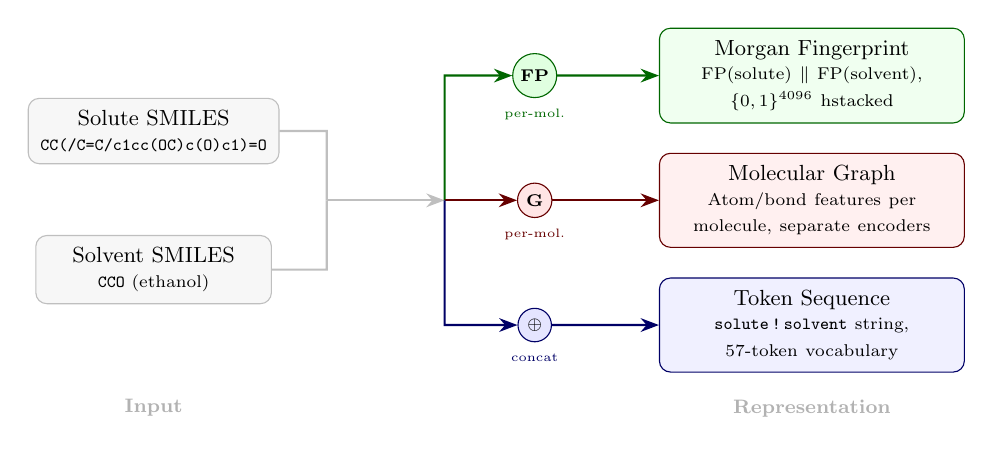
\begin{tikzpicture}[scale=0.88, every node/.style={scale=0.88},
        >=Stealth,
        box/.style={draw, rounded corners=4pt, align=center, font=\small, inner sep=5pt},
        arr/.style={->, thick, draw=gray!50},
    ]
    % ---- Input boxes (identical size) ----
    \node[box, fill=gray!6, draw=gray!50, minimum width=3.4cm] (mol) at (0, 1.0)
        {Solute SMILES\\[-1pt]{\scriptsize\texttt{CC(/C=C/c1cc(OC)c(O)c1)=O}}};
    \node[box, fill=gray!6, draw=gray!50, minimum width=3.4cm] (solv) at (0, -1.0)
        {Solvent SMILES\\[-1pt]{\scriptsize\texttt{CCO} (ethanol)}};

    % ---- Input arrows: two lines join into one arrow ----
    \draw[thick, draw=gray!50] (mol.east) -- (2.5, 1.0) -- (2.5, 0);
    \draw[thick, draw=gray!50] (solv.east) -- (2.5, -1.0) -- (2.5, 0);
    % Single arrow from join point to fork
    \coordinate (fork) at (4.2, 0);
    \draw[arr] (2.5, 0) -- (fork);

    % ---- Green path (top): independent FPs, then hstacked ----
    \node[draw, circle, fill=green!12, draw=green!40!black, inner sep=2pt,
          font=\scriptsize\bfseries] (fpnode) at (5.5, 1.8) {FP};
    \node[font=\tiny, green!40!black, below=1pt of fpnode] {per-mol.};

    \node[box, fill=green!6, draw=green!40!black, minimum width=4.4cm, text width=4.0cm] (fp) at (9.5, 1.8)
        {Morgan Fingerprint\\[-1pt]{\scriptsize FP(solute) $\|$ FP(solvent), $\{0,1\}^{4096}$ hstacked}};

    \draw[arr, draw=green!40!black] (fork) -- (4.2, 1.8) -- (fpnode);
    \draw[arr, draw=green!40!black] (fpnode) -- (fp.west);

    % ---- Red path (middle): molecular graph ----
    \node[draw, circle, fill=red!10, draw=red!40!black, inner sep=2pt,
          font=\scriptsize\bfseries] (graphnode) at (5.5, 0) {G};
    \node[font=\tiny, red!40!black, below=1pt of graphnode] {per-mol.};

    \node[box, fill=red!6, draw=red!40!black, minimum width=4.4cm, text width=4.0cm] (mg) at (9.5, 0)
        {Molecular Graph\\[-1pt]{\scriptsize Atom/bond features per molecule, separate encoders}};

    \draw[arr, draw=red!40!black] (fork) -- (4.2, 0) -- (graphnode);
    \draw[arr, draw=red!40!black] (graphnode) -- (mg.west);

    % ---- Blue path (bottom): SMILES concat, then tokenized ----
    \node[draw, circle, fill=blue!10, draw=blue!40!black, inner sep=2pt,
          font=\scriptsize\bfseries] (cat) at (5.5, -1.8) {$\oplus$};
    \node[font=\tiny, blue!40!black, below=1pt of cat] {concat};

    \node[box, fill=blue!6, draw=blue!40!black, minimum width=4.4cm, text width=4.0cm] (seq) at (9.5, -1.8)
        {Token Sequence\\[-1pt]{\scriptsize \texttt{solute\,!\,solvent} string, 57-token vocabulary}};

    \draw[arr, draw=blue!40!black] (fork) -- (4.2, -1.8) -- (cat);
    \draw[arr, draw=blue!40!black] (cat) -- (seq.west);

    % ---- Stage labels ----
    \node[font=\footnotesize\bfseries, gray!60] at (0, -3.0) {\textsc{Input}};
    \node[font=\footnotesize\bfseries, gray!60] at (9.5, -3.0) {\textsc{Representation}};

    \end{tikzpicture}
    \caption{Input and representation. Both solute and solvent SMILES feed three pathways. The fingerprint path (green) computes Morgan FPs independently per molecule and hstacks them (2048+2048 = 4096-bit). The graph path (red) converts each SMILES to a molecular graph with atom and bond features. The sequence path (blue) concatenates the SMILES strings before tokenization.}
    \label{fig:framework_input}
    \end{subfigure}

    \vspace{0.3cm}

    % ===== (b) Models and Prediction =====
    \begin{subfigure}[b]{\textwidth}
    \centering
    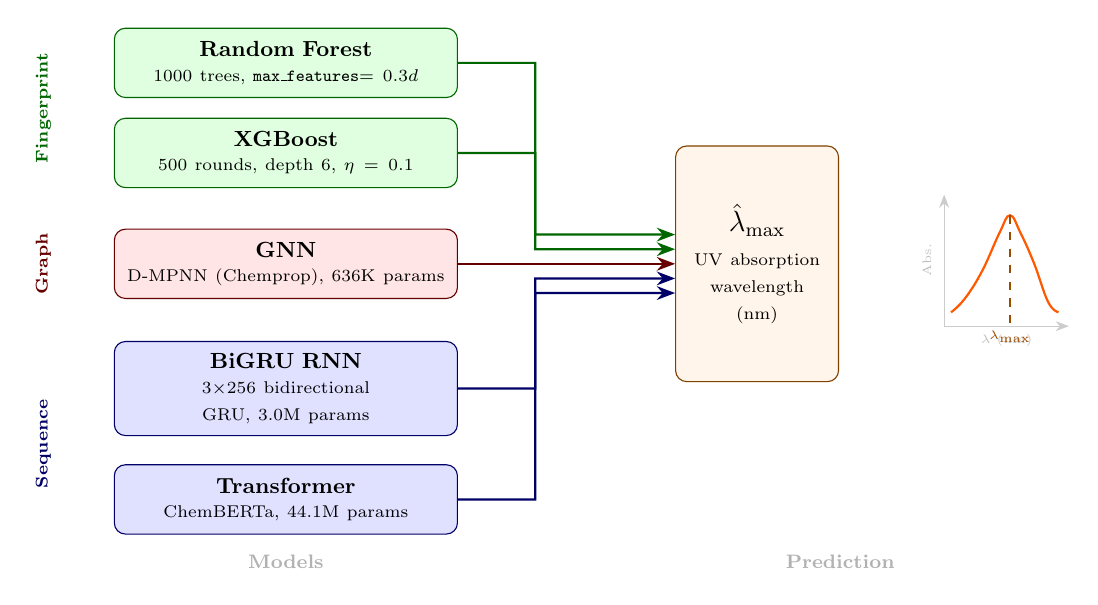
\begin{tikzpicture}[scale=0.88, every node/.style={scale=0.88},
        >=Stealth,
        box/.style={draw, rounded corners=4pt, align=center, font=\small,
                     inner sep=5pt, text width=4.6cm, minimum height=1.0cm},
        arr/.style={->, thick},
    ]

    % ---- Five models, equal spacing, grouped by color ----
    \node[box, fill=green!12, draw=green!40!black] (rf) at (0, 2.9)
        {\textbf{Random Forest}\\[-1pt]{\scriptsize 1000 trees, \texttt{max\_features}$= 0.3d$}};

    \node[box, fill=green!12, draw=green!40!black] (xgb) at (0, 1.6)
        {\textbf{XGBoost}\\[-1pt]{\scriptsize 500 rounds, depth 6, $\eta = 0.1$}};

    \node[box, fill=red!10, draw=red!40!black] (chemprop) at (0, 0)
        {\textbf{GNN}\\[-1pt]{\scriptsize D-MPNN (Chemprop), 636K params}};

    \node[box, fill=blue!12, draw=blue!40!black] (bigru) at (0, -1.8)
        {\textbf{BiGRU RNN}\\[-1pt]{\scriptsize 3$\times$256 bidirectional GRU, 3.0M params}};

    \node[box, fill=blue!12, draw=blue!40!black] (cb) at (0, -3.4)
        {\textbf{Transformer}\\[-1pt]{\scriptsize ChemBERTa, 44.1M params}};

    % ---- Group labels (rotated, centered on each group) ----
    \node[font=\scriptsize\bfseries, green!40!black, rotate=90, anchor=center,
          text width=, minimum height=0pt] at (-3.5, 2.25) {Fingerprint};
    \node[font=\scriptsize\bfseries, red!40!black, rotate=90, anchor=center,
          text width=, minimum height=0pt] at (-3.5, 0) {Graph};
    \node[font=\scriptsize\bfseries, blue!40!black, rotate=90, anchor=center,
          text width=, minimum height=0pt] at (-3.5, -2.6) {Sequence};

    % ---- Output box ----
    \node[box, fill=orange!8, draw=orange!50!black, text width=2.0cm,
          minimum height=3.4cm] (out) at (6.8, 0)
        {\textbf{\large $\hat{\lambda}_{\max}$}\\[3pt]{\scriptsize UV absorption}\\{\scriptsize wavelength (nm)}};

    % ---- Arrows: five models to output ----
    \draw[arr, draw=green!40!black] (rf.east)       -- (3.6, 2.9)   |- ([yshift=12pt]out.west);
    \draw[arr, draw=green!40!black] (xgb.east)      -- (3.6, 1.6)   |- ([yshift=6pt]out.west);
    \draw[arr, draw=red!40!black]   (chemprop.east) -- (3.6, 0)     |- (out.west);
    \draw[arr, draw=blue!40!black]  (bigru.east)    -- (3.6, -1.8)  |- ([yshift=-6pt]out.west);
    \draw[arr, draw=blue!40!black]  (cb.east)       -- (3.6, -3.4)  |- ([yshift=-12pt]out.west);

    % ---- Mini UV spectrum ----
    \begin{scope}[shift={(9.5, 0)}]
        \draw[gray!40, ->] (0,-0.9) -- (0,1.0);
        \node[font=\tiny, gray!50, rotate=90, text width=, minimum height=0pt] at (-0.25, 0.05) {Abs.};
        \draw[gray!40, ->] (0,-0.9) -- (1.8,-0.9);
        \node[font=\tiny, gray!50, text width=, minimum height=0pt] at (0.9, -1.1) {$\lambda$ (nm)};
        \draw[orange!70!red, thick, smooth, tension=0.7]
            plot coordinates {(0.1,-0.7) (0.3,-0.5) (0.55,-0.1) (0.8,0.45) (0.95,0.7) (1.1,0.45) (1.3,0.0) (1.5,-0.55) (1.65,-0.7)};
        \draw[dashed, orange!60!black] (0.95,0.7) -- (0.95,-0.9);
        \node[font=\tiny\bfseries, orange!60!black, text width=, minimum height=0pt] at (0.95, -1.05) {$\lambda_{\max}$};
    \end{scope}

    % ---- Stage labels ----
    \node[font=\footnotesize\bfseries, gray!60, text width=, minimum height=0pt] at (0, -4.3) {\textsc{Models}};
    \node[font=\footnotesize\bfseries, gray!60, text width=, minimum height=0pt] at (8.0, -4.3) {\textsc{Prediction}};

    \end{tikzpicture}
    \caption{Models and prediction. Fingerprint representations feed tree ensembles (green); molecular graphs feed the D-MPNN (red); token sequences feed recurrent and Transformer networks (blue). All five models predict $\lambda_{\max}$.}
    \label{fig:framework_models}
    \end{subfigure}

    \caption{Benchmark framework for UV absorption prediction. (a)~Three representation pathways: Morgan fingerprints computed independently per molecule and horizontally stacked (4096-bit), molecular graphs with atom and bond features, and token sequences formed by SMILES concatenation. (b)~Five models spanning fingerprint, graph, and sequence architectures, all predicting $\lambda_{\max}$.}
    \label{fig:benchmark_framework}
\end{figure}

\FloatBarrier
% ===== Related Work =====
\section{Related Work}
\label{sec:related_work}

Machine learning for UV absorption prediction has evolved from classical QSAR models using handcrafted descriptors to modern deep learning approaches operating on molecular graphs and strings.
We survey the key approaches relevant to our benchmark.

\textbf{Fingerprint-based methods.}
Morgan circular fingerprints~\cite{rogers2010extended}, also known as extended-connectivity fingerprints (ECFP), encode local atomic environments as fixed-length binary vectors and have become the de facto standard molecular representation for classical ML~\cite{wuMoleculeNet2018}.
When combined with tree-based ensemble methods such as Random Forests~\cite{breiman2001random} or gradient boosting~\cite{chen2016xgboost}, fingerprint-based models achieve competitive performance on many molecular property prediction tasks, including aqueous solubility~\cite{delaney2004esol, panapitiya2022evaluation}, toxicity~\cite{mayr2016deeptox}, and UV absorption~\cite{mamede2021machine}.
Mamede et al.~\cite{mamede2021machine} used RF with Morgan fingerprints for ICH~S10~\cite{ICH2013S10} photosafety classification on a 74,784-compound Reaxys dataset, achieving sensitivity 0.90 and specificity 0.88.

\textbf{Sequence models on SMILES.}
The SMILES representation~\cite{weininger1988smiles} maps molecular graphs to character strings, enabling natural language processing techniques for molecular property prediction.
Recurrent neural networks~\cite{elman1990finding}, including Long Short-Term Memory (LSTM)~\cite{hochreiter1997long} and Gated Recurrent Unit (GRU)~\cite{cho2014learning} architectures, process SMILES as sequential data, learning molecular features without explicit descriptor engineering.
Bidirectional variants (BiGRU, BiLSTM)~\cite{schuster1997bidirectional} capture context from both directions, improving representation quality for molecular strings.
Liu et al.\ combined BiGRU with GraphSAGE for molecular toxicity prediction on Tox21~\cite{liuPredictionMolecularToxicity2023}; we adopt only their BiGRU component for SMILES-based regression.
More recently, Transformer architectures~\cite{vaswani2017attention} have been applied to SMILES-based property prediction with attention mechanisms that provide interpretable molecular representations~\cite{hondaSMILESTransformerPretrained2019}.
Chen et al.~\cite{chenMolecularLanguage2023} systematically compared RNNs and Transformers for molecular language modeling, finding that in molecular generation tasks, RNNs better capture local structural features while Transformers excel at global molecular properties and longer sequences.
Although their comparison focused primarily on molecular generation, their conclusion that the optimal architecture depends on the data characteristics may extend to property prediction tasks like UV absorption, where $\lambda_{\max}$ is fundamentally determined by local chromophore features: conjugation length, aromatic character, and heteroatom substituents, as formalized in the classical Woodward--Fieser rules.
This suggests that models encoding local structural information (fingerprints, RNNs) may have an advantage over global-attention architectures for this property, though the extent of this advantage requires empirical validation.
Jiang et al.~\cite{jiang2023trangru} further validated this local/global distinction in their TranGRU architecture, which combines BiGRU for local features with self-attention for global features.
Alternative string representations such as SELFIES~\cite{krenn2020selfies} guarantee chemical validity but have shown mixed results compared to SMILES for property prediction tasks.

\textbf{Graph neural networks.}
GNNs operate directly on molecular graphs through iterative message passing~\cite{gilmer2017neural}, learning atom-level representations from connectivity and atomic features.
Joung et al.~\cite{joung2021deep} reported a Graph Convolutional Neural Network (GCNN) achieving RMSE = 26.6~nm for absorption peak prediction on their Deep4Chem database of 30,094 chromophore--solvent combinations.
Jung et al.~\cite{jung2024machine} compared multiple architectures including a Gradient Boosted Feature Selection (GBFS) pipeline achieving RMSE = 32.2~nm, and a multifidelity approach reaching RMSE = 31.3~nm.
Ghosh et al.~\cite{ghosh2019deep} further showed that neural networks trained on quantum-chemical descriptors can accurately predict excitation spectra, confirming the importance of electronic structure features.

\textbf{Solvent effects.}
Solvatochromism, the shift in absorption wavelength as a function of solvent environment, is a well-studied phenomenon in physical chemistry~\cite{reichardt2011solvents}.
Despite its importance, most ML studies for UV absorption either ignore solvent effects entirely or use categorical solvent labels.
Transfer learning approaches have shown promise for incorporating solvent information in related property prediction tasks~\cite{vermeire2021transfer}. The most directly relevant prior work is Greenman et al.~\cite{greenman2022multifidelity}, who benchmarked four solvent-encoding strategies (no solvent, one-hot solvent labels, Morgan-fingerprint concatenation, and a second D-MPNN encoder for the solvent) within a single multi-fidelity D-MPNN architecture for UV/Vis peak prediction. Their work establishes that explicit solvent representation matters for D-MPNN, but the comparative behaviour of fingerprint- and sequence-based architectures under the same concatenation-based solvent-encoding scheme on a shared dataset---the focus of the present work---has not been systematically evaluated.

\textbf{Benchmarking perspective.}
The MoleculeNet benchmark suite~\cite{wuMoleculeNet2018} established a standardized framework for comparing molecular ML models across diverse property prediction tasks, but UV absorption is not among its benchmarks.
Recent work has highlighted that well-tuned classical models often match or exceed complex architectures~\cite{panapitiya2022evaluation, walters2021applications, fooladi2025evaluating}, challenging the assumption that deep learning always outperforms simpler methods; Fooladi et al.\ benchmarked 14 models across 10 OOD splitting strategies and found that no single architecture dominates across all distribution shifts.
Our study extends this perspective specifically to UV absorption prediction, providing controlled comparisons across three UV absorption datasets with published baselines, complemented by photosafety classification and wetlab validation.


% ===== Methods =====
\section{Methods}
\label{sec:methods}

% --- Dataset Description ---
\subsection{Dataset Description and Preparation}
\label{sec:dataset}

Our primary dataset combines the Joung et al.\ Experimental Database of Optical Properties~\cite{joung2020experimental} and the Beard et al.\ Comparative Dataset of UV/Vis Absorption Spectra~\cite{beard2019comparative}.
A number of other UV absorption / dye datasets exist (Song et al.~\cite{song2025fluortools} survey nine sources in their Table 3, including ChemFluor, SMFluo, ChemDataExtractor, DSSCDB, Fluor-predictor, and Ksenofontov's data). We selected Joung+Beard as the primary dataset for four reasons: (i)~it is the largest unified collection of \emph{purely experimental} solute--solvent $\lambda_{\max}$ measurements available without paywall or license restrictions at the time of submission, with each record carrying an experimental wavelength and an explicit solvent label; (ii)~it has \emph{published baselines} from independent groups (Joung et al.\ GCNN on Deep4Chem~\cite{joung2021deep}, Beard et al.\ DR-CNN, Jung et al.\ multifidelity and GBFS~\cite{jung2024machine}) that enable apples-to-apples comparison without our team training every baseline from scratch; (iii)~combining the two source collections yields broader chromophore coverage than either alone (Deep4Chem 6{,}480 and ChemFluor 4{,}386 unique solutes, vs.\ approximately 7{,}000 in the curated Joung+Beard primary set after our preprocessing); and (iv)~the dataset is dominated by drug-like organic chromophores rather than the dye-aggregation or solar-cell-specific compositions of DSSCDB and Dye-aggregation, matching our intended downstream applications (photosafety screening and wetlab UV-absorber discovery, see Sections~\ref{sec:classification} and \ref{sec:experimental}).
Data curation proceeded as follows: (1)~SMILES strings were canonicalized using RDKit~\cite{landrumRdkitRdkit2020_03_12020} to ensure consistent molecular representations; (2)~entries with invalid or unparseable SMILES were removed; (3)~duplicate records were identified by matching canonical SMILES and solvent identity, retaining the first occurrence; (4)~solvent names were standardized and mapped to canonical SMILES where possible.
After merging, deduplication, and canonicalization, the combined dataset contains \textbf{18,755 solute--solvent pairs} spanning 7,016 unique chromophores and 365 solvents.
No outlier filtering on $\lambda_{\max}$ values was applied; all experimentally reported values in the 200--900~nm range were retained.
Target values ($\lambda_{\max}$) range from 200 to 900~nm, with a median of 325~nm.

To assess generalizability beyond the primary dataset, we additionally evaluate on two external datasets using their published split protocols, training models from scratch on each dataset's training split.
The \textbf{Deep4Chem} database~\cite{joung2021deep} contains 30,094 chromophore--solvent combinations; after deduplication and preprocessing, 17,683 records remain (reported GCNN baseline: RMSE = 26.6~nm; 80/10/10 random split). Because Deep4Chem is the source dataset for the Joung half of our primary collection, the two have substantial overlap: 77.4\% of unique Deep4Chem solutes and 72.6\% of its (solute, solvent) pairs also appear in Joung+Beard (overlap analysis in Supporting Information Section~S8 and Figure~S3). Deep4Chem is therefore best characterised as an \emph{in-distribution external} benchmark---useful for reproducing published per-paper baselines under their own splits, but \emph{not} a test of out-of-distribution generalisation.
The \textbf{Jung et al.\ (2024)} dataset~\cite{jung2024machine} contains approximately 26,000 records with multiple published baselines: GBFS (RMSE = 32.2~nm, MAE = 16.2~nm, $R^2$ = 0.91), Multifidelity (RMSE = 31.3~nm), and DR-CNN (RMSE = 44.4~nm; 72/18/10 random split). Jung 2024 shares 48.8\% of its unique solutes with our primary dataset---about half---and is therefore the more rigorous external test of the two; we use both because the Jung benchmark also exposes us to chromophore families (notably long-wavelength dyes from solar-cell and OLED literature) that are sparsely represented in Joung+Beard.

\begin{table}[htbp]
\centering
\caption{Summary of the primary Joung+Beard dataset after preprocessing.}
\label{tab:dataset_summary}
\begin{tabular}{lr}
\toprule
\textbf{Attribute} & \textbf{Value} \\
\midrule
Total records & 18,755 \\
Unique chromophores & 7,016 \\
Unique solvents & 365 \\
$\lambda_{\max}$ range & 200--900 nm \\
$\lambda_{\max}$ median & 325 nm \\
SMILES vocabulary size & 57 tokens \\
Max sequence length (solute+solvent) & 650 tokens \\
\bottomrule
\end{tabular}
\end{table}


% --- Cross-validation protocol ---
\subsection{Evaluation Protocol}
\label{sec:evaluation}

For the primary dataset, we use \textbf{stratified 5-fold cross-validation}~\cite{kohavi1995study} with a 64/16/20 train/validation/test split.
Stratification is performed on solvent identity (top 20 solvents binned, remainder grouped as ``other'') to ensure representative solvent coverage in each fold, addressing the risk that rare solvents could be absent from test folds.
For deep learning models, the validation set is used exclusively for early stopping (patience = 25 epochs), preventing data leakage from the test set, a methodological concern highlighted in recent benchmarking studies~\cite{panapitiya2022evaluation}.
For fingerprint-based models (RF, XGBoost), training uses only the training fold (validation set unused), ensuring equivalent evaluation conditions.

Metrics are reported as mean $\pm$ standard deviation across five folds: root-mean-square error (RMSE), mean absolute error (MAE), coefficient of determination ($R^2$), and Pearson correlation coefficient ($r$).
Statistical significance of pairwise model differences is assessed using paired $t$-tests across the five fold RMSE values ($\alpha = 0.05$).

For external datasets, we use the exact split protocols published by the original authors to enable direct comparison with reported results.
Our evaluation methodology follows best practices for QSAR/QSPR studies~\cite{tropsha2006best, cherkasov2014qsar}: models are validated using both internal cross-validation and external test sets, multiple statistical metrics are reported, and applicability domain is assessed through out-of-distribution experimental validation (see Experimental Validation).
Models are implemented using scikit-learn~\cite{pedregosa2011scikit} (RF), XGBoost~\cite{chen2016xgboost}, TensorFlow~\cite{abadi2016tensorflow} (BiGRU), Chemprop v2~\cite{yangAnalyzingLearnedMolecular2019} with PyTorch Lightning (D-MPNN), and PyTorch with HuggingFace Transformers~\cite{chithrananda2020chemberta} (pretrained Transformer).
Figure~\ref{fig:model_overview} provides a high-level comparison of the three model families, illustrating the fundamental differences in molecular representation and model complexity.

% ============== Architecture Overview: 3-panel ==============

\tikzstyle{archbox} = [rectangle, rounded corners=4pt, minimum width=4cm, minimum height=0.85cm, text centered, draw=black, font=\small]
\tikzstyle{archarrow} = [thick,-{Stealth[length=2.5mm]}]

\begin{figure}[htbp]
\centering

% ---- (a) RANDOM FOREST ----
\begin{minipage}[t]{0.30\textwidth}
\centering
\begin{tikzpicture}[node distance=1.35cm, scale=0.82, transform shape, baseline=(current bounding box.north)]
\node (smi)   [archbox, fill=gray!15]                     {SMILES Input};
\node (fp)    [archbox, fill=green!12, below of=smi]      {Morgan FP ($r{=}2$)};
\node (vec)   [archbox, fill=green!20, below of=fp]       {2048-bit vector};
\node (trees) [archbox, fill=green!30, below of=vec]      {1000 Decision Trees};
\node (avg)   [archbox, fill=green!15, below of=trees]    {Ensemble Average};
\node (out)   [archbox, fill=red!12, below of=avg]        {$\hat{\lambda}_{\max}$};

\draw [archarrow] (smi)   -- (fp);
\draw [archarrow] (fp)    -- (vec);
\draw [archarrow] (vec)   -- (trees);
\draw [archarrow] (trees) -- (avg);
\draw [archarrow] (avg)   -- (out);

% Invisible spacers to match height of (b) and (c) — 3 extra nodes
\node[below of=out, minimum width=4cm, minimum height=0.85cm] (sp1) {};
\node[below of=sp1, minimum width=4cm, minimum height=0.85cm] (sp2) {};
\node[below of=sp2, minimum width=4cm, minimum height=0.85cm] (sp3) {};
\end{tikzpicture}

\textbf{(a)} Random Forest\\[2pt]
{\small No GPU, $\sim$15 min total}
\end{minipage}
\hfill
% ---- (b) BiGRU (optimized) ----
\begin{minipage}[t]{0.30\textwidth}
\centering
\begin{tikzpicture}[node distance=1.35cm, scale=0.82, transform shape, baseline=(current bounding box.north)]
\node (smi)  [archbox, fill=gray!15]                     {SMILES Input};
\node (tok)  [archbox, fill=teal!10, below of=smi]       {Char Tokenization};
\node (emb)  [archbox, fill=teal!20, below of=tok]       {Embedding ($d{=}50$)};
\node (gru1) [archbox, fill=teal!30, below of=emb]       {BiGRU Layer 1 (256$\times$2)};
\node (gru2) [archbox, fill=teal!30, below of=gru1]      {BiGRU Layer 2 (256$\times$2)};
\node (gru3) [archbox, fill=teal!30, below of=gru2]      {BiGRU Layer 3 (256$\times$2)};
\node (den)  [archbox, fill=purple!12, below of=gru3]    {Dense (128, ReLU)};
\node (drop) [archbox, fill=orange!10, below of=den]     {Dropout (0.105)};
\node (out)  [archbox, fill=red!12, below of=drop]       {$\hat{\lambda}_{\max}$};

\draw [archarrow] (smi)  -- (tok);
\draw [archarrow] (tok)  -- (emb);
\draw [archarrow] (emb)  -- (gru1);
\draw [archarrow] (gru1) -- (gru2);
\draw [archarrow] (gru2) -- (gru3);
\draw [archarrow] (gru3) -- (den);
\draw [archarrow] (den)  -- (drop);
\draw [archarrow] (drop) -- (out);
\end{tikzpicture}

\textbf{(b)} BiGRU (optimized)\\[2pt]
{\small 3.0M params, $\sim$5 hr/fold}
\end{minipage}
\hfill
% ---- (c) ChemBERTa ----
\begin{minipage}[t]{0.30\textwidth}
\centering
\begin{tikzpicture}[node distance=1.35cm, scale=0.82, transform shape, baseline=(current bounding box.north)]
\node (smi)  [archbox, fill=gray!15]                      {SMILES Input};
\node (tok)  [archbox, fill=violet!10, below of=smi]      {BPE Tokenization};
\node (pre)  [archbox, fill=violet!18, below of=tok]      {Pretrained (ZINC)};
\node (trn1) [archbox, fill=violet!28, below of=pre]      {Transformer Layer 1};
\node (trn2) [archbox, fill=violet!28, below of=trn1]     {$\vdots$ (6 layers total)};
\node (trn6) [archbox, fill=violet!28, below of=trn2]     {Transformer Layer 6};
\node (cls)  [archbox, fill=violet!12, below of=trn6]     {{[CLS]} Pooling};
\node (head) [archbox, fill=purple!15, below of=cls]      {Regression Head};
\node (out)  [archbox, fill=red!12, below of=head]        {$\hat{\lambda}_{\max}$};

\draw [archarrow] (smi)  -- (tok);
\draw [archarrow] (tok)  -- (pre);
\draw [archarrow] (pre)  -- (trn1);
\draw [archarrow] (trn1) -- (trn2);
\draw [archarrow] (trn2) -- (trn6);
\draw [archarrow] (trn6) -- (cls);
\draw [archarrow] (cls)  -- (head);
\draw [archarrow] (head) -- (out);
\end{tikzpicture}

\textbf{(c)} ChemBERTa\\[2pt]
{\small 44.1M params, $\sim$3 hr/fold}
\end{minipage}

\caption{Architecture comparison of the three model families. (a)~Random Forest operates on precomputed 2048-bit Morgan fingerprints; an ensemble of 1000 trees votes on $\lambda_{\max}$, requiring no GPU. (b)~BiGRU (optimized via Bayesian HPO) processes character-level SMILES through 3 stacked bidirectional GRU layers with 256 units per direction. (c)~ChemBERTa fine-tunes a 6-layer Transformer (12 attention heads, 768 hidden dim) pretrained on SMILES from the ZINC database; the \texttt{[CLS]} representation is passed to a regression head. All models receive solvent information via SMILES concatenation.}
\label{fig:model_overview}
\end{figure}


\FloatBarrier
% --- Model Architectures ---
\subsection{Random Forest with Morgan Fingerprints}
\label{sec:rf}

Random Forest (RF)~\cite{breiman2001random} is an ensemble method that constructs $B$ decision trees, each trained on a bootstrap sample of the data, and averages their predictions to reduce variance.
For a regression task, the ensemble prediction is:
\begin{equation}
    \hat{y}(\vect{x}) = \frac{1}{B} \sum_{b=1}^{B} T_b(\vect{x})
\end{equation}
where $T_b$ denotes the $b$-th decision tree.
Each tree partitions the feature space by recursively selecting the feature $j$ and threshold $s$ that minimize the mean squared error (MSE) within each resulting partition:
\begin{equation}
    (j^*, s^*) = \arg\min_{j, s} \left[ \sum_{x_i \in R_1(j,s)} (y_i - \bar{y}_{R_1})^2 + \sum_{x_i \in R_2(j,s)} (y_i - \bar{y}_{R_2})^2 \right]
\end{equation}
where $R_1$ and $R_2$ are the two regions defined by the split and $\bar{y}_{R_k}$ is the mean target in region $R_k$.
At each split, only a random subset of features (out of $d$ total) is considered, decorrelating the trees and improving generalization.

The input representation for RF is the Morgan circular fingerprint~\cite{rogers2010extended}, which encodes local chemical environments by enumerating all atom-centered circular substructures up to a specified radius $r$.
Each substructure is hashed to a fixed-length binary vector of $n$ bits:
\begin{equation}
    \vect{x} = \text{MorganFP}(\text{mol}, r=2, n=2048) \in \{0, 1\}^{2048}
\end{equation}
Hyperparameters were selected via grid search over 432 configurations (varying $B$, max depth, min leaf size, features per split, FP radius, and FP length) evaluated on a held-out validation fold.
The optimal configuration uses $B = 1000$ trees, no maximum depth constraint, and $\lfloor 0.3d \rfloor$ features considered per split (scikit-learn \texttt{RandomForestRegressor}).


\subsection{Gradient Boosting (XGBoost)}
\label{sec:xgboost}

XGBoost~\cite{chen2016xgboost} constructs an additive ensemble of decision trees trained sequentially, where each new tree $f_t$ fits the residual errors of the current ensemble.
The prediction after $T$ boosting rounds is:
\begin{equation}
    \hat{y}(\vect{x}) = \sum_{t=1}^{T} \eta \cdot f_t(\vect{x})
\end{equation}
where $\eta$ is the learning rate (shrinkage parameter) that controls the contribution of each tree.
Each tree $f_t$ is trained to minimize a regularized objective combining the loss on residuals and a penalty on tree complexity:
\begin{equation}
    \mathcal{L}^{(t)} = \sum_{i=1}^{n} l\!\left(y_i,\; \hat{y}_i^{(t-1)} + f_t(\vect{x}_i)\right) + \Omega(f_t)
\end{equation}
where $\Omega(f_t) = \gamma \cdot |\text{leaves}| + \tfrac{1}{2}\lambda \sum_j w_j^2$ penalizes the number of leaves and the magnitude of leaf weights $w_j$.
We use $T = 500$ rounds, max depth 6, $\eta = 0.1$, and histogram-based tree construction.
The same Morgan fingerprint input (concatenated solute + solvent, 4096 bits total) is used as for RF.


\subsection{Recurrent Neural Networks and BiGRU}
\label{sec:bigru}

Recurrent neural networks (RNNs)~\cite{elman1990finding} process sequential input by maintaining a hidden state $\vect{h}_t$ that is updated at each time step $t$:
\begin{equation}
    \vect{h}_t = \sigma(\matr{W}_h \vect{h}_{t-1} + \matr{W}_x \vect{x}_t + \vect{b})
\end{equation}
where $\vect{x}_t$ is the input at step $t$, $\matr{W}_h$ and $\matr{W}_x$ are weight matrices, and $\sigma$ is a nonlinear activation.
Standard RNNs suffer from vanishing gradients over long sequences, motivating gated architectures.

The Gated Recurrent Unit (GRU)~\cite{cho2014learning} addresses this through two gating mechanisms, an update gate $\vect{z}_t$ and a reset gate $\vect{r}_t$, that control information flow:
\begin{align}
    \vect{z}_t &= \sigma(\matr{W}_z \vect{x}_t + \matr{U}_z \vect{h}_{t-1} + \vect{b}_z) \label{eq:gru_update} \\
    \vect{r}_t &= \sigma(\matr{W}_r \vect{x}_t + \matr{U}_r \vect{h}_{t-1} + \vect{b}_r) \label{eq:gru_reset} \\
    \tilde{\vect{h}}_t &= \tanh(\matr{W}_h \vect{x}_t + \matr{U}_h (\vect{r}_t \odot \vect{h}_{t-1}) + \vect{b}_h) \label{eq:gru_candidate} \\
    \vect{h}_t &= (1 - \vect{z}_t) \odot \vect{h}_{t-1} + \vect{z}_t \odot \tilde{\vect{h}}_t \label{eq:gru_output}
\end{align}
where $\sigma$ is the sigmoid function and $\odot$ denotes element-wise multiplication.
The update gate $\vect{z}_t$ determines how much of the previous state to retain versus replace with the candidate $\tilde{\vect{h}}_t$, while the reset gate $\vect{r}_t$ controls how much past information is used to compute the candidate.
This gating mechanism enables GRUs to capture long-range dependencies without the vanishing gradient problem.

A Bidirectional GRU (BiGRU)~\cite{schuster1997bidirectional} processes the sequence in both directions, concatenating the forward and backward hidden states to capture context from both ends of the molecular string:
\begin{equation}
    \vect{h}_t^{\text{bi}} = [\overrightarrow{\vect{h}_t} \| \overleftarrow{\vect{h}_t}]
\end{equation}

Our BiGRU model operates on character-level tokenized SMILES using a 57-token vocabulary.
An embedding layer maps each token to a 50-dimensional dense vector, followed by two stacked BiGRU layers (128 units per direction), a dense layer (128 units, ReLU), dropout (0.2), and a linear output.
The model has approximately 470K trainable parameters and is trained with RMSprop (lr = 0.001), MAE loss, batch size 32, for up to 250 epochs with early stopping on validation MAE (patience 25).
Mixed-precision (float16) training is used on an NVIDIA RTX 4090 GPU.
This architecture is inspired by the BiGRU component of Liu et al.~\cite{liuPredictionMolecularToxicity2023}, who combined BiGRU with GraphSAGE for SMILES-based molecular toxicity prediction on the Tox21 dataset; we use only the BiGRU branch for regression.

To address the asymmetric tuning concern, we additionally perform Bayesian hyperparameter optimization (HPO) using Optuna~\cite{akiba2019optuna} with the Tree-structured Parzen Estimator (TPE) sampler.
The search space covers the number of BiGRU units per direction $\in \{64, 128, 256\}$, number of stacked BiGRU layers $\in \{1, 2, 3\}$, embedding dimension $\in \{32, 50, 100\}$, dropout rate $\in [0.1, 0.4]$, learning rate $\in [10^{-4}, 3 \times 10^{-3}]$, and batch size $\in \{32, 64, 128\}$.
Each trial trains on the fold~0 training set with early stopping on the fold~0 validation set (MAE loss, patience 25).
After 25 trials, the best configuration (256 units per direction, 3 stacked BiGRU layers with $\sim$2.97M parameters, embedding dimension 50, dropout 0.105, learning rate $1.1 \times 10^{-3}$, batch size 128) achieves a fold-0 validation RMSE of 33.33~nm; full 5-fold cross-validation yields RMSE = $34.71 \pm 1.40$~nm, a 4.8\% improvement over the default 36.45~nm.
Key findings from the HPO landscape: (1) three-layer architectures consistently outperform two-layer defaults, (2) single-layer models fail entirely (validation RMSE $>$44~nm), (3) low dropout ($\sim$0.10) is optimal for the larger architecture, and (4) embedding dimension 50 outperforms both 32 and 100.
Full cross-validated results with this tuned architecture are reported in the Results section.
Figure~\ref{fig:bigru_architectures} compares the default and optimized BiGRU architectures.

\tikzstyle{layerbox} = [rectangle, rounded corners=3pt, minimum width=4.2cm, minimum height=0.8cm, text centered, draw=black, font=\small]
\tikzstyle{layerarrow} = [thick,->,>=stealth]

\begin{figure}[htbp]
\centering

\begin{minipage}[t]{0.45\textwidth}
\centering
\begin{tikzpicture}[node distance=1.3cm, scale=0.82, transform shape, baseline=(current bounding box.north)]
\node (emb)  [layerbox, fill=blue!15]                    {Embedding ($d=50$)};
\node (gru1) [layerbox, fill=green!20, below of=emb]     {BiGRU Layer 1 (128$\times$2)};
\node (gru2) [layerbox, fill=green!20, below of=gru1]    {BiGRU Layer 2 (128$\times$2)};
\node (den)  [layerbox, fill=purple!15, below of=gru2]   {Dense (128, ReLU)};
\node (drop) [layerbox, fill=orange!15, below of=den]    {Dropout (0.20)};
\node (out)  [layerbox, fill=red!15, below of=drop]      {Linear Output $\rightarrow$ 1};
\draw [layerarrow] (emb)  -- (gru1);
\draw [layerarrow] (gru1) -- (gru2);
\draw [layerarrow] (gru2) -- (den);
\draw [layerarrow] (den)  -- (drop);
\draw [layerarrow] (drop) -- (out);
\node[font=\scriptsize, gray, right] at (2.4, 0)     {$T \times 50$};
\node[font=\scriptsize, gray, right] at (2.4, -1.3)  {$T \times 256$};
\node[font=\scriptsize, gray, right] at (2.4, -2.6)  {$256$};
\node[font=\scriptsize, gray, right] at (2.4, -3.9)  {$128$};
\node[font=\scriptsize, gray, right] at (2.4, -5.2)  {$128$};
\node[font=\scriptsize, gray, right] at (2.4, -6.5)  {$1$};
% Invisible spacer to match height of (b)
\node[below=1.3cm of out] (spacer) {};
\end{tikzpicture}

\textbf{(a)} Default BiGRU\\[2pt]
{\small 2 layers, 128 units, $\sim$470K params\\Inspired by Liu et al.\ (2023)}
\end{minipage}
\hfill
\begin{minipage}[t]{0.45\textwidth}
\centering
\begin{tikzpicture}[node distance=1.3cm, scale=0.82, transform shape, baseline=(current bounding box.north)]
\node (emb)  [layerbox, fill=blue!15]                    {Embedding ($d=50$)};
\node (gru1) [layerbox, fill=green!35, below of=emb]     {BiGRU Layer 1 (256$\times$2)};
\node (gru2) [layerbox, fill=green!35, below of=gru1]    {BiGRU Layer 2 (256$\times$2)};
\node (gru3) [layerbox, fill=green!35, below of=gru2]    {BiGRU Layer 3 (256$\times$2)};
\node (den)  [layerbox, fill=purple!15, below of=gru3]   {Dense (128, ReLU)};
\node (drop) [layerbox, fill=orange!15, below of=den]    {Dropout (0.105)};
\node (out)  [layerbox, fill=red!15, below of=drop]      {Linear Output $\rightarrow$ 1};
\draw [layerarrow] (emb)  -- (gru1);
\draw [layerarrow] (gru1) -- (gru2);
\draw [layerarrow] (gru2) -- (gru3);
\draw [layerarrow] (gru3) -- (den);
\draw [layerarrow] (den)  -- (drop);
\draw [layerarrow] (drop) -- (out);
\node[font=\scriptsize, gray, right] at (2.4, 0)     {$T \times 50$};
\node[font=\scriptsize, gray, right] at (2.4, -1.3)  {$T \times 512$};
\node[font=\scriptsize, gray, right] at (2.4, -2.6)  {$T \times 512$};
\node[font=\scriptsize, gray, right] at (2.4, -3.9)  {$512$};
\node[font=\scriptsize, gray, right] at (2.4, -5.2)  {$128$};
\node[font=\scriptsize, gray, right] at (2.4, -6.5)  {$128$};
\node[font=\scriptsize, gray, right] at (2.4, -7.8)  {$1$};
\end{tikzpicture}

\textbf{(b)} Optimized BiGRU\\[2pt]
{\small 3 layers, 256 units, $\sim$3.0M params\\Optuna HPO (25 trials, 4.8\% $\downarrow$ RMSE)}
\end{minipage}

\caption{BiGRU architecture comparison. (a)~Default architecture inspired by Liu et al.~\cite{liuPredictionMolecularToxicity2023}: 2 stacked BiGRU layers with 128 units per direction. (b)~Optimized architecture from Bayesian HPO: 3 stacked BiGRU layers with 256 units per direction, lower dropout, yielding 6.3$\times$ more parameters and 4.8\% lower cross-validated RMSE. Both share the same embedding dimension ($d=50$) and training procedure (RMSprop, MAE loss, early stopping).}
\label{fig:bigru_architectures}
\end{figure}


\FloatBarrier
\subsection{Pretrained Transformer}
\label{sec:chemberta}

To assess whether pretraining on large molecular corpora bridges the gap between sequence models and fingerprint-based approaches, we adopt ChemBERTa~\cite{chithrananda2020chemberta} as our Transformer representative.
ChemBERTa is a RoBERTa~\cite{liu2019roberta} architecture pretrained on SMILES from the ZINC database~\cite{irwin2005zinc}, selected because it is among the most widely used pretrained molecular Transformers and provides a direct comparison between pretrained global-attention and locally biased architectures.
It uses a byte-pair encoding (BPE) tokenizer trained on SMILES, with 6 Transformer layers, 12 attention heads, and a hidden dimension of 768, totaling 44.1M parameters.

We fine-tune ChemBERTa for regression by adding a linear prediction head (768 $\to$ 256 $\to$ 1) on top of the \texttt{[CLS]} token representation.
Solvent information is encoded by concatenating solute and solvent SMILES with a dot separator (\texttt{solute.solvent}), analogous to the exclamation-mark separator used for BiGRU.
Fine-tuning uses AdamW~\cite{loshchilov2019decoupled} with learning rate $5 \times 10^{-5}$, weight decay 0.01, linear warmup (200 steps) followed by linear decay, Huber loss ($\beta = 10$), batch size 32, and early stopping on validation MAE (patience 15 epochs, maximum 100 epochs).
Mixed-precision (float16) training is used on the same NVIDIA RTX 4090 GPU.


\subsection{Graph Neural Network (D-MPNN)}
\label{sec:chemprop}

To include a 2D graph-based representation, we adopt the Directed Message Passing Neural Network (D-MPNN) architecture via Chemprop~\cite{yangAnalyzingLearnedMolecular2019}, selected for its established performance across diverse molecular property benchmarks and its native support for multicomponent (solute--solvent) inputs.
The D-MPNN operates on the molecular graph by passing messages along directed bonds rather than atoms, avoiding redundant information flow to the source atom at each step.
Given a molecular graph with atom features $\vect{x}_v$ and bond features $\vect{e}_{vw}$, directed bond hidden states $\vect{h}_{vw}^{(t)}$ are updated over $T$ steps:
\begin{equation}
    \vect{h}_{vw}^{(t)} = \tau\!\left(\vect{h}_{vw}^{(0)} + \matr{W}_t \sum_{u \in N(v) \setminus w} \vect{h}_{uv}^{(t-1)}\right)
\end{equation}
where $\tau$ is ReLU, $N(v) \setminus w$ denotes neighbors of $v$ excluding $w$, and $\vect{h}_{vw}^{(0)} = \tau(\matr{W}_0 \, [\vect{x}_v \| \vect{e}_{vw}])$ is initialized from concatenated atom and bond features.
After $T = 3$ message-passing steps, atom-level representations are obtained by summing incoming bond messages and passed through mean pooling to produce a fixed-length molecular vector.

We adapt the D-MPNN for solute--solvent prediction using a multicomponent configuration: separate D-MPNN encoders process the solute and solvent molecular graphs independently (hidden dimension $d_h = 300$ each), and their pooled representations are concatenated before a feed-forward regression head.
All D-MPNN hyperparameters are kept at their published defaults~\cite{yangAnalyzingLearnedMolecular2019}; no architecture or hyperparameter tuning was performed.
This yields 636K trainable parameters.
Target values are normalized to zero mean and unit variance during training.
We use the Noam learning rate schedule (warmup from $10^{-4}$ to $10^{-3}$ over 2 epochs, then exponential decay to $10^{-4}$), batch size 64, and early stopping on validation loss (patience 15, maximum 100 epochs).


% --- Solvent Concatenation ---
\subsection{Solvent Information Encoding}
\label{sec:solvent}

UV absorption wavelengths are solvent-dependent properties: the same chromophore can exhibit different $\lambda_{\max}$ values in different solvents (solvatochromism)~\cite{reichardt2011solvents}.
We encode solvent information by concatenating the solute and solvent SMILES into a single input string:
\begin{equation}
    S_{\text{input}} = \texttt{!} \oplus S_{\text{solute}} \oplus \texttt{!} \oplus S_{\text{solvent}} \oplus \texttt{E}
\end{equation}
where \texttt{!} serves as the start/separator token and \texttt{E} as the end/padding token.

For fingerprint-based models, we adopt an analogous strategy: Morgan fingerprints are computed separately for the solute and solvent, then concatenated into a single feature vector (2048 + 2048 = 4096 dimensions).
This ``solvent concatenation'' approach requires no domain-specific descriptor engineering and enables both model families to learn solvent effects from molecular structure alone.


% ===== Results and Discussion =====
\section{Results and Discussion}
\label{sec:results}

% --- Model Comparison ---
\subsection{Model Comparison on Joung+Beard Dataset}
\label{sec:model_comparison}

Table~\ref{tab:model_comparison} presents the performance of all models on the primary dataset using stratified 5-fold cross-validation with proper train/validation/test separation.

\begin{table}[htbp]
\centering
\caption{Model comparison on the Joung+Beard dataset (18,755 samples, stratified 5-fold CV, 64/16/20 train/val/test split). Best values in bold. $\pm$ denotes standard deviation across folds.}
\label{tab:model_comparison}
\begin{tabular}{lcccc}
\toprule
\textbf{Model} & \textbf{RMSE (nm)} & \textbf{MAE (nm)} & $\boldsymbol{R^2}$ & \textbf{Pearson $r$} \\
\midrule
RF + Morgan FP        & \textbf{31.34 $\pm$ 1.82} & \textbf{15.16 $\pm$ 0.44} & \textbf{0.914 $\pm$ 0.010} & \textbf{0.956 $\pm$ 0.005} \\
Chemprop (D-MPNN)     & 31.69 $\pm$ 3.18          & 16.84 $\pm$ 1.74          & 0.911 $\pm$ 0.016          & 0.955 $\pm$ 0.009 \\
XGBoost + Morgan FP   & 33.70 $\pm$ 1.61          & 20.05 $\pm$ 0.48          & 0.900 $\pm$ 0.009          & 0.950 $\pm$ 0.005 \\
BiGRU + Solvent       & 36.45 $\pm$ 1.12          & 20.70 $\pm$ 0.51          & 0.884 $\pm$ 0.006          & 0.940 $\pm$ 0.003 \\
BiGRU (tuned, 3L/256u)& 34.71 $\pm$ 1.40          & 18.09 $\pm$ 0.59          & 0.894 $\pm$ 0.009          & 0.946 $\pm$ 0.005 \\
XGBoost (MAE loss)    & 40.75 $\pm$ 1.58          & 21.99 $\pm$ 0.47          & 0.854 $\pm$ 0.010          & 0.927 $\pm$ 0.005 \\
ChemBERTa (pretrained)& 50.39 $\pm$ 2.30          & 24.31 $\pm$ 1.04          & 0.777 $\pm$ 0.019          & 0.899 $\pm$ 0.009 \\
\bottomrule
\end{tabular}
\end{table}

RF with Morgan fingerprints achieves the best mean RMSE (31.34~nm), closely followed by the Chemprop D-MPNN (31.69~nm), with the tuned BiGRU at 34.71~nm and ChemBERTa at 50.39~nm.
The RF--Chemprop difference (1.1\%) is not statistically significant ($p = 0.77$, paired $t$-test), while the gap between RF and the tuned BiGRU (10\%) is significant ($t = -7.08$, $p = 0.002$).
Hyperparameters were selected via grid search over 432 configurations (varying $n_\text{trees}$, max depth, min leaf size, features per split, FP radius, and FP length) evaluated on a held-out validation fold, with the optimal configuration ($B = 1000$, $\texttt{max\_features} = 0.3$, radius = 2, $n = 2048$) applied to all folds.
The critical finding was that \texttt{max\_features} = $0.3d$ (30\% of features per split) substantially outperformed the default $\sqrt{d}$ ($\sim$1.6\% of features); all top 10 configurations in the grid search used this setting.
This result is consistent with recent observations in molecular property prediction that well-tuned fingerprint-based methods can match or exceed deep learning approaches, particularly when operating on the same 1D molecular information~\cite{panapitiya2022evaluation, walters2021applications, fooladi2025evaluating}.
The default RF configuration (scikit-learn defaults with $\sqrt{d}$ feature sampling) achieves RMSE = 32.18~nm; tuning improves this by only 2.6\%.
Similarly, BiGRU tuning reduces RMSE by 4.8\% (from 36.45 to 34.71~nm), confirming that RF's advantage is not an artifact of asymmetric hyperparameter optimization: even the default RF outperforms the tuned BiGRU.

Despite lower absolute performance, the default BiGRU exhibits the lowest cross-fold variance (RMSE std = 1.12 vs.\ 1.82 for RF), suggesting more consistent generalization; tuning increases BiGRU variance slightly (std = 1.40) while substantially improving MAE (from 20.70 to 18.09~nm).
BiGRU also offers the advantage of end-to-end learning from raw SMILES strings without requiring descriptor engineering~\cite{chenMolecularLanguage2023}, potentially enabling transfer learning from larger pretraining corpora~\cite{vermeire2021transfer}.

The strong performance of fingerprint-based RF can be understood through the physics of UV absorption.
Electronic transitions responsible for $\lambda_{\max}$ are localized to chromophoric regions of the molecule, with absorption wavelength determined by local structural features such as conjugation length, substituent effects, and heteroatom character~\cite{flemingMolecular2010, reichardt2011solvents}.
Morgan fingerprints encode precisely these local substructural environments~\cite{rogers2010extended}, and our feature importance analysis confirms that the model's top features correspond to known chromophore motifs.
That Chemprop's D-MPNN, with 3 message-passing steps capturing a comparable local neighborhood to Morgan radius-2 fingerprints, achieves statistically indistinguishable performance (31.69 vs.\ 31.34~nm, $p = 0.77$) reinforces this locality hypothesis: both representations that match the spatial scale of chromophoric features perform well, regardless of whether the model operates on explicit fingerprint bits or learned graph embeddings.
All three architectures encode molecular structure with an implicit spatial cutoff (Morgan fingerprints through a fixed radius, D-MPNN through bounded message-passing depth, and BiGRU through gradient decay in the recurrent hidden state), while Transformers impose no such locality constraint through global self-attention.
Kang et al.~\cite{kang2020prediction} and Urbina et al.~\cite{beard2022uvadvisor} similarly found that fingerprint- and RNN-based models excel at electronic transition prediction, further supporting the hypothesis that UV absorption is a local-feature-dependent property.

\begin{figure}[htbp]
    \centering
    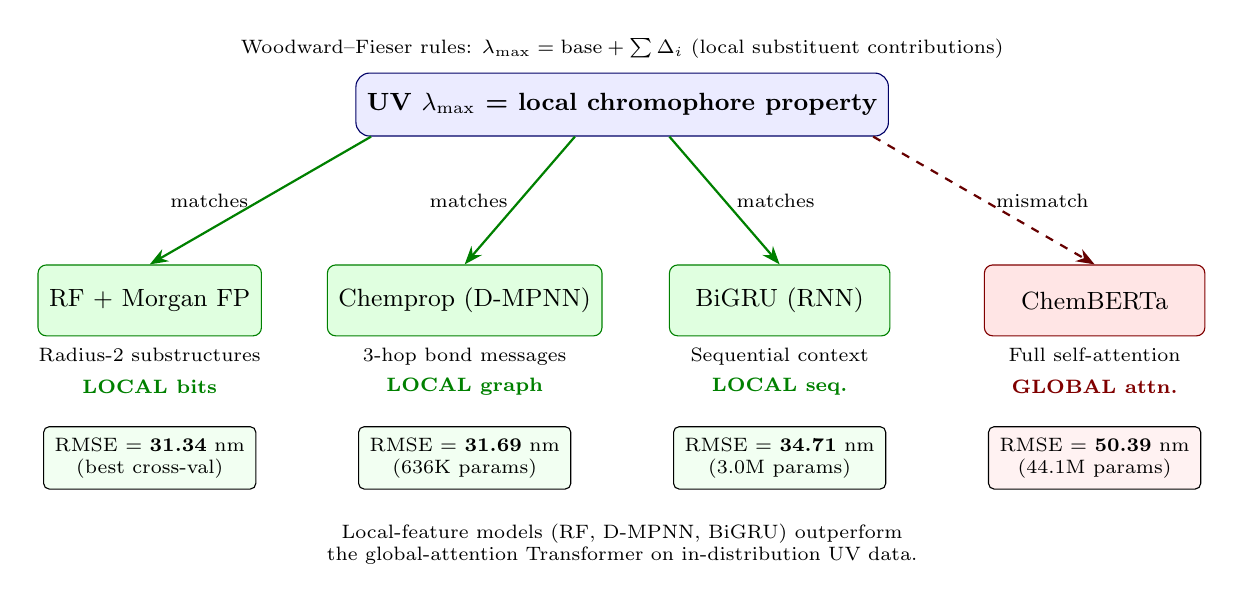
\begin{tikzpicture}[
        >=Stealth,
        box/.style={draw, rounded corners=3pt, minimum width=2.8cm, minimum height=0.9cm, align=center, font=\small},
        localbox/.style={box, fill=green!12, draw=green!50!black},
        globalbox/.style={box, fill=red!10, draw=red!50!black},
        propbox/.style={draw, rounded corners=5pt, fill=blue!8, draw=blue!40!black, minimum width=4cm, minimum height=0.8cm, align=center, font=\small\bfseries},
        annot/.style={font=\scriptsize, text=black},
        every node/.style={inner sep=4pt}
    ]
    % --- Header: UV absorption property ---
    \node[annot] (uvsub) at (0, 5.0) {Woodward--Fieser rules: $\lambda_{\max} = \text{base} + \sum \Delta_i$ (local substituent contributions)};
    \node[propbox, below=1pt of uvsub] (uvprop) {UV $\lambda_{\max}$ = local chromophore property};

    % --- Four model columns ---
    % RF column
    \node[localbox] (rf) at (-6.0, 1.8) {RF + Morgan FP};
    \node[annot, below=0pt of rf] (rfdesc) {Radius-2 substructures};
    \node[font=\scriptsize\bfseries, text=green!50!black] at (-6.0, 0.7) {LOCAL bits};

    % Chemprop column
    \node[localbox] (chemprop) at (-2.0, 1.8) {Chemprop (D-MPNN)};
    \node[annot, below=0pt of chemprop] (chempropdesc) {3-hop bond messages};
    \node[font=\scriptsize\bfseries, text=green!50!black] at (-2.0, 0.7) {LOCAL graph};

    % BiGRU column
    \node[localbox] (bigru) at (2.0, 1.8) {BiGRU (RNN)};
    \node[annot, below=0pt of bigru] (bigrudesc) {Sequential context};
    \node[font=\scriptsize\bfseries, text=green!50!black] at (2.0, 0.7) {LOCAL seq.};

    % ChemBERTa column
    \node[globalbox] (bert) at (6.0, 1.8) {ChemBERTa};
    \node[annot, below=0pt of bert] (bertdesc) {Full self-attention};
    \node[font=\scriptsize\bfseries, text=red!50!black] at (6.0, 0.7) {GLOBAL attn.};

    % --- Arrows from property to models ---
    \draw[->, thick, green!50!black] (uvprop.south west) ++(0.2,0) -- (rf.north) node[midway, left, annot] {matches};
    \draw[->, thick, green!50!black] (uvprop.south) ++(-0.6,0) -- (chemprop.north) node[midway, left, annot] {matches};
    \draw[->, thick, green!50!black] (uvprop.south) ++(0.6,0) -- (bigru.north) node[midway, right, annot] {matches};
    \draw[->, thick, red!40!black, dashed] (uvprop.south east) ++(-0.2,0) -- (bert.north) node[midway, right, annot] {mismatch};

    % --- Result boxes at bottom ---
    \node[draw, rounded corners=2pt, fill=green!5, font=\scriptsize, align=center] (rfres) at (-6.0, -0.2) {RMSE = \textbf{31.34} nm\\(best cross-val)};
    \node[draw, rounded corners=2pt, fill=green!5, font=\scriptsize, align=center] (chempropres) at (-2.0, -0.2) {RMSE = \textbf{31.69} nm\\(636K params)};
    \node[draw, rounded corners=2pt, fill=green!5, font=\scriptsize, align=center] (bigrures) at (2.0, -0.2) {RMSE = \textbf{34.71} nm\\(3.0M params)};
    \node[draw, rounded corners=2pt, fill=red!5, font=\scriptsize, align=center] (bertres) at (6.0, -0.2) {RMSE = \textbf{50.39} nm\\(44.1M params)};

    % --- Bottom citation ---
    \node[annot, text width=12cm, align=center] at (0, -1.3) {Local-feature models (RF, D-MPNN, BiGRU) outperform the global-attention Transformer on in-distribution UV data.};
    \end{tikzpicture}
    \caption{Conceptual alignment between UV absorption physics and model architectures. UV $\lambda_{\max}$ is determined by local chromophore features (conjugation, substituents), favoring models whose inductive bias encodes local molecular neighborhoods. RF (radius-2 fingerprints) and Chemprop (3-hop message passing) achieve nearly identical RMSE, reinforcing the locality hypothesis. The dashed red arrow indicates ChemBERTa's architectural mismatch, though out-of-distribution performance (Table~\ref{tab:wetlab_summary}) reveals complementary strengths from pretraining.}
    \label{fig:local_vs_global}
\end{figure}

Figure~\ref{fig:local_vs_global} illustrates this conceptual alignment: models whose inductive bias matches the locality of the target property (RF encoding radius-2 atom neighborhoods, Chemprop aggregating 3-hop bond messages, BiGRU capturing sequential SMILES context) achieve better in-distribution performance than Transformers whose self-attention distributes information globally~\cite{chenMolecularLanguage2023, jiang2023trangru}.
Notably, Chemprop achieves RMSE = 31.69~nm with only 636K parameters, matching the 31.34~nm of RF despite learning representations from scratch rather than relying on precomputed fingerprints.

ChemBERTa, despite being pretrained on SMILES from the ZINC database and having 44.1M parameters (69$\times$ more than Chemprop), achieves RMSE = 50.39~nm, substantially worse than all local-feature models.
This gap is consistent with the hypothesis that global-attention representations are less sample-efficient for local properties on moderately-sized datasets, though ChemBERTa's superior wetlab generalization suggests pretrained knowledge partially compensates.
ChemBERTa achieves the lowest wetlab MAE on novel compounds (26.3~nm vs.\ 28.6~nm for BiGRU; see Experimental Validation), suggesting that pretrained representations offer complementary generalization advantages despite poor in-distribution performance.

XGBoost trained with MAE loss (pseudo-Huber approximation) performs substantially worse than MSE-trained XGBoost (RMSE 40.75 vs.\ 33.70~nm).
This degradation occurs because MAE loss produces non-smooth gradients at zero error, which interacts poorly with XGBoost's second-order Taylor expansion of the loss function~\cite{chen2016xgboost}; the near-zero Hessian values destabilize leaf weight estimation.
RF does not exhibit this pathology, as tree splitting uses variance reduction rather than gradient optimization.


% --- Solvent Ablation ---
\subsection{Effect of Solvent Information}
\label{sec:solvent_ablation}

To quantify the contribution of solvent information, we compare models trained with and without solvent encoding (Table~\ref{tab:solvent_ablation}).

\begin{table}[htbp]
\centering
\caption{Effect of solvent information on model performance (stratified 5-fold CV). ``+~Solvent'' uses concatenated solute+solvent representations; ``Solute only'' uses solute structure alone.}
\label{tab:solvent_ablation}
\begin{tabular}{lcccc}
\toprule
\textbf{Model} & \textbf{RMSE (nm)} & \textbf{MAE (nm)} & $\boldsymbol{R^2}$ & \textbf{Pearson $r$} \\
\midrule
RF + Solvent          & \textbf{31.34 $\pm$ 1.82} & \textbf{15.16 $\pm$ 0.44} & \textbf{0.914 $\pm$ 0.010} & \textbf{0.956 $\pm$ 0.005} \\
RF Solute only        & 34.13 $\pm$ 1.44          & 16.45 $\pm$ 0.33          & 0.898 $\pm$ 0.008          & 0.948 $\pm$ 0.004 \\
\midrule
Chemprop + Solvent    & 31.69 $\pm$ 3.18          & 16.84 $\pm$ 1.74          & 0.911 $\pm$ 0.016          & 0.955 $\pm$ 0.008 \\
Chemprop Solute only  & 33.78 $\pm$ 2.73          & 16.48 $\pm$ 0.64          & 0.900 $\pm$ 0.015          & 0.949 $\pm$ 0.008 \\
\midrule
BiGRU + Solvent       & 36.45 $\pm$ 1.12          & 20.70 $\pm$ 0.51          & 0.884 $\pm$ 0.006          & 0.940 $\pm$ 0.003 \\
BiGRU Solute only     & 39.03 $\pm$ 1.37          & 22.53 $\pm$ 0.32          & 0.866 $\pm$ 0.009          & 0.931 $\pm$ 0.005 \\
\bottomrule
\end{tabular}
\end{table}

Incorporating solvent information reduces RF RMSE by 8\% (34.13 $\to$ 31.34~nm; paired $t$-test: $t = -11.5$, $p = 0.0003$), Chemprop RMSE by 6\% (33.78 $\to$ 31.69~nm; $t = 4.3$, $p = 0.012$), and BiGRU RMSE by 7\% (39.03 $\to$ 36.45~nm; $t = -3.9$, $p = 0.018$), confirming that the solvent concatenation strategy effectively captures solvatochromic effects across all three model families.
The consistency of the improvement (6--8\% across fingerprint, graph, and recurrent architectures) suggests that solvent information contributes complementary predictive signal regardless of the underlying model architecture or molecular representation.

The improvement from solvent encoding is modest relative to the total prediction error, reflecting the well-established principle that chromophore structure dominates UV absorption~\cite{flemingMolecular2010}, with solvatochromic shifts typically contributing 5--20~nm variation~\cite{reichardt2011solvents}.
Nevertheless, for applications such as ICH~S10~\cite{ICH2013S10} photosafety screening where boundary effects matter, this improvement can be practically significant.


% --- Cross-Dataset Benchmarking ---
\subsection{Cross-Dataset Benchmarking}
\label{sec:cross_dataset}

Table~\ref{tab:cross_dataset} presents results on two external datasets, with published baselines included for direct comparison.

\begin{table}[htbp]
\centering
\caption{Cross-dataset benchmarking using published split protocols. $\dagger$Published results from original papers. Best result among our models in bold for each dataset.}
\label{tab:cross_dataset}
\begin{tabular}{llccc}
\toprule
\textbf{Dataset (Split)} & \textbf{Model} & \textbf{RMSE (nm)} & \textbf{MAE (nm)} & $\boldsymbol{R^2}$ \\
\midrule
\multirow{5}{*}{Deep4Chem (80/10/10)}
  & GCNN$^\dagger$            & 26.6   & ---    & ---   \\
  & Our Chemprop              & \textbf{19.13}  & \textbf{10.66}  & \textbf{0.967} \\
  & Our RF                    & 22.70  & 11.32  & 0.954 \\
  & Our ChemBERTa             & 35.90  & 17.43  & 0.884 \\
  & Our BiGRU                 & 27.07  & 17.22  & 0.934 \\
\midrule
\multirow{7}{*}{Jung 2024 (72/18/10)}
  & Multifidelity$^\dagger$   & 31.3   & 14.6   & 0.91  \\
  & GBFS$^\dagger$            & 32.2   & 16.2   & 0.91  \\
  & DR-CNN$^\dagger$          & 44.4   & 23.3   & 0.82  \\
  & Our Chemprop              & \textbf{27.36}  & \textbf{15.50}  & \textbf{0.936} \\
  & Our RF                    & 29.82  & 15.31  & 0.924 \\
  & Our ChemBERTa             & 38.27  & 19.27  & 0.874 \\
  & Our BiGRU                 & 36.31  & 21.54  & 0.887 \\
\bottomrule
\end{tabular}
\end{table}

\textbf{Deep4Chem.}
Our Chemprop D-MPNN achieves RMSE = 19.13~nm, surpassing both our RF (22.70~nm) and the published GCNN baseline of 26.6~nm~\cite{joung2021deep} by 28\%.
RF also outperforms the GCNN by 15\%, and BiGRU performs competitively (RMSE = 27.07~nm), while ChemBERTa (35.90~nm) trails behind.
That a 2D GNN trained from scratch outperforms all other models on this dataset suggests that learned graph representations can capture structural patterns beyond what fixed fingerprints encode, particularly when the training set is large enough to learn effective bond-level features.

\textbf{Jung et al.\ (2024).}
Chemprop again achieves the best result (RMSE = 27.36~nm), followed closely by RF (29.82~nm), both outperforming the published multifidelity (31.3~nm) and GBFS (32.2~nm) approaches.
BiGRU (RMSE = 36.31~nm) and ChemBERTa (38.27~nm) fall between the GBFS and DR-CNN published baselines.
Our top two models use simpler architectures than the published methods (which involve feature selection pipelines and multi-task learning, respectively), yet achieve superior performance.

Across both external datasets, Chemprop achieves the best performance, followed by RF, with both consistently outperforming BiGRU and ChemBERTa, reinforcing the finding that local-feature models (graph message passing and fingerprints) excel at in-distribution prediction. We note (as discussed in Section~\ref{sec:dataset}) that the Deep4Chem results should be read as in-distribution validation rather than an OOD test, because Deep4Chem shares 77\% of its solutes with our primary training data; the Jung 2024 results, with $\sim$50\% solute overlap and a separate experimental provenance, constitute the more rigorous external benchmark.

% --- Performance on Non-Local Subsets ---
\subsection{Performance on Non-Local Subsets}
\label{sec:nonlocal_subsets}

The benchmarks above pool molecules whose absorption is plausibly governed by local substitution patterns with molecules where the chromophore spans the entire $\pi$-system---donor--acceptor charge-transfer dyes, low-gap polymethines, BODIPYs, and other classes where global electronic effects and longer conjugation paths are expected to dominate. To examine whether the locality argument introduced in Section~\ref{sec:model_comparison} continues to hold for this second class, we partitioned the Joung+Beard test folds into subsets enriched for non-local effects and recomputed per-model error metrics within each subset.

Subset definitions: \textit{long-wavelength} compounds ($\lambda_{\max} > 500$~nm or $> 600$~nm); \textit{donor--acceptor} (D-A) molecules containing at least one $\pi$-donor substituent (aryl-NH$_2$, aryl-NHR, aryl-NR$_2$, aryl-OH, aryl-OR, aryl-SH, aryl-SR) \emph{and} at least one $\pi$-acceptor (NO$_2$, CN, CHO, ketone, COOH/COOR/amide, SO$_2$R, CF$_3$, pyridinium, dicyanovinyl) attached to a conjugated $sp^2$ centre; D-A-D molecules with $\geq 2$ donor matches and $\geq 1$ acceptor; \textit{azo} dyes (Ar--N$=$N--Ar); and BODIPY cores (BF$_2$ bridging two ring nitrogens). The exact SMARTS patterns and per-rule molecule counts are listed in Supporting Information Section~S7. The union of all non-local categories covers 49\% of the dataset, with the individual subset sizes ranging from 264 (azo) to 6{,}059 (D-A) molecules.

\begin{table}[htbp]
\centering
\caption{RMSE (nm, mean $\pm$ std across the five stratified test folds) restricted to non-local subsets of the Joung+Beard dataset. $n$ is the per-fold subset size averaged across folds. Best result on each row in bold; ties within $0.2$~nm are both bolded. MAE and $R^2$ on the same subsets are reported in Supporting Information Table~S14.}
\label{tab:nonlocal_subsets}
\small
\begin{tabular}{lcccccc}
\toprule
\textbf{Subset} & $n$ & \textbf{RF} & \textbf{Chemprop} & \textbf{BiGRU} & \textbf{ChemBERTa} & \textbf{XGBoost} \\
\midrule
Full dataset                     & 3751 & \textbf{31.3 $\pm$ 2.0} & 31.7 $\pm$ 3.6  & 34.7 $\pm$ 1.6  & 50.4 $\pm$ 2.6   & 33.7 $\pm$ 1.8 \\
$\lambda_{\max} > 500$~nm        &  777 & 52.0 $\pm$ 5.3          & \textbf{45.3 $\pm$ 7.7}  & 52.5 $\pm$ 5.9  & 98.4 $\pm$ 6.1   & 51.3 $\pm$ 5.3 \\
$\lambda_{\max} > 600$~nm        &  315 & 69.5 $\pm$ 9.3          & \textbf{60.9 $\pm$ 15.2} & 69.6 $\pm$ 10.8 & 148.2 $\pm$ 10.0 & 67.8 $\pm$ 9.3 \\
Azo (Ar--N$=$N--Ar)              &   53 & 32.6 $\pm$ 7.6          & \textbf{29.2 $\pm$ 4.3}  & 38.9 $\pm$ 6.3  & 37.3 $\pm$ 4.3   & 34.3 $\pm$ 6.1 \\
D-A                              & 1212 & 24.3 $\pm$ 0.7          & \textbf{23.1 $\pm$ 2.7}  & 28.1 $\pm$ 1.0  & 43.7 $\pm$ 1.6   & 27.0 $\pm$ 0.9 \\
D-A-D                            &  438 & 26.4 $\pm$ 2.7          & \textbf{24.0 $\pm$ 1.5}  & 30.9 $\pm$ 2.6  & 39.5 $\pm$ 1.3   & 28.6 $\pm$ 2.8 \\
BODIPY core                      &  353 & \textbf{22.3 $\pm$ 4.3} & \textbf{22.4 $\pm$ 1.9}  & 27.2 $\pm$ 5.5  & 69.7 $\pm$ 8.3   & 24.7 $\pm$ 2.9 \\
\bottomrule
\end{tabular}
\end{table}

Two trends are visible. First, every model degrades sharply on long-wavelength compounds: RMSE roughly doubles when restricting to $\lambda_{\max} > 500$~nm and more than doubles for $\lambda_{\max} > 600$~nm. The effect is seen across all five architectures, but ChemBERTa exhibits an extreme version of it (RMSE = 98 and 148~nm respectively, with negative $R^2$ on both subsets): its predictions collapse to an essentially constant value around 600~nm, the prediction-ceiling artefact visible in Figure~\ref{fig:parity_5models} and diagnosed in detail in Section~\ref{sec:error_analysis}. For the other four models the degradation is consistent with two compounding factors identified in prior work on these datasets~\cite{beard2019comparative,joung2021deep}: data scarcity in the deep-coloured region of $\lambda$-space, and the greater structural complexity of low-gap chromophores (extended polyenes, push--pull cyanines, BODIPYs, phthalocyanines), many of which carry charge-transfer character whose accurate description requires global rather than local features.

Second, the rank between RF and Chemprop is \emph{not stable} across subsets. On the full dataset the two are statistically indistinguishable ($p = 0.77$; Section~\ref{sec:model_comparison}), but on every subset enriched for non-local effects Chemprop edges out RF: by $1.2$~nm on D-A compounds, $2.4$~nm on D-A-D, $3.4$~nm on azo dyes, and $6.7$~nm on $\lambda_{\max} > 500$~nm. BiGRU and ChemBERTa do not show this pattern. The Chemprop advantage on the non-local subsets is small in absolute terms and remains within one fold-standard-deviation for the smaller subsets, so this result should be read as suggestive rather than conclusive: it is consistent with the locality argument---message-passing GNNs benefit relatively more when the property is governed by global rather than local features---without overturning the headline observation that RF and Chemprop are within noise of each other on the dataset as a whole. The one row where RF holds its ground is on BODIPYs (RMSE = 22.3 vs.\ 22.4~nm for Chemprop, an effective tie), a class whose rigid, conserved scaffold means that absorption is largely explained by short-range substitution patterns the fingerprint already captures.


% --- Error Analysis ---
\subsection{Error Analysis}
\label{sec:error_analysis}

\begin{figure}[htbp]
    \centering
    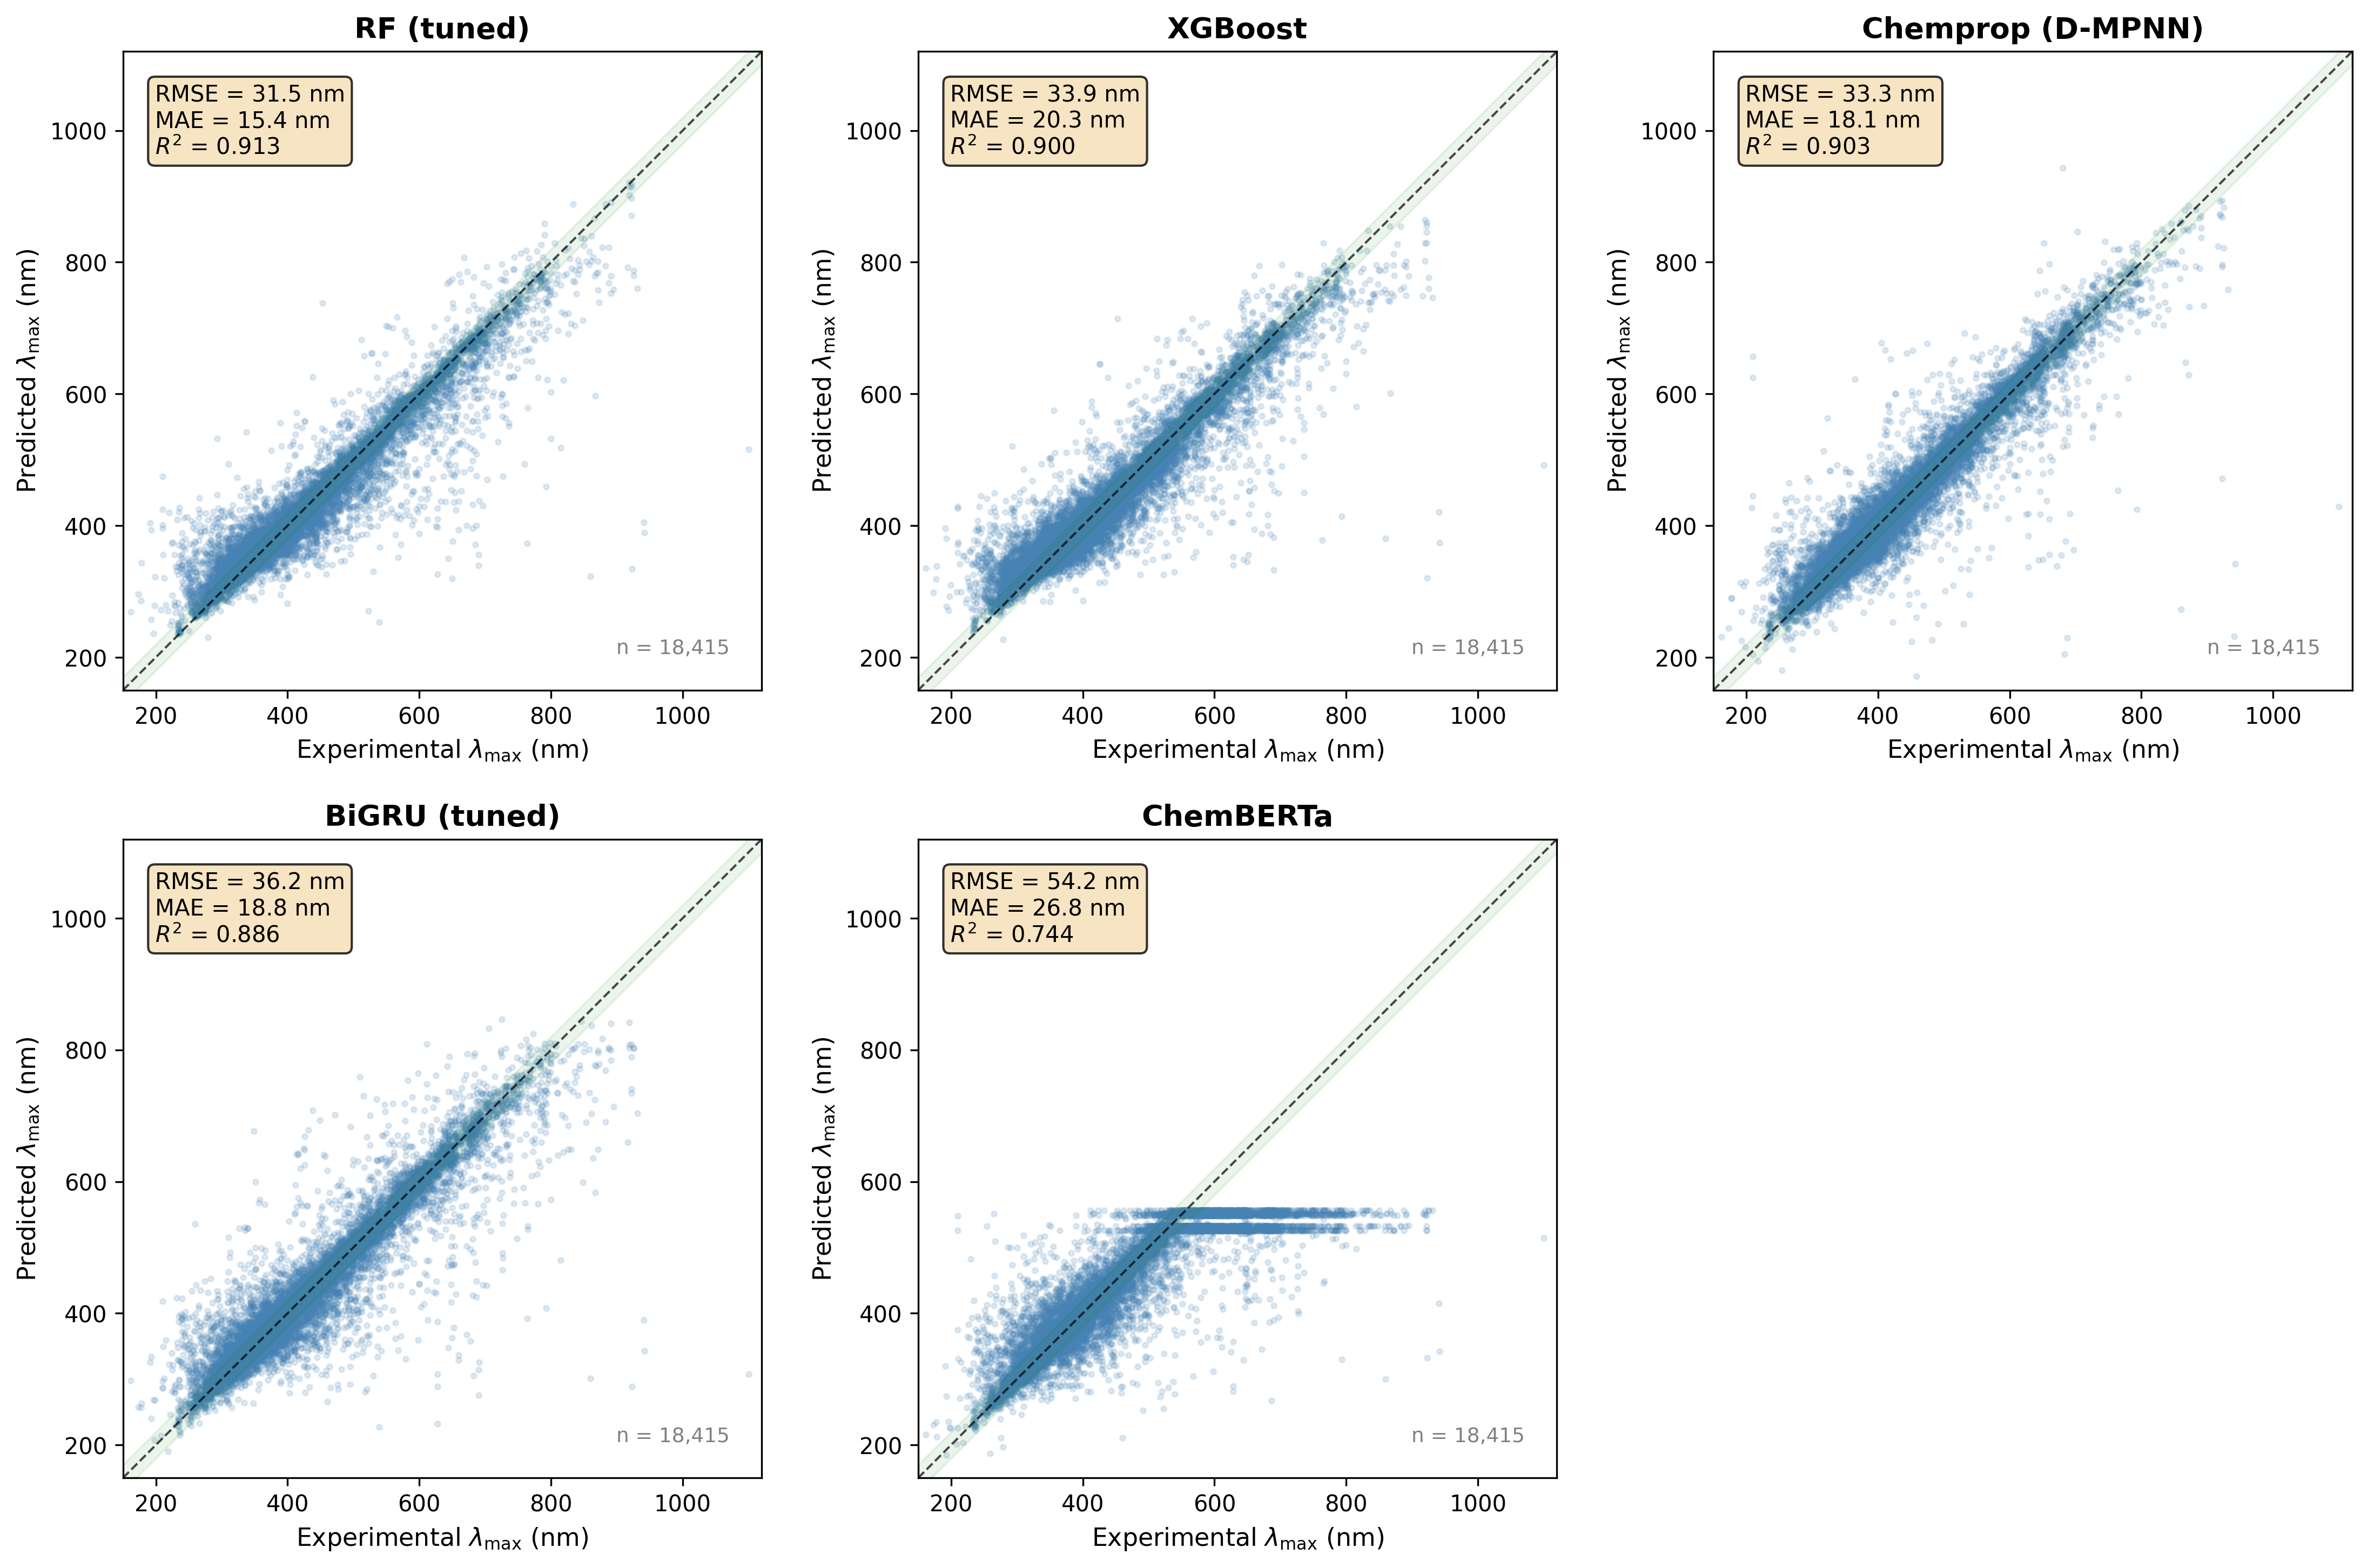
\includegraphics[width=0.95\textwidth]{results/parity_plot_5models.png}
    \caption{Parity plots for all five model families (pooled 5-fold CV predictions). Green shaded bands indicate $\pm 20$~nm from perfect prediction. RF and Chemprop show the tightest clustering around the diagonal, while ChemBERTa exhibits the most scatter, particularly for long-wavelength compounds. All models show increased error for $\lambda_{\max} > 500$~nm.}
    \label{fig:parity_5models}
\end{figure}

\begin{figure}[htbp]
    \centering
    \begin{subfigure}[t]{0.48\textwidth}
        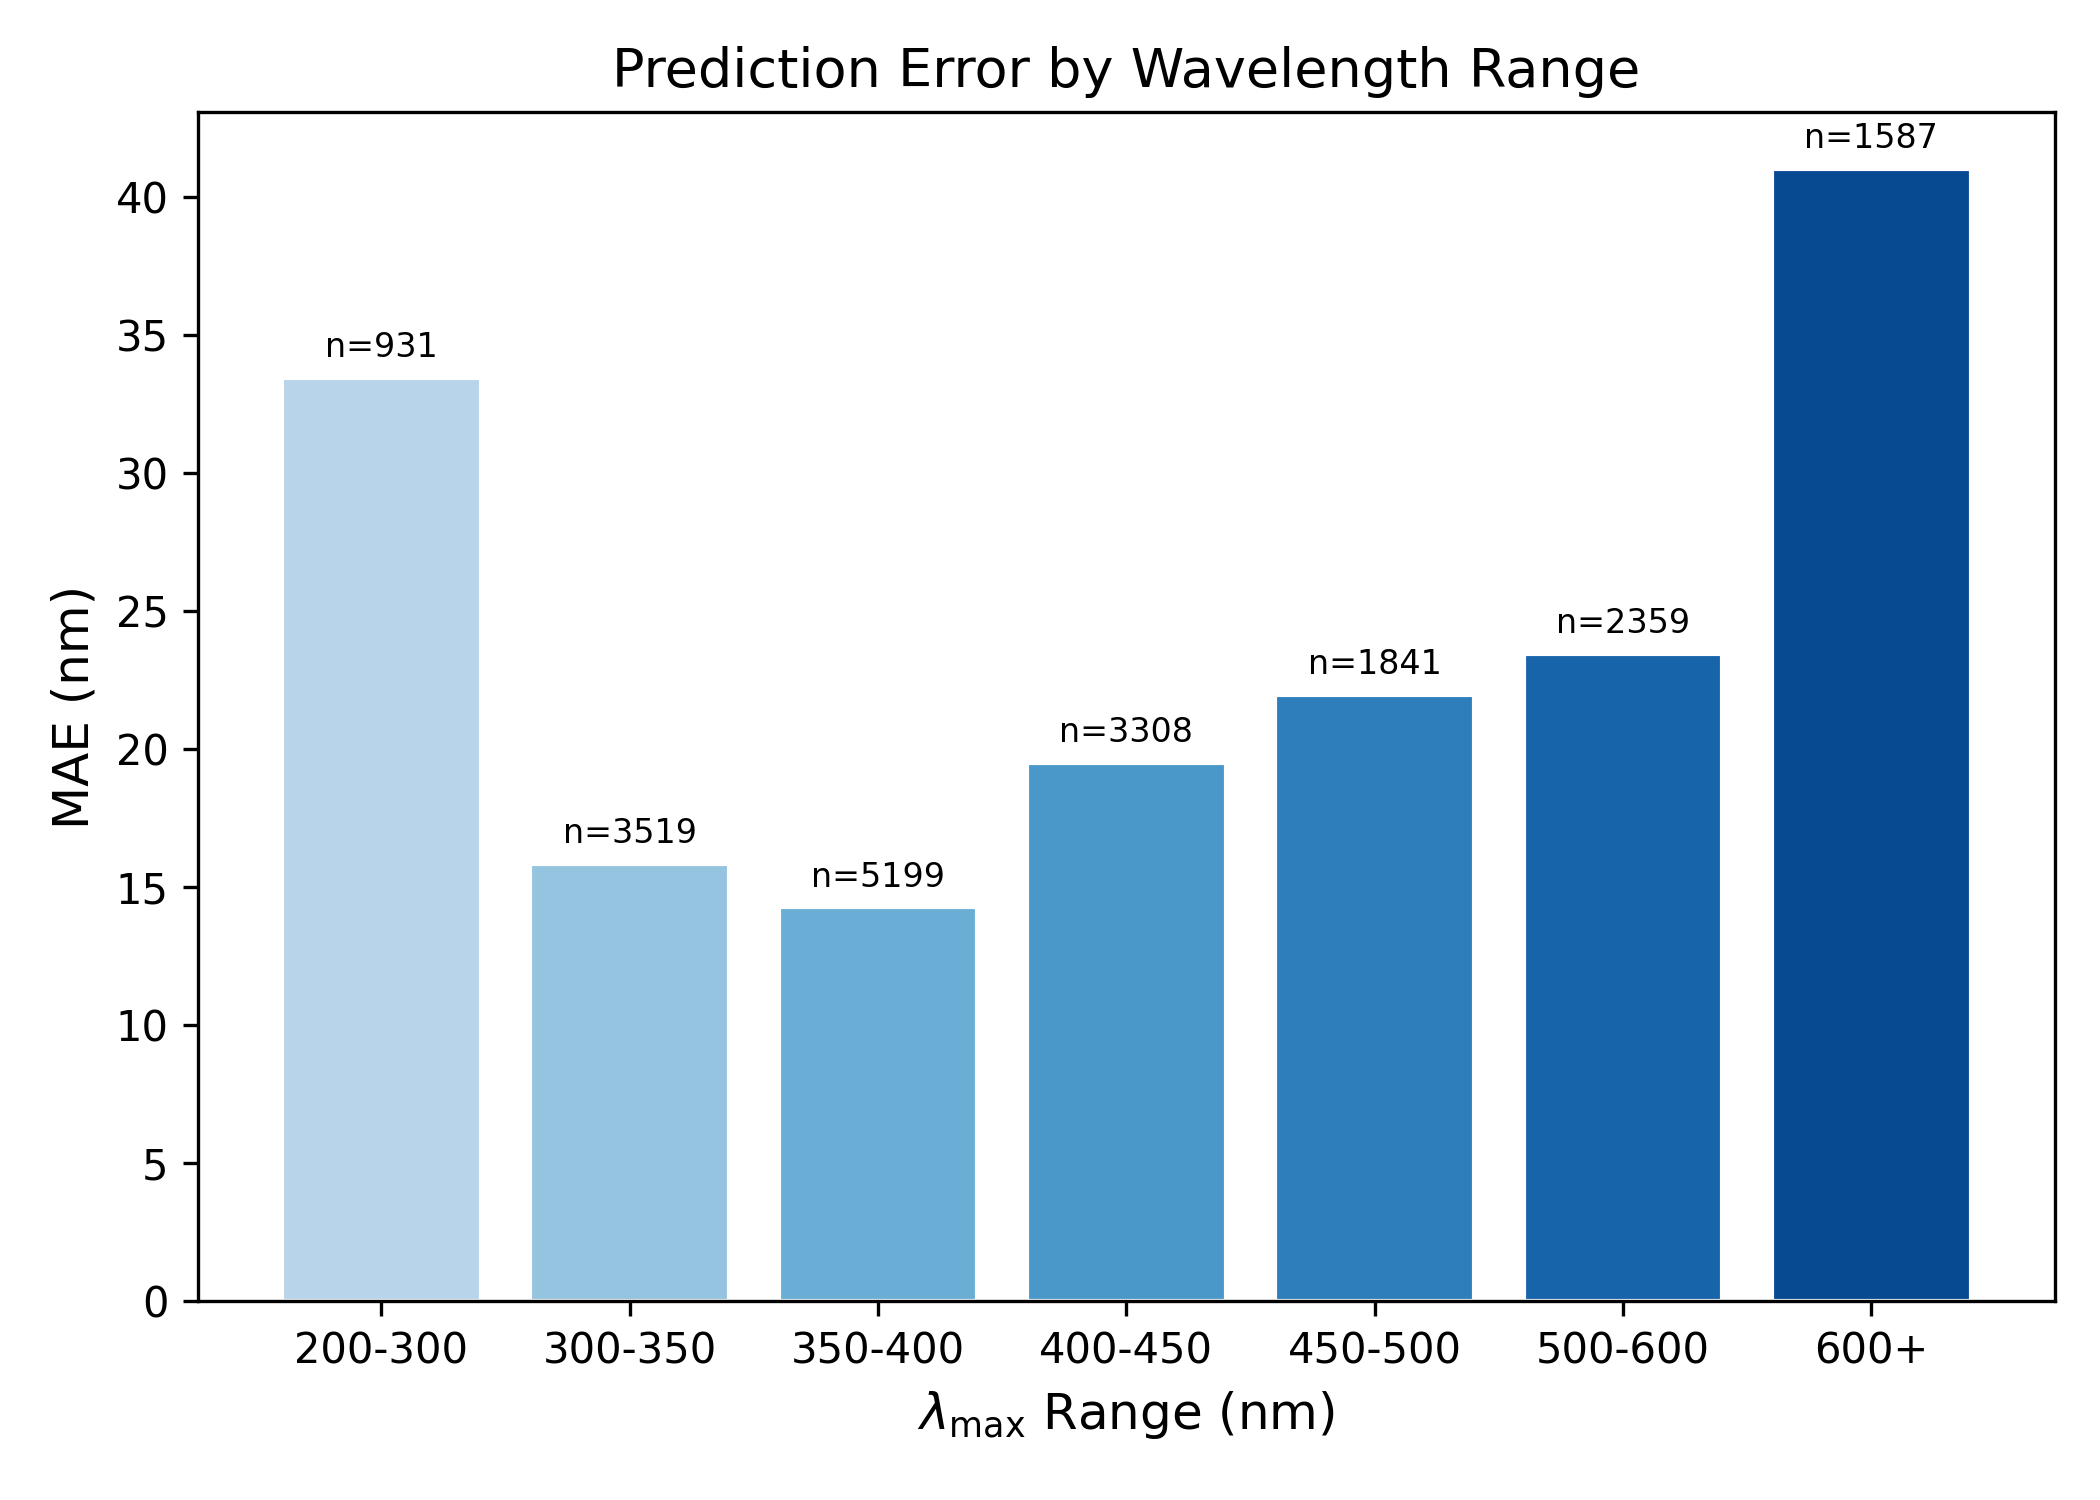
\includegraphics[width=\textwidth]{results/error_by_wavelength.png}
        \caption{MAE by wavelength range. Prediction accuracy is highest for $\lambda_{\max} < 400$~nm where training data is most abundant.}
    \end{subfigure}
    \hfill
    \begin{subfigure}[t]{0.48\textwidth}
        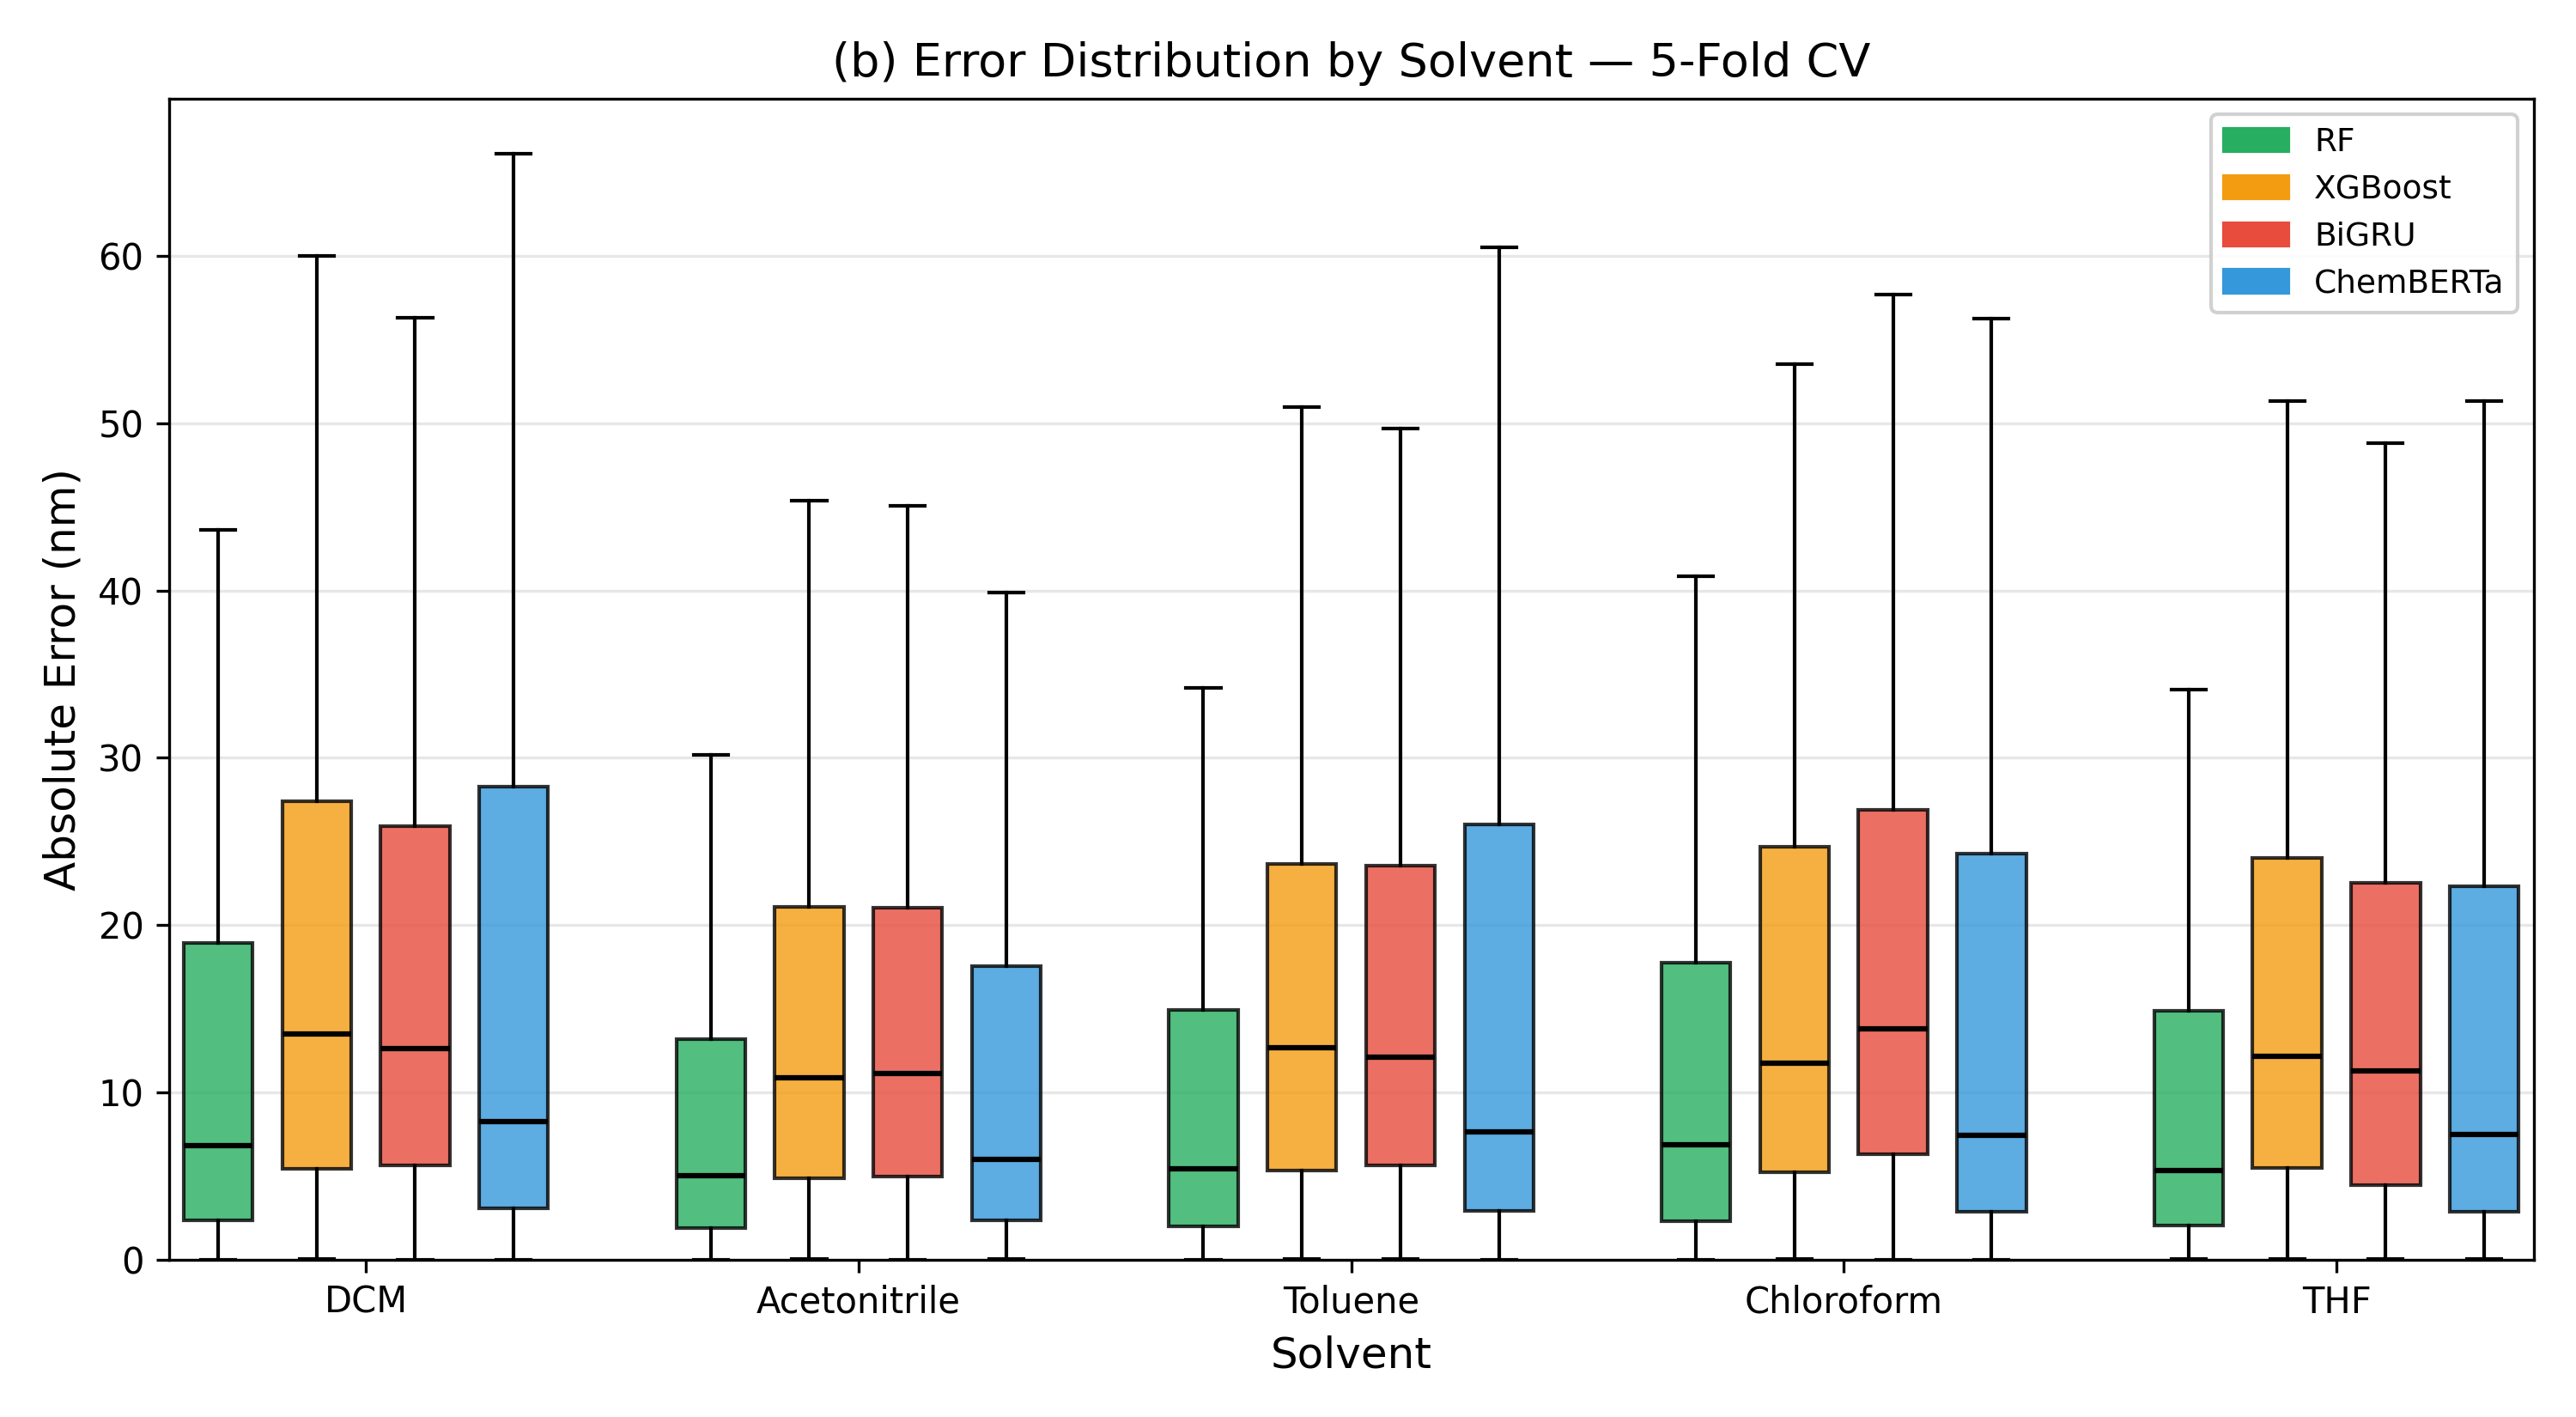
\includegraphics[width=\textwidth]{results/error_by_solvent.png}
        \caption{MAE by solvent type for the five most common solvents in the dataset.}
    \end{subfigure}
    \caption{Error breakdown by wavelength range and solvent type for all five model families (pooled 5-fold CV predictions).}
    \label{fig:error_breakdown}
\end{figure}

Figure~\ref{fig:parity_5models} shows parity plots for all five model families on the primary dataset.
RF predictions cluster most tightly around the diagonal, consistent with its lowest RMSE, while ChemBERTa shows the broadest scatter.
All models perform best in the 250--400~nm range where training data is most abundant (Figure~\ref{fig:error_breakdown}a).
Errors increase substantially for $\lambda_{\max} > 500$~nm, reflecting both data scarcity in this wavelength range and the greater structural complexity of long-wavelength chromophores, many of which are extended conjugated systems (porphyrins, phthalocyanines, cyanine dyes) with properties strongly dependent on 3D geometry~\cite{flemingMolecular2010}.
Error distributions across the five most common solvents (Figure~\ref{fig:error_breakdown}b) show relatively consistent performance, with slightly higher errors for chloroform and dichloromethane.


% --- Model Interpretability and Practical Considerations ---
\subsection{Model Interpretability and Practical Considerations}
\label{sec:interpretability}

A key advantage of fingerprint-based models is their interpretability through feature importance analysis.
In contrast to deep learning models, which are traditionally viewed as less interpretable, Random Forest models provide direct access to the contribution of each input feature through Gini importance, a measure of how much each feature reduces prediction variance across all decision trees in the ensemble.

Since each bit in a Morgan fingerprint corresponds to a specific molecular substructure (a circular neighborhood of radius $\leq 2$ around each atom), high-importance bits can be decoded back to chemically meaningful structural motifs.
We averaged Gini importances across all five fold models and decoded the top features using RDKit.

\begin{figure*}[htbp]
    \centering
    \begin{subfigure}[t]{0.48\textwidth}
        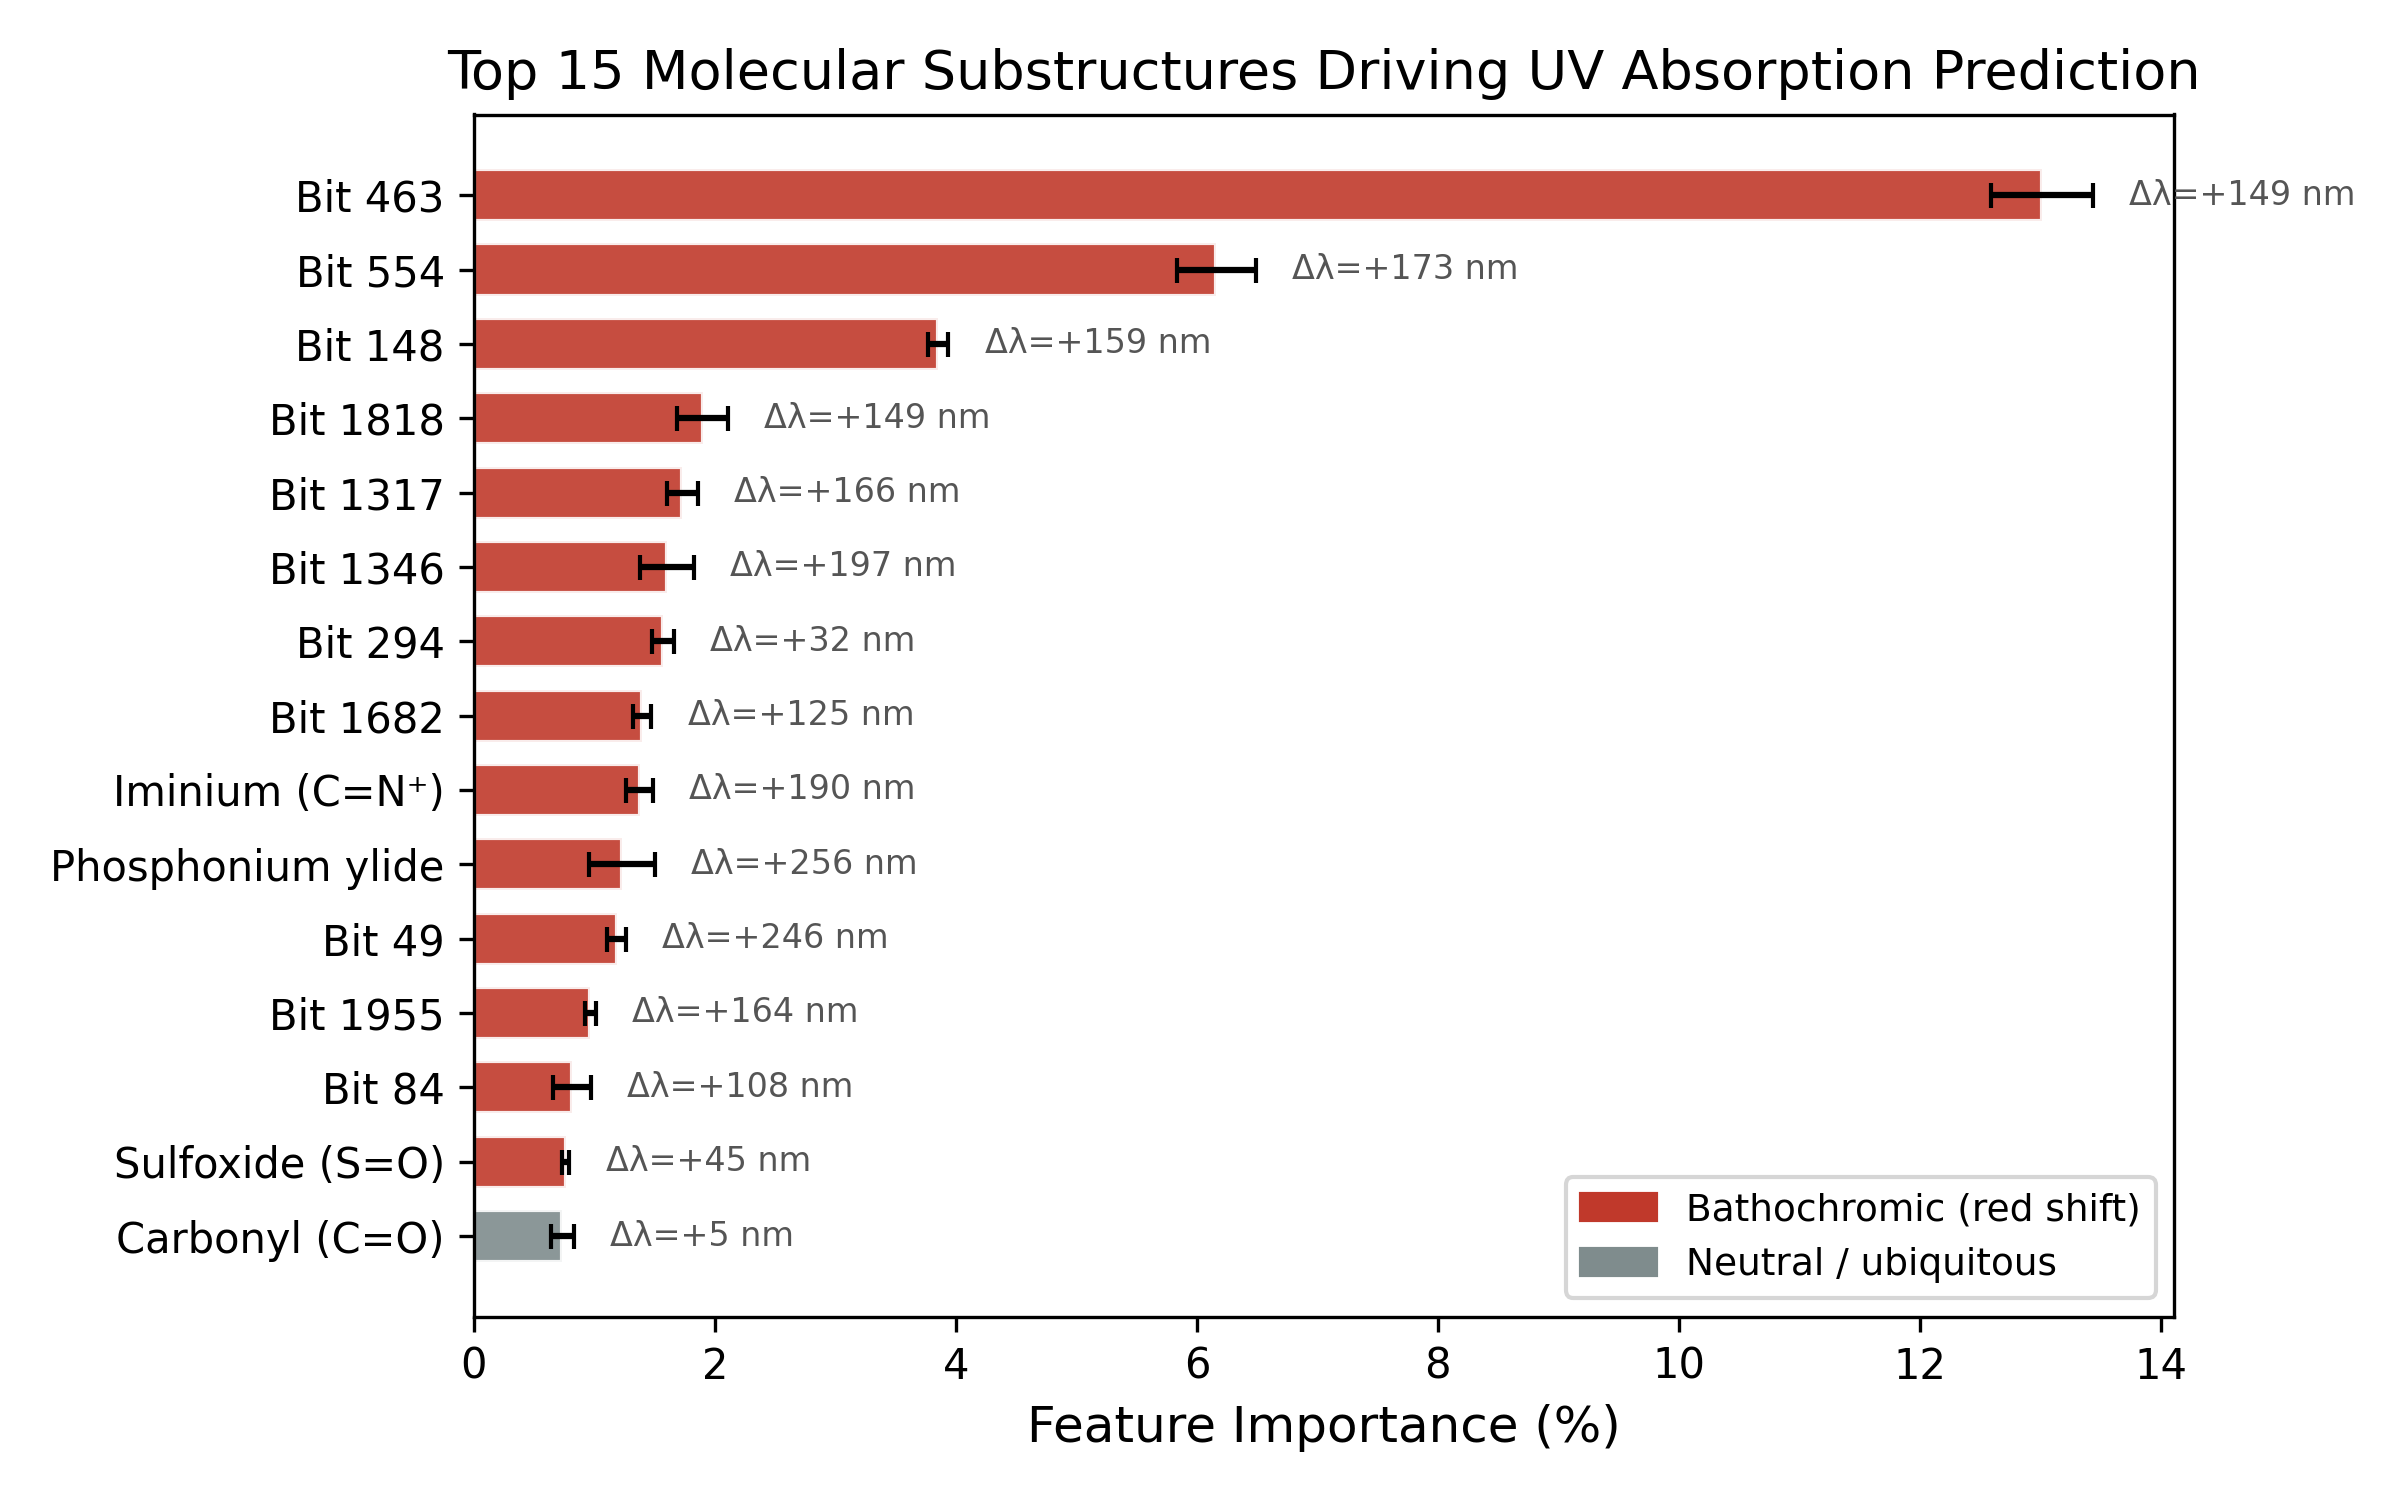
\includegraphics[width=\textwidth]{results/rf_feature_importance.png}
        \caption{Top 15 Morgan fingerprint bits ranked by Gini importance, with mean $\Delta\lambda_{\max}$ annotations. Red indicates bathochromic (red-shifting) substructures; gray indicates neutral or ubiquitous features. All high-importance features are bathochromic, reflecting the dominance of conjugation-extending motifs in determining $\lambda_{\max}$.}
    \end{subfigure}
    \hfill
    \begin{subfigure}[t]{0.48\textwidth}
        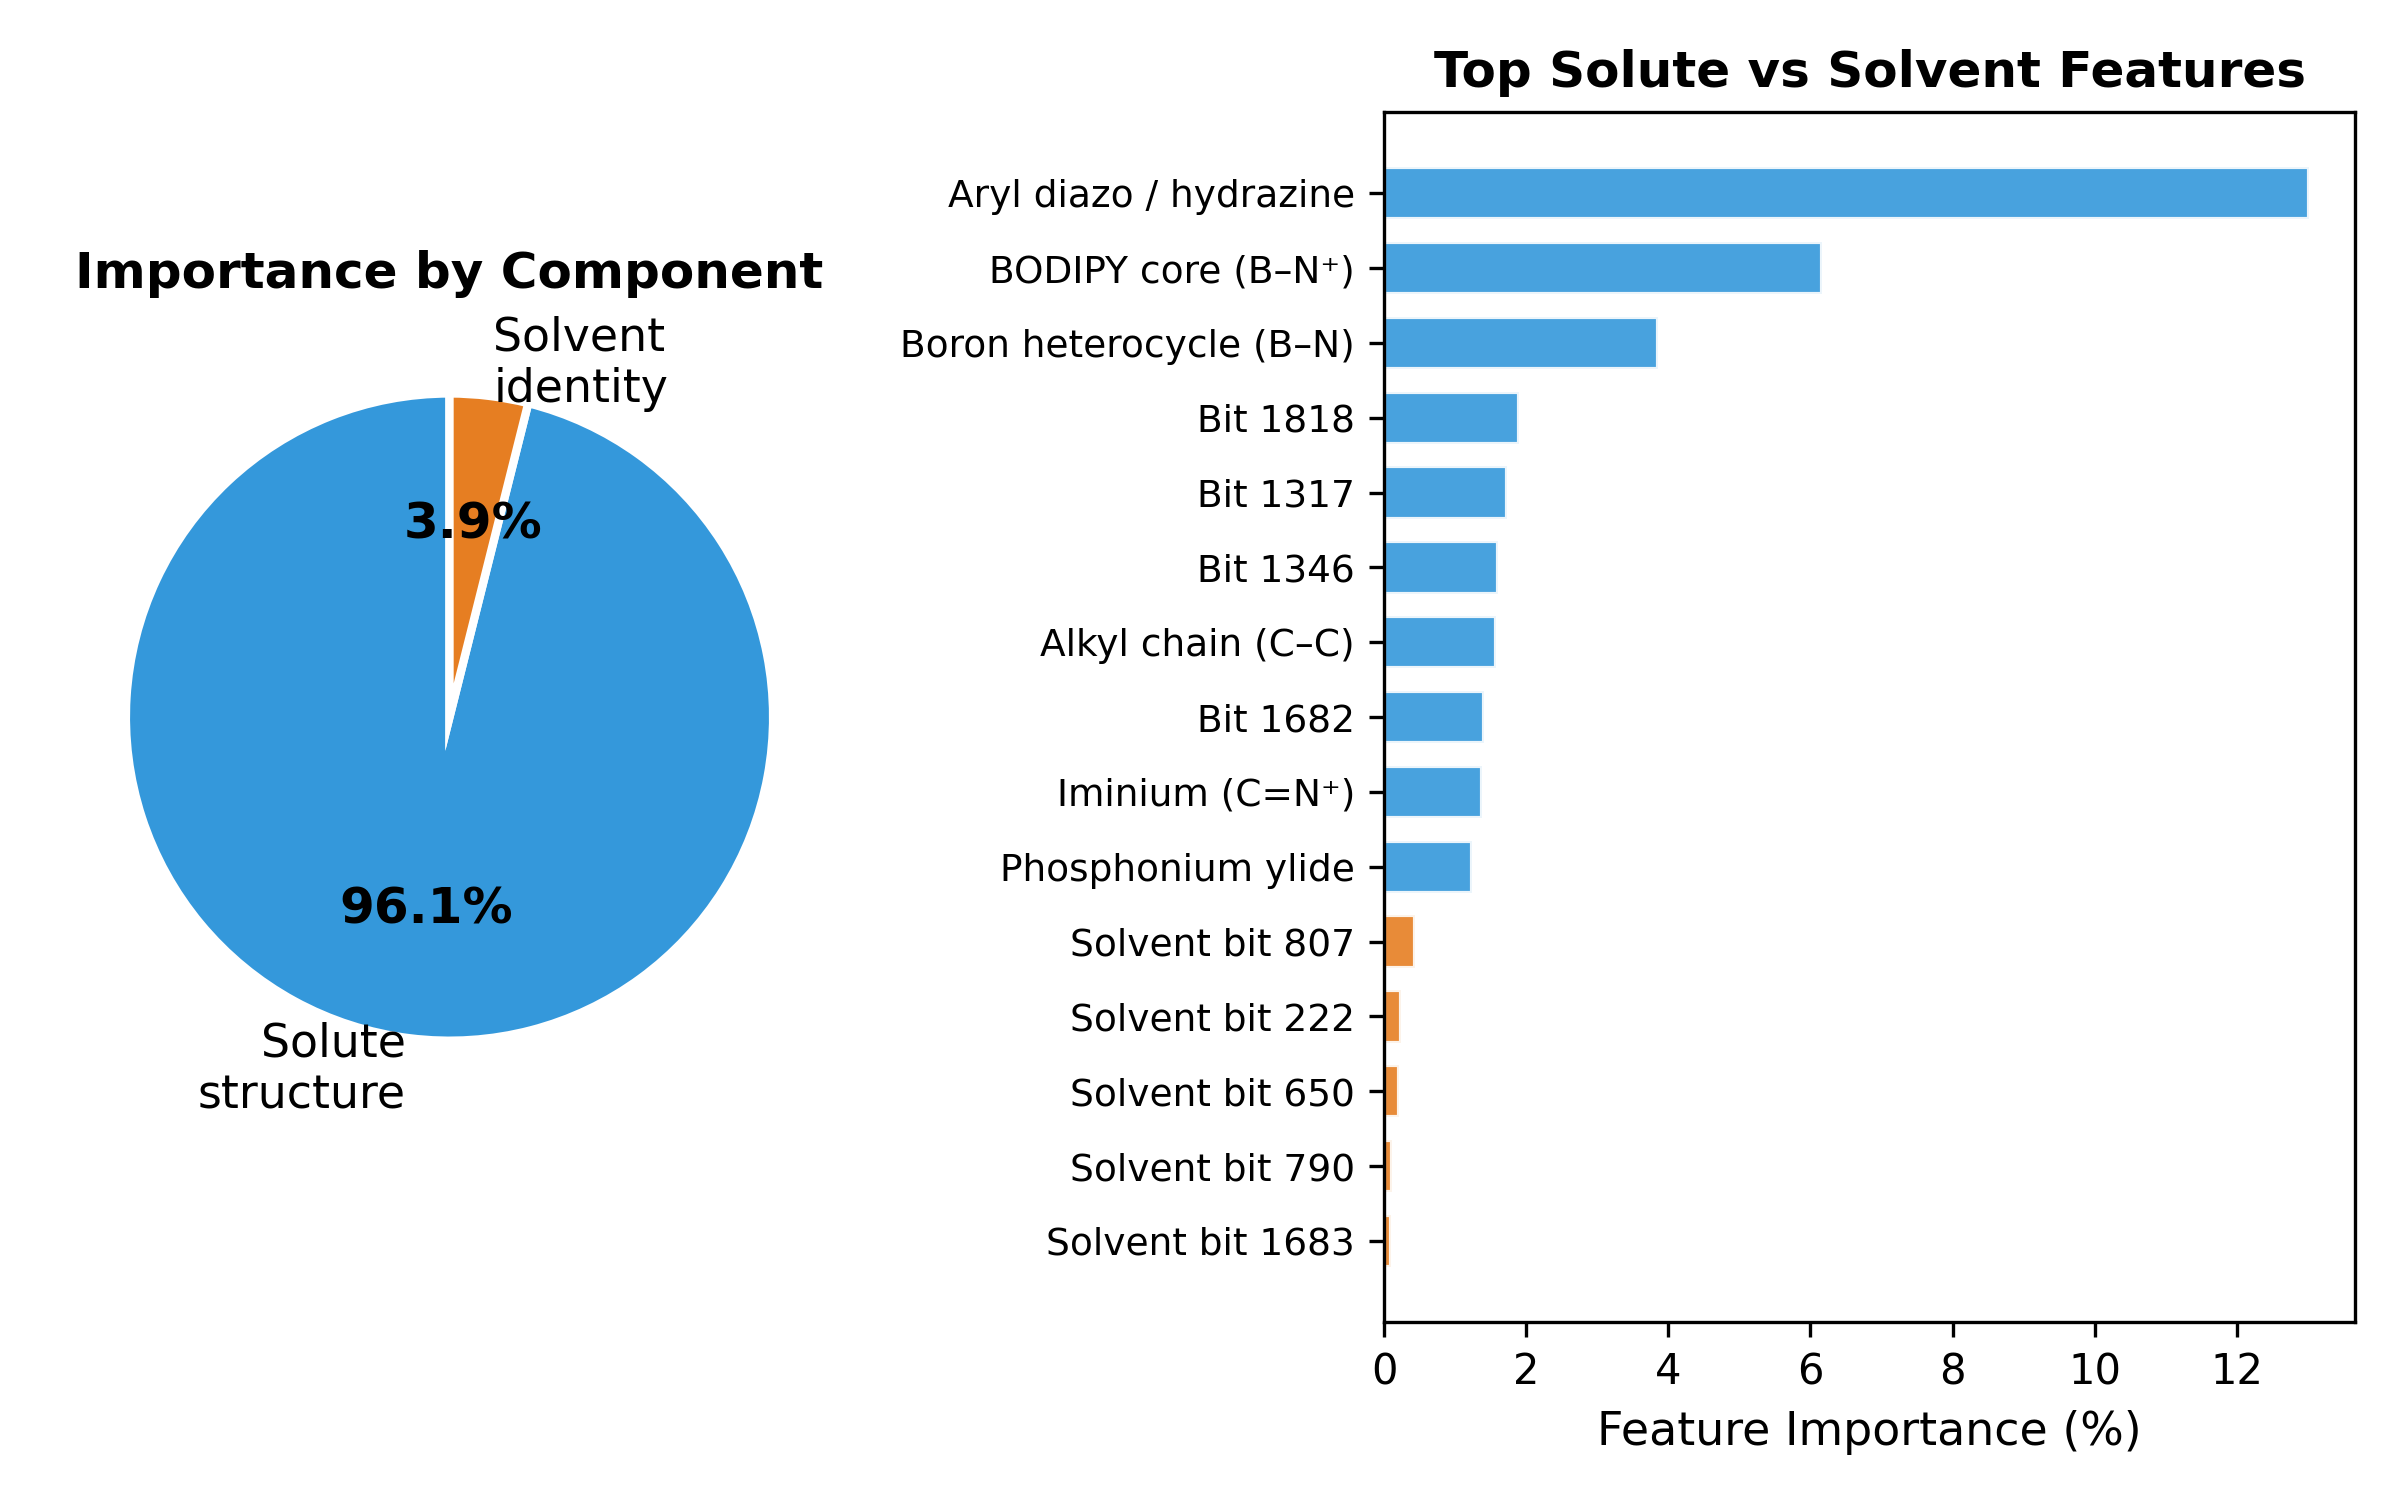
\includegraphics[width=\textwidth]{results/rf_solute_vs_solvent.png}
        \caption{Relative importance of solute vs.\ solvent fingerprint bits. Solute structure accounts for 96.1\% of total feature importance.}
    \end{subfigure}
    \caption{RF feature importance analysis. The model learns chemically meaningful patterns: the top features correspond to known chromophore motifs that produce large bathochromic shifts.}
    \label{fig:rf_interpretability}
\end{figure*}

\begin{figure}[htbp]
    \centering
    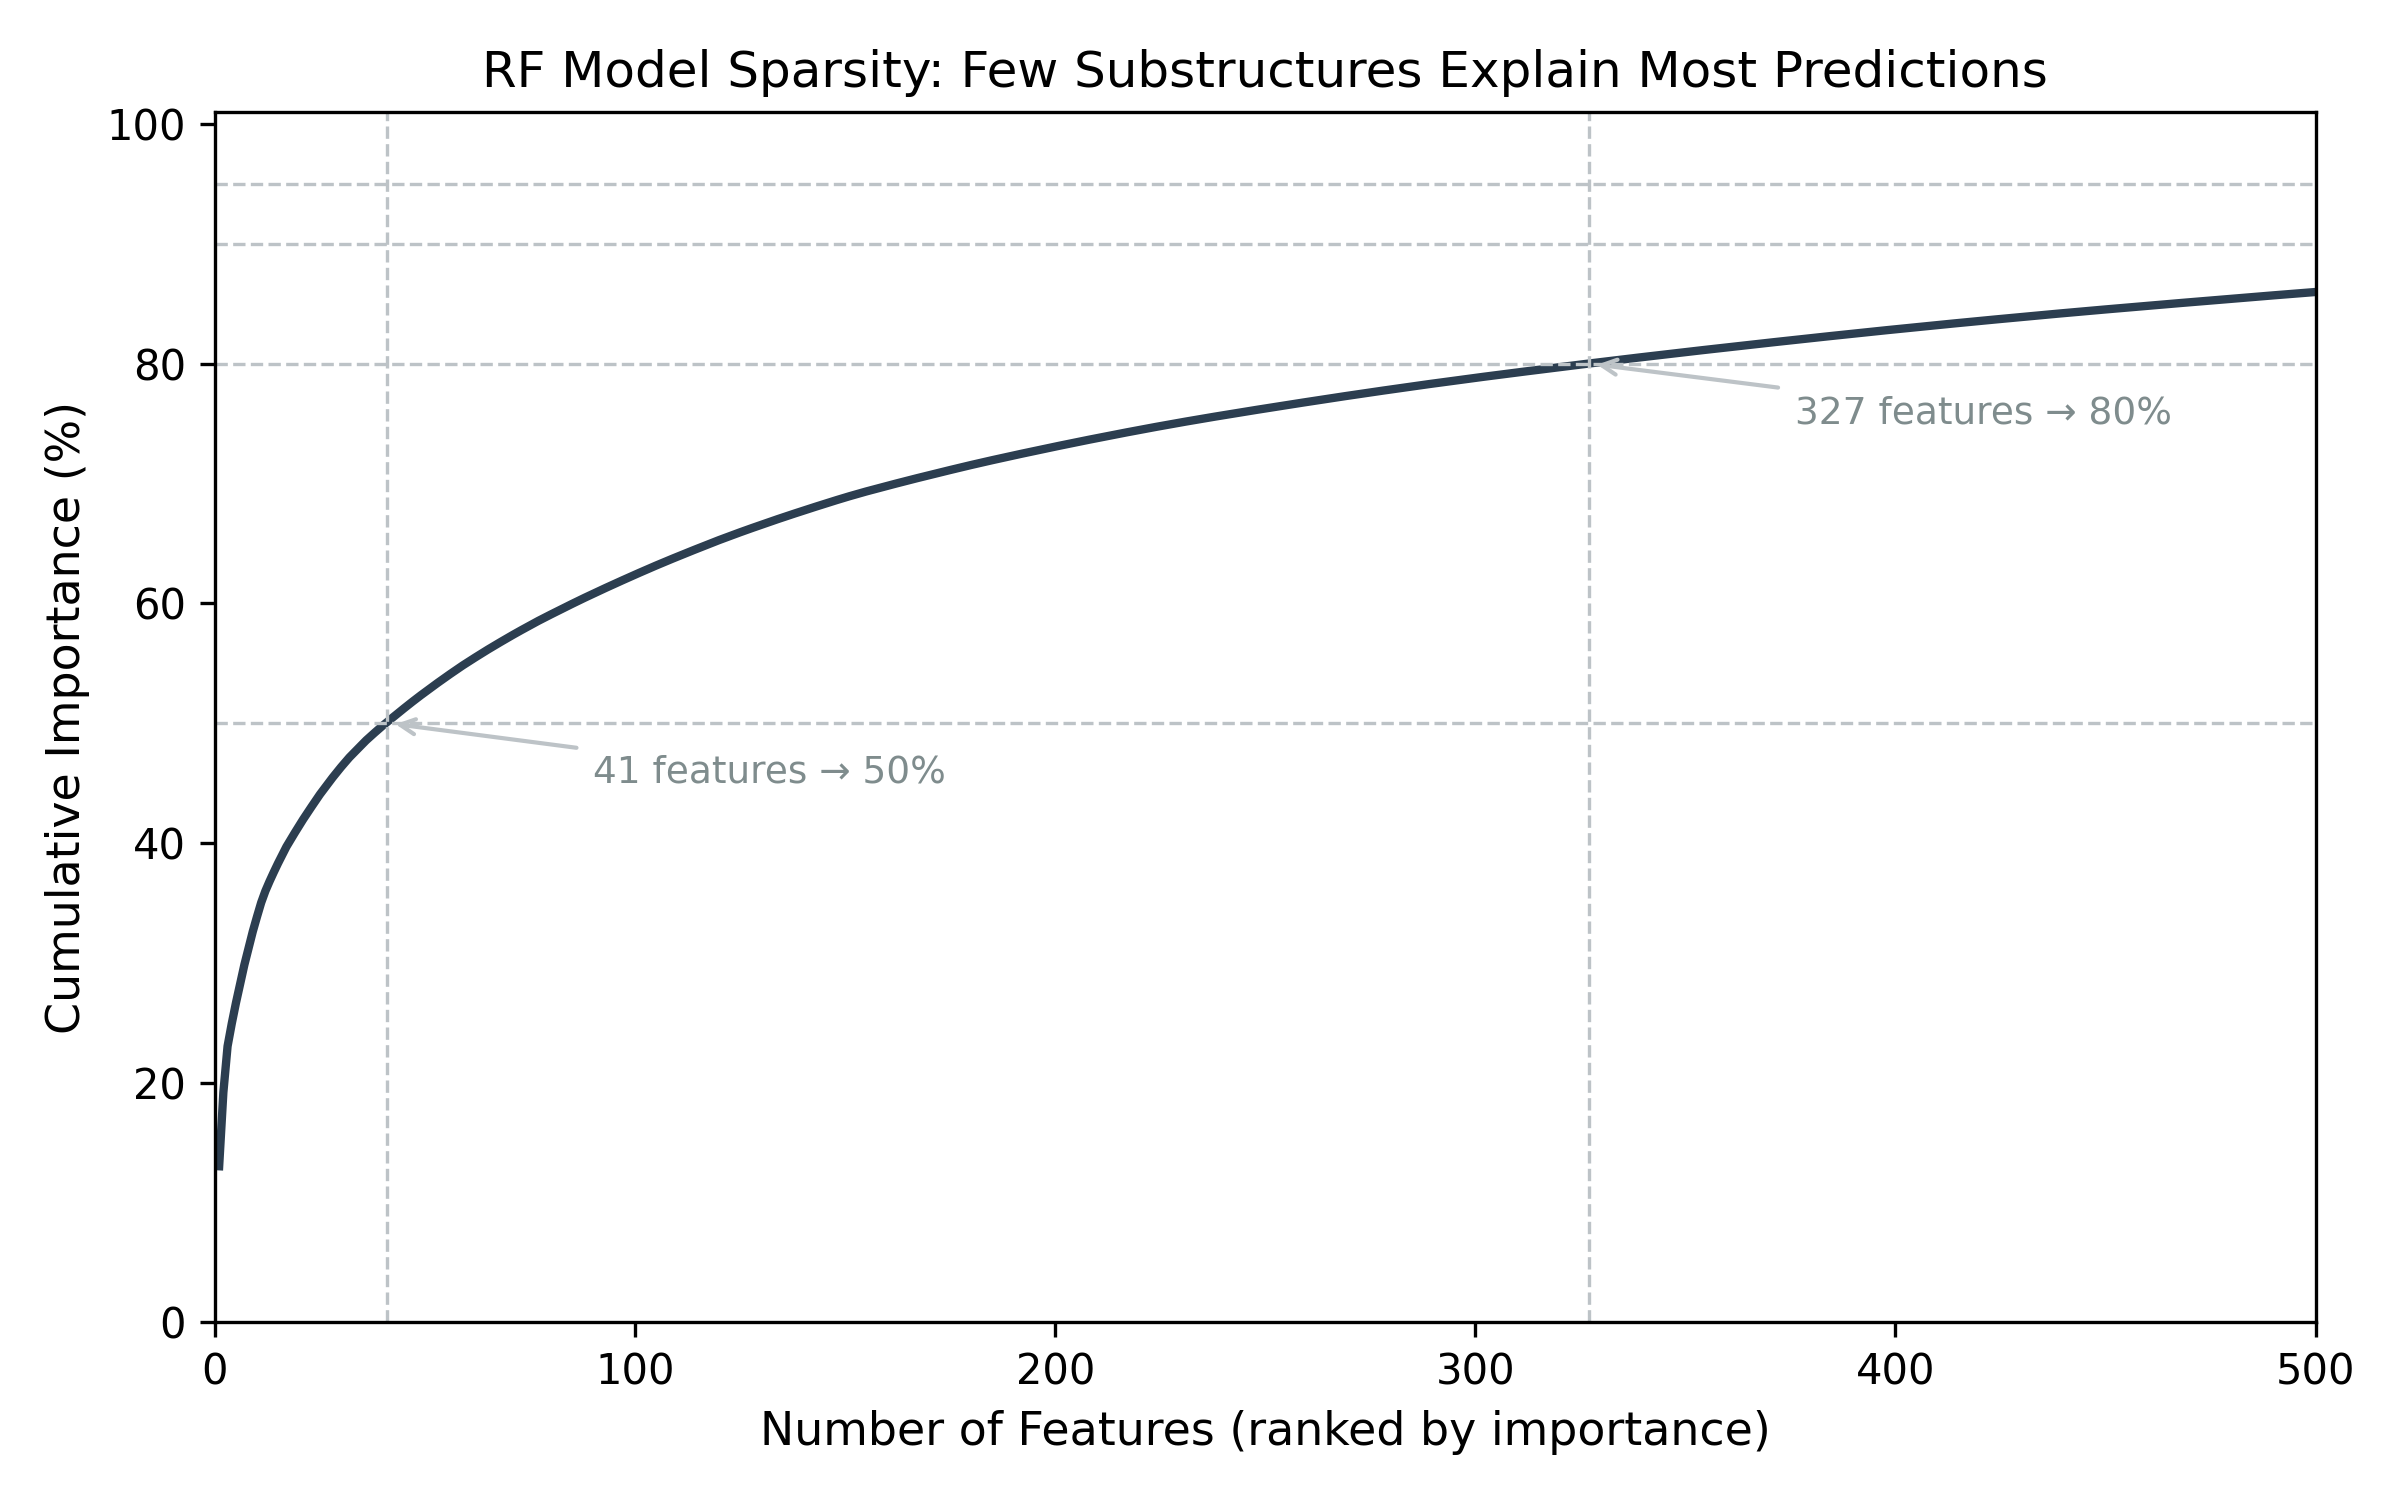
\includegraphics[width=0.65\textwidth]{results/rf_cumulative_importance.png}
    \caption{Cumulative feature importance. The top 41 features (out of 4096) account for 50\% of total importance, and 327 features reach 80\%, indicating a sparse, interpretable model.}
    \label{fig:rf_cumulative}
\end{figure}

\begin{figure}[htbp]
    \centering
    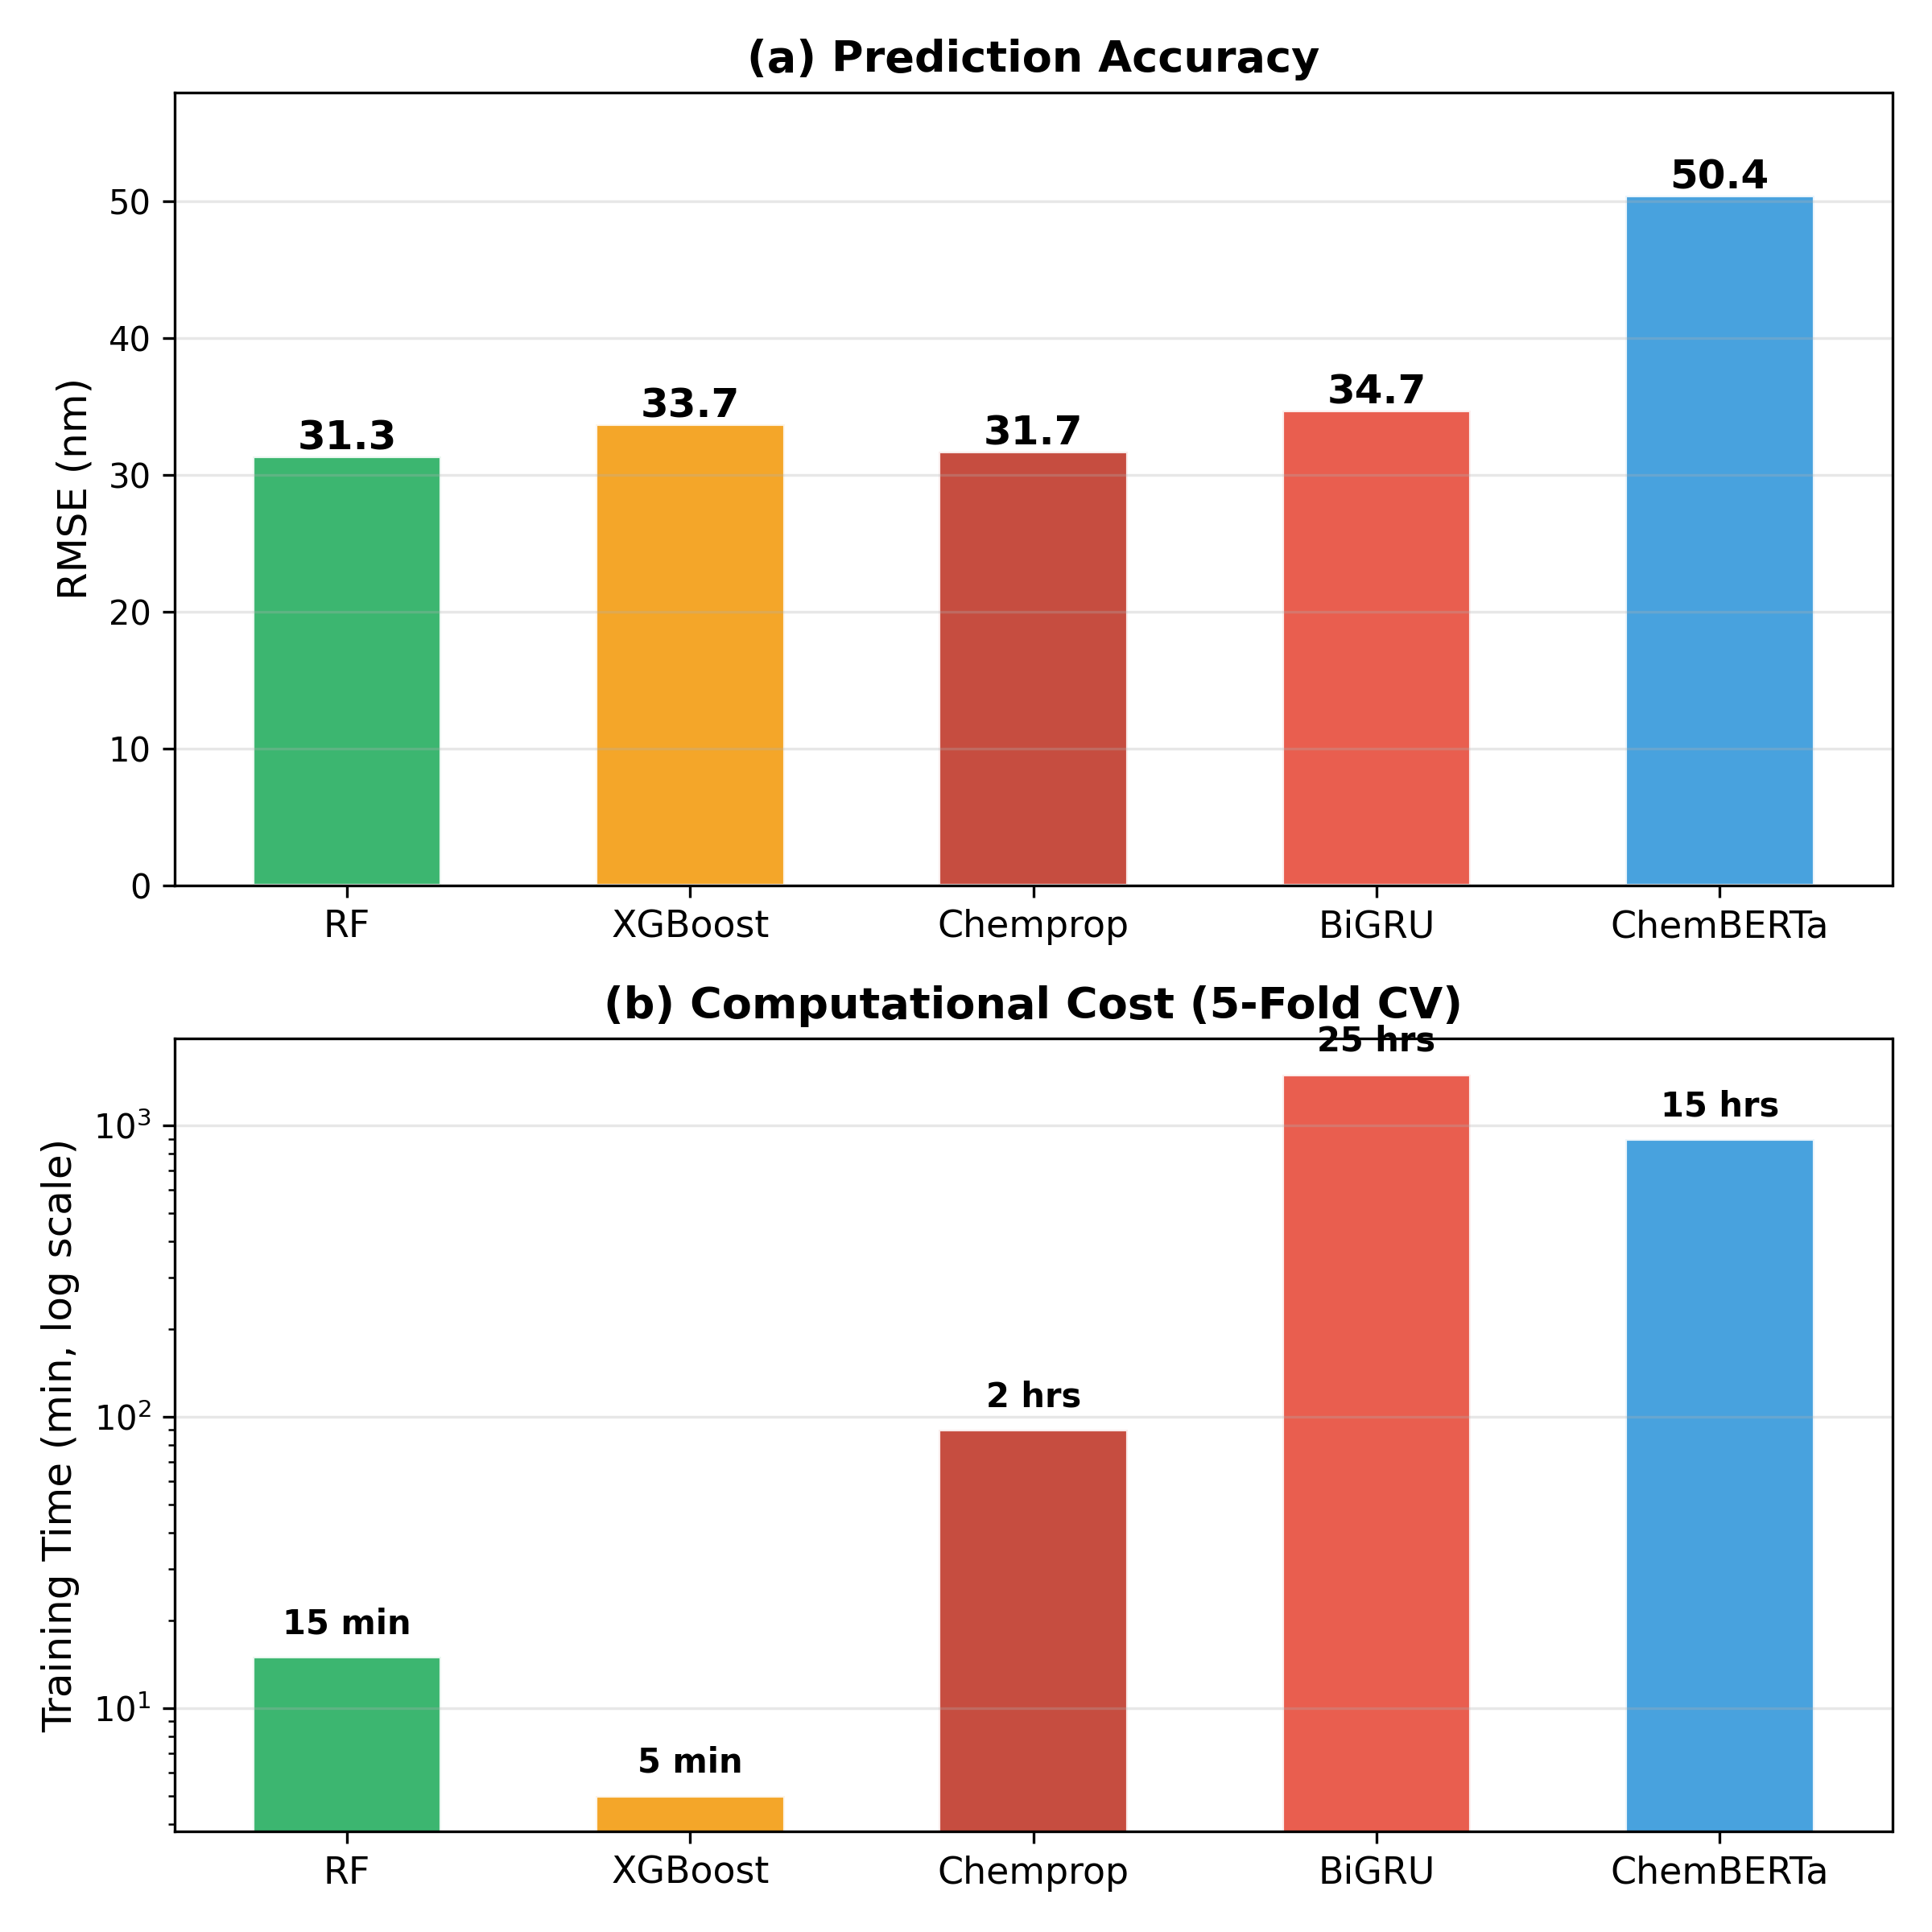
\includegraphics[width=0.65\textwidth]{results/rf_training_comparison.png}
    \caption{Training time vs.\ performance comparison. (a)~RF attains performance statistically tied with the best deep learning model in 15~minutes of total training compared to BiGRU's 25~hours (100$\times$ faster). (b)~Computational cost on log scale highlights the practical advantage of fingerprint-based models.}
    \label{fig:rf_practical}
\end{figure}

\textbf{Feature importance reveals known photochemistry.}
The most important feature (bit 463, Gini importance = 12.7\%) corresponds to aryl diazo/hydrazine substructures.
Molecules containing this substructure exhibit a mean $\lambda_{\max}$ of 543~nm compared to 401~nm without ($\Delta\lambda_{\max} = +143$~nm), consistent with the well-known bathochromic effect of nitrogen-nitrogen double bonds extending $\pi$-conjugation.
Other high-ranking features include BODIPY cores ($\Delta\lambda_{\max} = +162$~nm), enamine linkages ($\Delta\lambda_{\max} = +141$~nm), and alkynyl silane groups ($\Delta\lambda_{\max} = +153$~nm), all recognized chromophore motifs in photochemistry (Figure~\ref{fig:rf_interpretability}a).

\textbf{Solute dominates, solvent contributes modestly.}
Partitioning feature importance between solute and solvent fingerprint bits reveals that solute structure accounts for 96.1\% of total importance, with solvent contributing 3.9\% (Figure~\ref{fig:rf_interpretability}b).
This aligns with chemical intuition: chromophore structure is the primary determinant of $\lambda_{\max}$, while solvatochromic shifts are secondary effects.
The 24.6:1 solute-to-solvent importance ratio is consistent with the modest 6--8\% RMSE improvement observed in the solvent ablation.

\textbf{Model sparsity.}
Despite operating on 4096-dimensional fingerprint input, the RF model concentrates its decisions on a small subset of features: the top 5 features explain 26.9\% of total importance, the top 20 explain 41.6\%, and the top 100 explain 62.6\% (Figure~\ref{fig:rf_cumulative}).
A single fingerprint bit corresponding to aryl diazo/hydrazine substructures accounts for 12.7\% of total importance, reflecting the dominant contribution of azo chromophores to large $\lambda_{\max}$ values in the dataset ($\Delta\lambda = +143$~nm when present).

\textbf{Practical advantages of classical ML.}
Beyond interpretability, RF offers substantial practical advantages for molecular property prediction tasks.
RF training completes in approximately 15 minutes on a single CPU, compared to 1.5 hours for Chemprop and 25 hours for BiGRU on GPU, while achieving comparable or lower RMSE (Figure~\ref{fig:rf_practical}b).
RF requires no GPU hardware, no hyperparameter tuning of learning rates or batch sizes, and no early stopping strategy.
These results highlight that, depending on the dataset and molecular application domain, it is prudent to evaluate classical ML models where appropriate to gain insights into relative performance before directly deploying deep learning architectures.
While deep learning retains clear advantages in scenarios requiring transfer learning, end-to-end learning from raw data, or scalability to very large datasets, the simplicity, speed, and interpretability of fingerprint-based models make them a valuable complement, and in some cases a preferred alternative, in the molecular property prediction toolkit.

\textbf{Instance-level interpretability for BiGRU.}
While RF provides \emph{global} interpretability (which substructures matter dataset-wide), the BiGRU model offers complementary \emph{instance-level} interpretability.
Prior work has explored masking-based approaches for SMILES interpretability~\cite{gohSMILES2VecInterpretableGeneralPurpose2018}; here we explore gradient-based saliency analysis~\cite{simonyan2014deep}.
We computed Input$\times$Gradient saliency for each SMILES character position, then mapped character-level scores to atoms using RDKit's canonical SMILES atom-ordering~\cite{landrumRdkitRdkit2020_03_12020}, and visualized the resulting atom-level importance as 2D molecular heatmaps via SimilarityMaps~\cite{riniker2013similarity} (Figure~\ref{fig:bigru_saliency}).

The saliency maps reveal that BiGRU learns chemically meaningful patterns consistent with the RF feature importance analysis: high-saliency atoms concentrate on heteroatoms (O, N, S) and atoms adjacent to double bonds, the functional groups that determine $\pi$-conjugation and UV absorption wavelength, while aliphatic chains receive low saliency.
For molecules where BiGRU predicts accurately (e.g., Sinapic Acid, err = $-5.6$~nm), saliency is focused on the hydroxyl and methoxy groups of the chromophore; for poorly predicted molecules (e.g., Cinnamic Acid, err = $+78.2$~nm), the model over-attributes importance to the carboxylic acid rather than the conjugated vinyl bridge.
This convergence between RF's substructure-level Gini importance and BiGRU's atom-level gradient saliency provides independent confirmation that both models learn the same underlying photochemistry through fundamentally different architectures, a form of \emph{triangulation} that strengthens confidence in the learned structure--property relationships.
We note that gradient saliency identifies correlations rather than causal mechanisms, and that attention weights in Transformer-based models are even less reliable for interpretability~\cite{jain2019attention} (see Supporting Information, Figure~S4, for character-type importance analysis).

\begin{figure}[htbp]
    \centering
    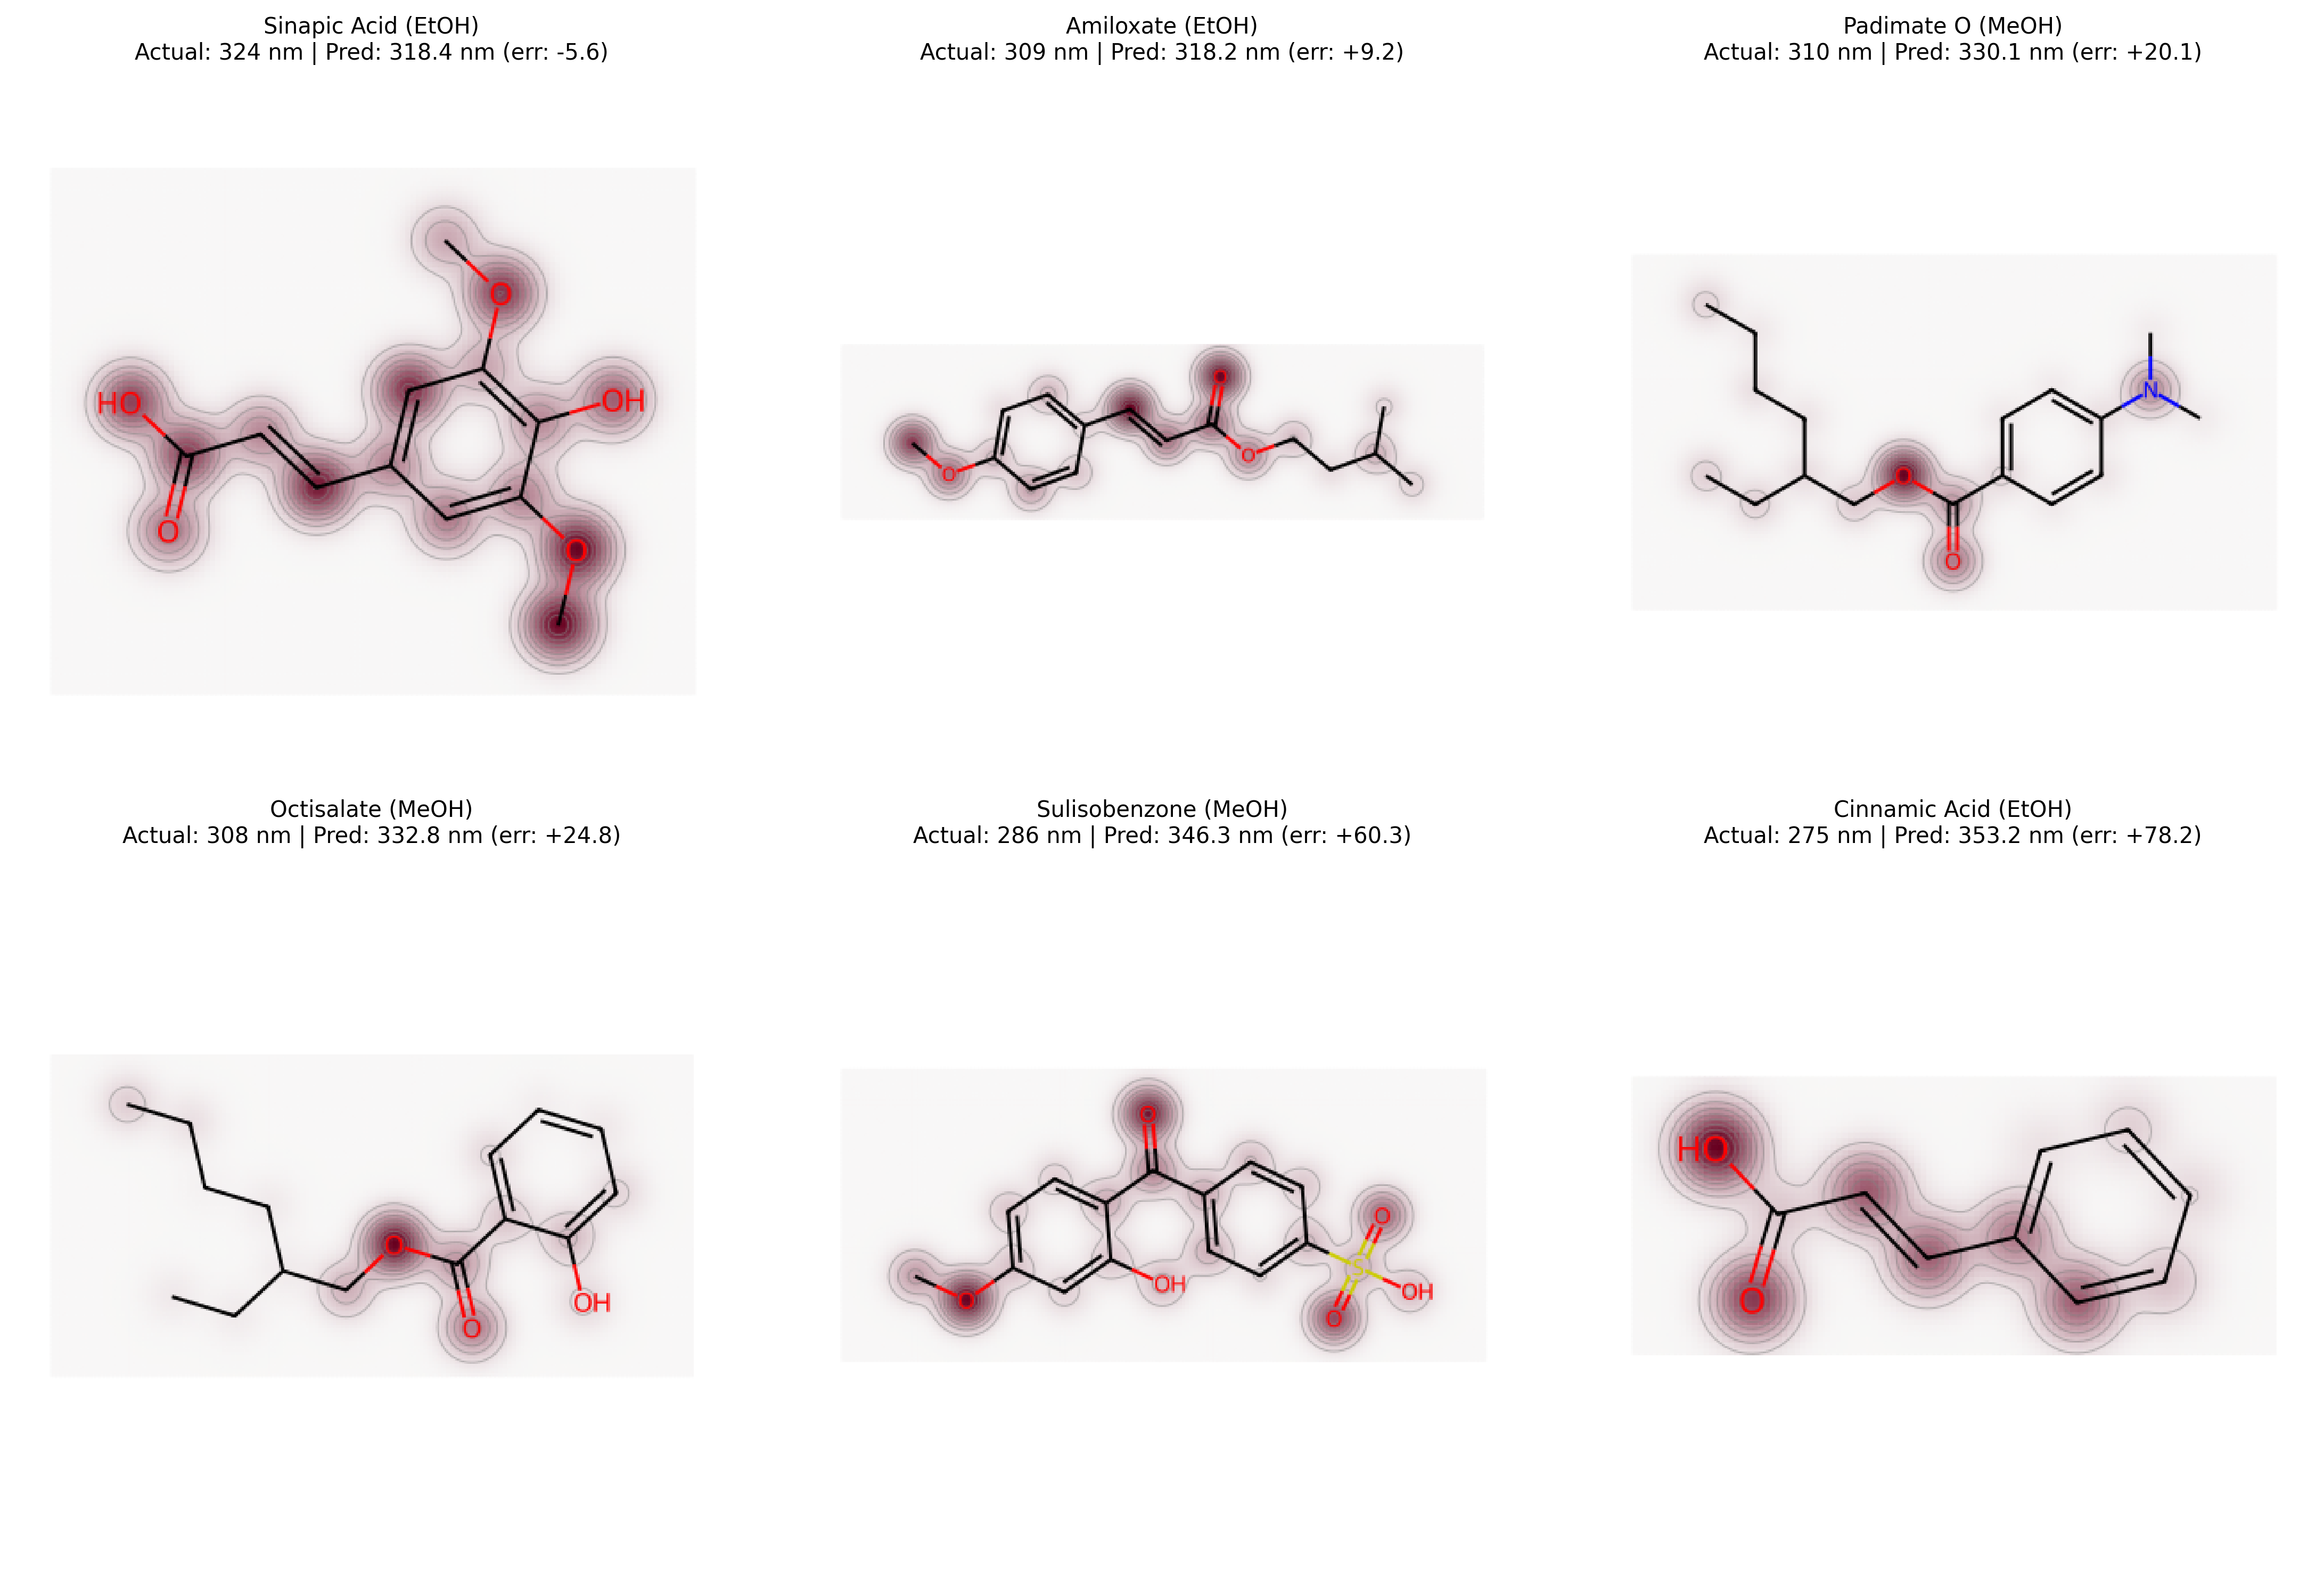
\includegraphics[width=\textwidth]{results/bigru_saliency_atoms.png}
    \caption{BiGRU gradient saliency mapped to 2D molecular structures for six wetlab validation molecules. Atom color intensity reflects gradient-based importance (red = high saliency). Top row: well-predicted molecules ($|\text{error}| < 22$~nm); bottom row: poorly predicted molecules ($|\text{error}| > 28$~nm). In both groups, heteroatoms (O, N) and atoms adjacent to double bonds receive the highest saliency, consistent with the character-type analysis (Figure~S4) where bond symbols (\texttt{=}, \texttt{\#}) and heteroatoms rank $2.5\text{--}3.5\times$ above aliphatic carbons. This overlap with the chromophore motifs identified by RF feature importance confirms that the BiGRU learns chemically meaningful attention patterns. Large prediction errors (e.g., Octocrylene +61~nm, Cinnamic Acid +81~nm) therefore arise not from misidentified features but from limitations in encoding extended conjugation length and specific solvent effects from 1D SMILES.}
    \label{fig:bigru_saliency}
\end{figure}


% --- Photosafety Classification ---
\subsection{Photosafety Classification}
\label{sec:classification}

To evaluate practical utility, we apply our models to ICH~S10~\cite{ICH2013S10} photosafety classification using the Mamede et al.~\cite{mamede2021machine} protocol.
Compounds with $\lambda_{\max} \in [290, 700]$~nm and molar extinction coefficient (MEC) $\geq 1000$ are classified as photoreactive (POS).
We reconstructed the Mamede/Reaxys dataset by querying Reaxys using the CAS registry numbers listed in the original study, recovering 93.6\% of the original 74,784 compounds.
The 6.4\% gap arises from deprecated CAS entries, compounds removed from current Reaxys builds, and structures that could not be resolved to valid SMILES representations.
We trained a separate RF classifier on this reconstructed data, and additionally trained the tuned BiGRU architecture (3-layer, 256-unit) as a direct binary classifier with sigmoid output and BCE loss on the same dataset and test split.

\begin{table}[htbp]
\centering
\caption{Photosafety classification performance. POS = $\lambda_{\max} \in [290,700]$ nm AND MEC $\geq$ 1000. $^\dagger$Published result on original Reaxys dataset; our models use a reconstructed version (93.6\% recovery) with a different test split, so comparison is approximate.}
\label{tab:classification}
\begin{tabular}{lccccc}
\toprule
\textbf{Model} & $\boldsymbol{N_{\text{test}}}$ & \textbf{Sensitivity} & \textbf{Specificity} & \textbf{Accuracy} & \textbf{AUC} \\
\midrule
Mamede RF (2021)$^\dagger$  & 998   & 0.90  & 0.88  & 0.89  & ---   \\
Our RF                      & 1,996 & 0.876 & 0.882 & 0.879 & 0.942 \\
BiGRU direct cls            & 1,996 & 0.794 & 0.811 & 0.803 & 0.886 \\
\bottomrule
\end{tabular}
\end{table}

Our RF classifier closely reproduces the published Mamede results (accuracy 0.879 vs.\ 0.89), validating both our Reaxys dataset reconstruction and the effectiveness of Morgan fingerprints for photosafety screening.
When the tuned BiGRU is trained as a direct binary classifier on the same data, it achieves accuracy 0.803, substantially below RF (0.879).
This gap reinforces the advantage of explicit substructure encoding (Morgan fingerprints) over character-level SMILES representations for classification tasks where specific functional-group presence determines the label.


% --- Experimental Validation ---
\subsection{Experimental Validation}
\label{sec:experimental}

To further validate our models, we measured UV absorption spectra for 16 commercially available compounds (Figure~\ref{fig:wetlab_molecules}) in both ethanol (EtOH) and methanol (MeOH), yielding 32 experimental $\lambda_{\max}$ values.
Of these 16 molecules, 15 are entirely absent from the training dataset, providing a genuine out-of-distribution test.
One molecule (Ferulic Acid) appears in the training data with a different solvent (water).
Although ethanol and methanol are well-represented solvents in the training set (1,034 and 1,322 records, respectively), the solute--solvent combinations tested here are novel.

\begin{figure}[htbp]
\centering
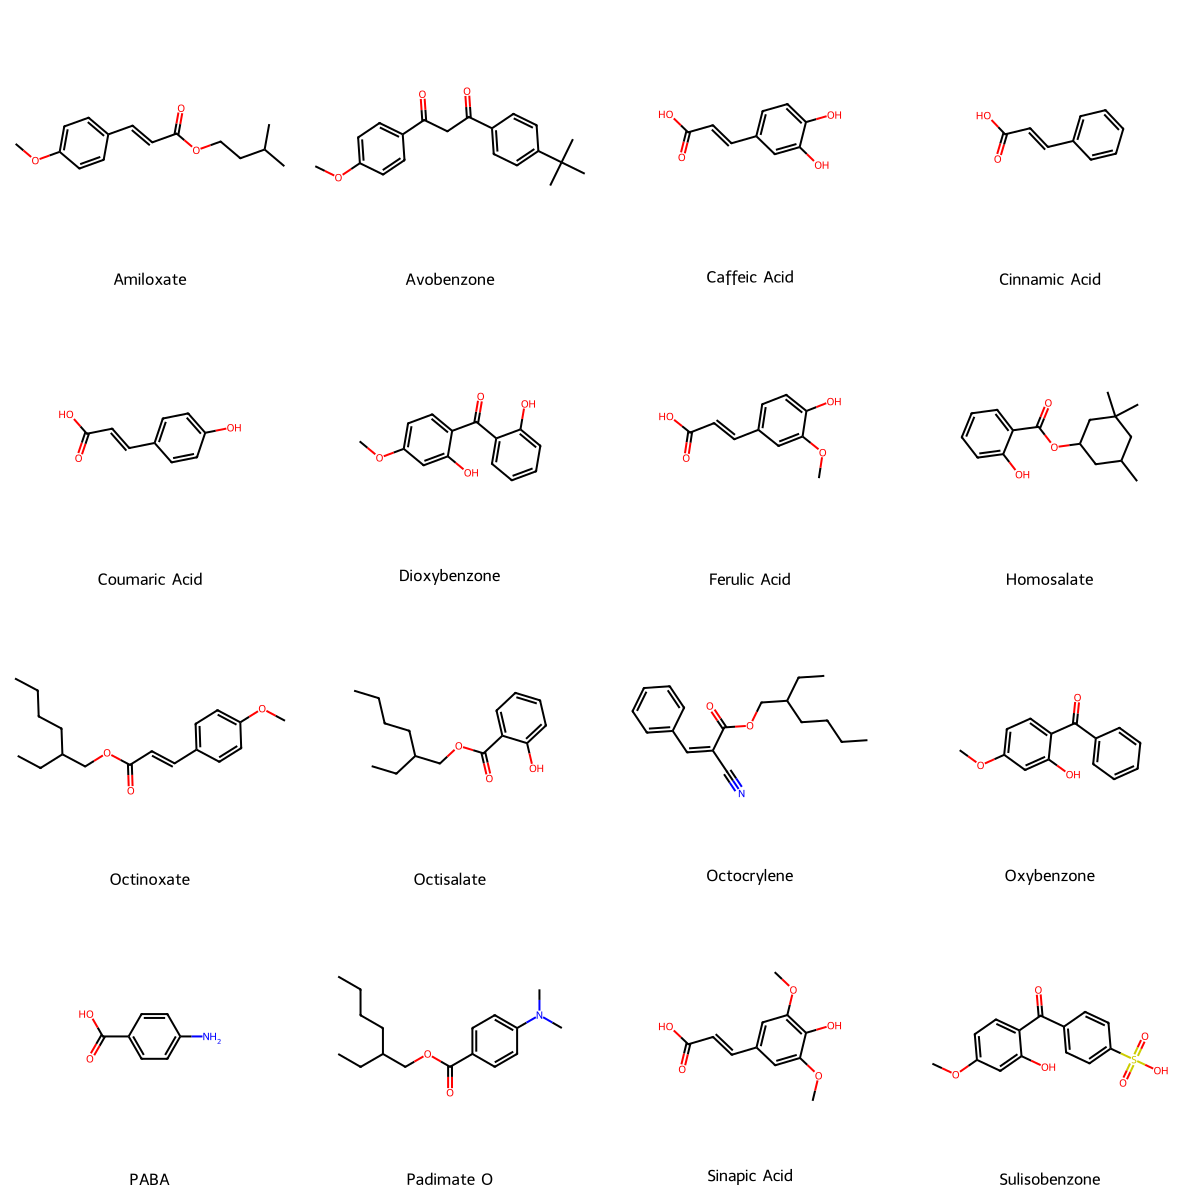
\includegraphics[width=\columnwidth]{results/wetlab_molecules.png}
\caption{Molecular structures of the 16 UV-absorbing compounds used for experimental validation. These commercially available sunscreen actives and phenolic acids span a range of chromophore classes (cinnamates, salicylates, benzophenones, aminobenzoates) with experimental $\lambda_{\max}$ values from 275 to 358~nm.}
\label{fig:wetlab_molecules}
\end{figure}

\begin{table}[htbp]
\centering
\caption{Experimental validation: predicted vs.\ measured $\lambda_{\max}$ (nm) for 16 UV-absorbing compounds in two solvents. GNN = D-MPNN, CB = ChemBERTa. Predictions are ensemble averages across 5-fold models. \colorbox{goodpred}{Green} cells indicate predictions within 10~nm of the experimental value. $^*$Present in training data with a different solvent.}
\label{tab:experimental}
\small
\begin{tabular}{lccccccccccc}
\toprule
& \multicolumn{5}{c}{\textbf{Ethanol}} & & \multicolumn{5}{c}{\textbf{Methanol}} \\
\cmidrule(lr){2-6} \cmidrule(lr){8-12}
\textbf{Molecule} & \textbf{Exp.} & \textbf{GNN} & \textbf{CB} & \textbf{BiGRU} & \textbf{RF} & & \textbf{Exp.} & \textbf{GNN} & \textbf{CB} & \textbf{BiGRU} & \textbf{RF} \\
\midrule
Amiloxate       & 309 & \gp{309} & 349 & \gp{318} & 359 & & 298 & \gp{302} & 347 & 316 & 359 \\
Avobenzone      & 358 & \gp{354} & 323 & 329 & 337 & & 358 & \gp{351} & 318 & 327 & 333 \\
Caffeic Acid    & 325 & \gp{319} & 342 & 338 & 347 & & 325 & 309 & \gp{335} & \gp{335} & 345 \\
Cinnamic Acid   & 275 & \gp{276} & 348 & 353 & 348 & & 276 & 265 & 341 & 351 & 345 \\
Coumaric Acid   & 310 & \gp{302} & 340 & 348 & 346 & & 309 & 294 & 333 & 343 & 344 \\
Dioxybenzone    & 283 & 367 & 314 & 315 & 327 & & 283 & 359 & 308 & 315 & 320 \\
Ferulic Acid$^*$  & 324 & 311 & \gp{326} & 313 & 346 & & 324 & 302 & \gp{321} & 310 & 344 \\
Homosalate      & 308 & 336 & 295 & 335 & 332 & & 308 & 335 & 293 & 336 & 327 \\
Octinoxate      & 309 & 328 & 325 & 326 & 334 & & 308 & 322 & 323 & 323 & 332 \\
Octisalate      & 308 & 334 & 291 & 339 & 353 & & 308 & 333 & 291 & 333 & 349 \\
Octocrylene     & 301 & 385 & 357 & 344 & 390 & & 302 & 381 & 350 & 344 & 389 \\
Oxybenzone      & 287 & 334 & 325 & \gp{301} & 328 & & 287 & 327 & 317 & \gp{299} & 321 \\
PABA            & 291 & \gp{282} & \gp{295} & 322 & 308 & & 290 & 279 & \gp{294} & 319 & 306 \\
Padimate O      & 310 & 325 & \gp{320} & 334 & 340 & & 310 & 324 & \gp{316} & 330 & 337 \\
Sinapic Acid    & 324 & 312 & 343 & \gp{318} & 347 & & 324 & 303 & \gp{332} & \gp{314} & 346 \\
Sulisobenzone   & 287 & 338 & 330 & 346 & 355 & & 286 & 334 & 326 & 346 & 352 \\
\midrule
\textbf{MAE (nm)} & & \textbf{25.5} & 27.8 & 28.9 & 39.3 & & & \textbf{26.9} & 24.9 & 28.4 & 37.7 \\
\textbf{RMSE (nm)} & & 36.5 & \textbf{33.5} & 34.4 & 44.4 & & & 34.8 & \textbf{30.8} & 33.4 & 43.0 \\
\bottomrule
\end{tabular}
\end{table}

\begin{table}[htbp]
\centering
\caption{Aggregate wetlab validation metrics (16 molecules $\times$ 2 solvents = 32 data points). 95\% bootstrap CIs from 10,000 resamples.}
\label{tab:wetlab_summary}
\begin{tabular}{lcc}
\toprule
\textbf{Model} & \textbf{MAE (nm) [95\% CI]} & \textbf{RMSE (nm) [95\% CI]} \\
\midrule
Chemprop (D-MPNN) & \textbf{26.2}              & 35.7 \\
ChemBERTa         & 26.3 [20.1--33.0] & \textbf{32.2} [25.2--38.8] \\
BiGRU (default)   & 28.6 [22.7--35.0] & 33.9 [26.2--41.2] \\
BiGRU (tuned)     & 31.5 & 37.0 \\
RF + Morgan FP    & 38.5 [31.6--45.9]          & 43.7 [35.3--51.7] \\
\bottomrule
\end{tabular}
\end{table}

Chemprop (GNN), ChemBERTa (CB-Transformer), and BiGRU all outperform RF on this experimental validation set. Averaging across both solvents (32 predictions), Chemprop achieves the lowest MAE (26.2~nm), followed closely by ChemBERTa (26.3~nm [95\% bootstrap CI: 20.1--33.0]), BiGRU (28.6~nm [22.7--35.0]), and RF (38.5~nm [31.6--45.9]).
ChemBERTa achieves the lowest RMSE (32.2~nm) because Chemprop has several large outlier errors on benzophenone derivatives (Dioxybenzone, Oxybenzone: 40--84~nm errors), inflating its RMSE (35.7~nm) despite competitive median accuracy.
On cross-validated benchmarks, ChemBERTa was worst (RMSE = 50.39~nm) and Chemprop was tied with RF; yet on novel compounds, deep learning models consistently outperform RF.
This gap reflects a fundamental difference: RF relies on exact substructure matching through Morgan fingerprint bits, excelling at interpolation within the training distribution but struggling when novel functional groups or conjugation patterns are underrepresented.
The deep learning models, by contrast, learn representations (Chemprop from molecular graphs, BiGRU from sequential SMILES patterns, ChemBERTa from pretrained molecular language understanding) that can generalize to unseen molecular motifs.
All models show substantially higher errors than their cross-validated performance (ChemBERTa: 26.3 vs.\ 24.3~nm MAE; BiGRU default: 28.6 vs.\ 20.7~nm; RF: 38.5 vs.\ 15.2~nm), confirming that these 16 compounds are genuinely challenging out-of-distribution examples.
The tuned BiGRU (3L/256u) performs \textit{worse} on wetlab validation (MAE = 31.5~nm) than the default (28.6~nm), despite 4.8\% lower cross-validated RMSE. This is a bias--variance tradeoff: the larger architecture overfits to in-distribution patterns at the cost of out-of-distribution generalization.

Cinnamic Acid (experimental $\lambda_{\max}$ = 275--276~nm) is a notable outlier: ChemBERTa, BiGRU, and RF all overpredict by $\sim$65--78~nm, though Chemprop handles it well (1--11~nm error).
The experimental peak lies at the edge of the 270--400~nm scan range, suggesting measurement limitations.
Octocrylene is particularly problematic for RF (error $\sim$89~nm) and Chemprop ($\sim$81~nm), vs.\ 43~nm for BiGRU and 52~nm for ChemBERTa, likely because its extended cyano-acrylate conjugation is underrepresented in the training data.

All three models capture the small solvent sensitivity between EtOH and MeOH (typically 0--1~nm experimentally), though with some overestimation of the solvent shift magnitude (average predicted shifts of 2.5~nm for BiGRU, 2.9~nm for RF, and 4.9~nm for ChemBERTa).

These results show that RF is the preferred choice for screening within known chemical space (e.g., virtual screening of compound libraries with well-represented scaffolds), while deep learning models (BiGRU and ChemBERTa) are better suited for exploring novel molecular architectures where the training distribution may not cover all relevant substructures.
This data-dependent model selection finding is consistent with the observations of Chen et al.~\cite{chenMolecularLanguage2023}, who found that RNNs outperform Transformers on local-feature-dependent molecular generation tasks.
Our cross-validated results suggest that a similar architectural trade-off may apply in property prediction: since UV absorption depends on local chromophore features, models that capture local patterns (RF with fingerprints, BiGRU processing SMILES subsequences) achieve the best in-distribution performance.
ChemBERTa's weak cross-validated performance but strong wetlab generalization suggests that pretrained representations may encode transferable molecular knowledge that compensates for the architecture's inductive bias mismatch, but only when evaluated on truly novel compounds outside the training distribution.
This complementarity extends beyond the local/global distinction: RF's fixed-vocabulary substructure matching excels at interpolation, while learned representations (both BiGRU and ChemBERTa) enable extrapolation to novel scaffolds.

\begin{figure}[htbp]
    \centering
    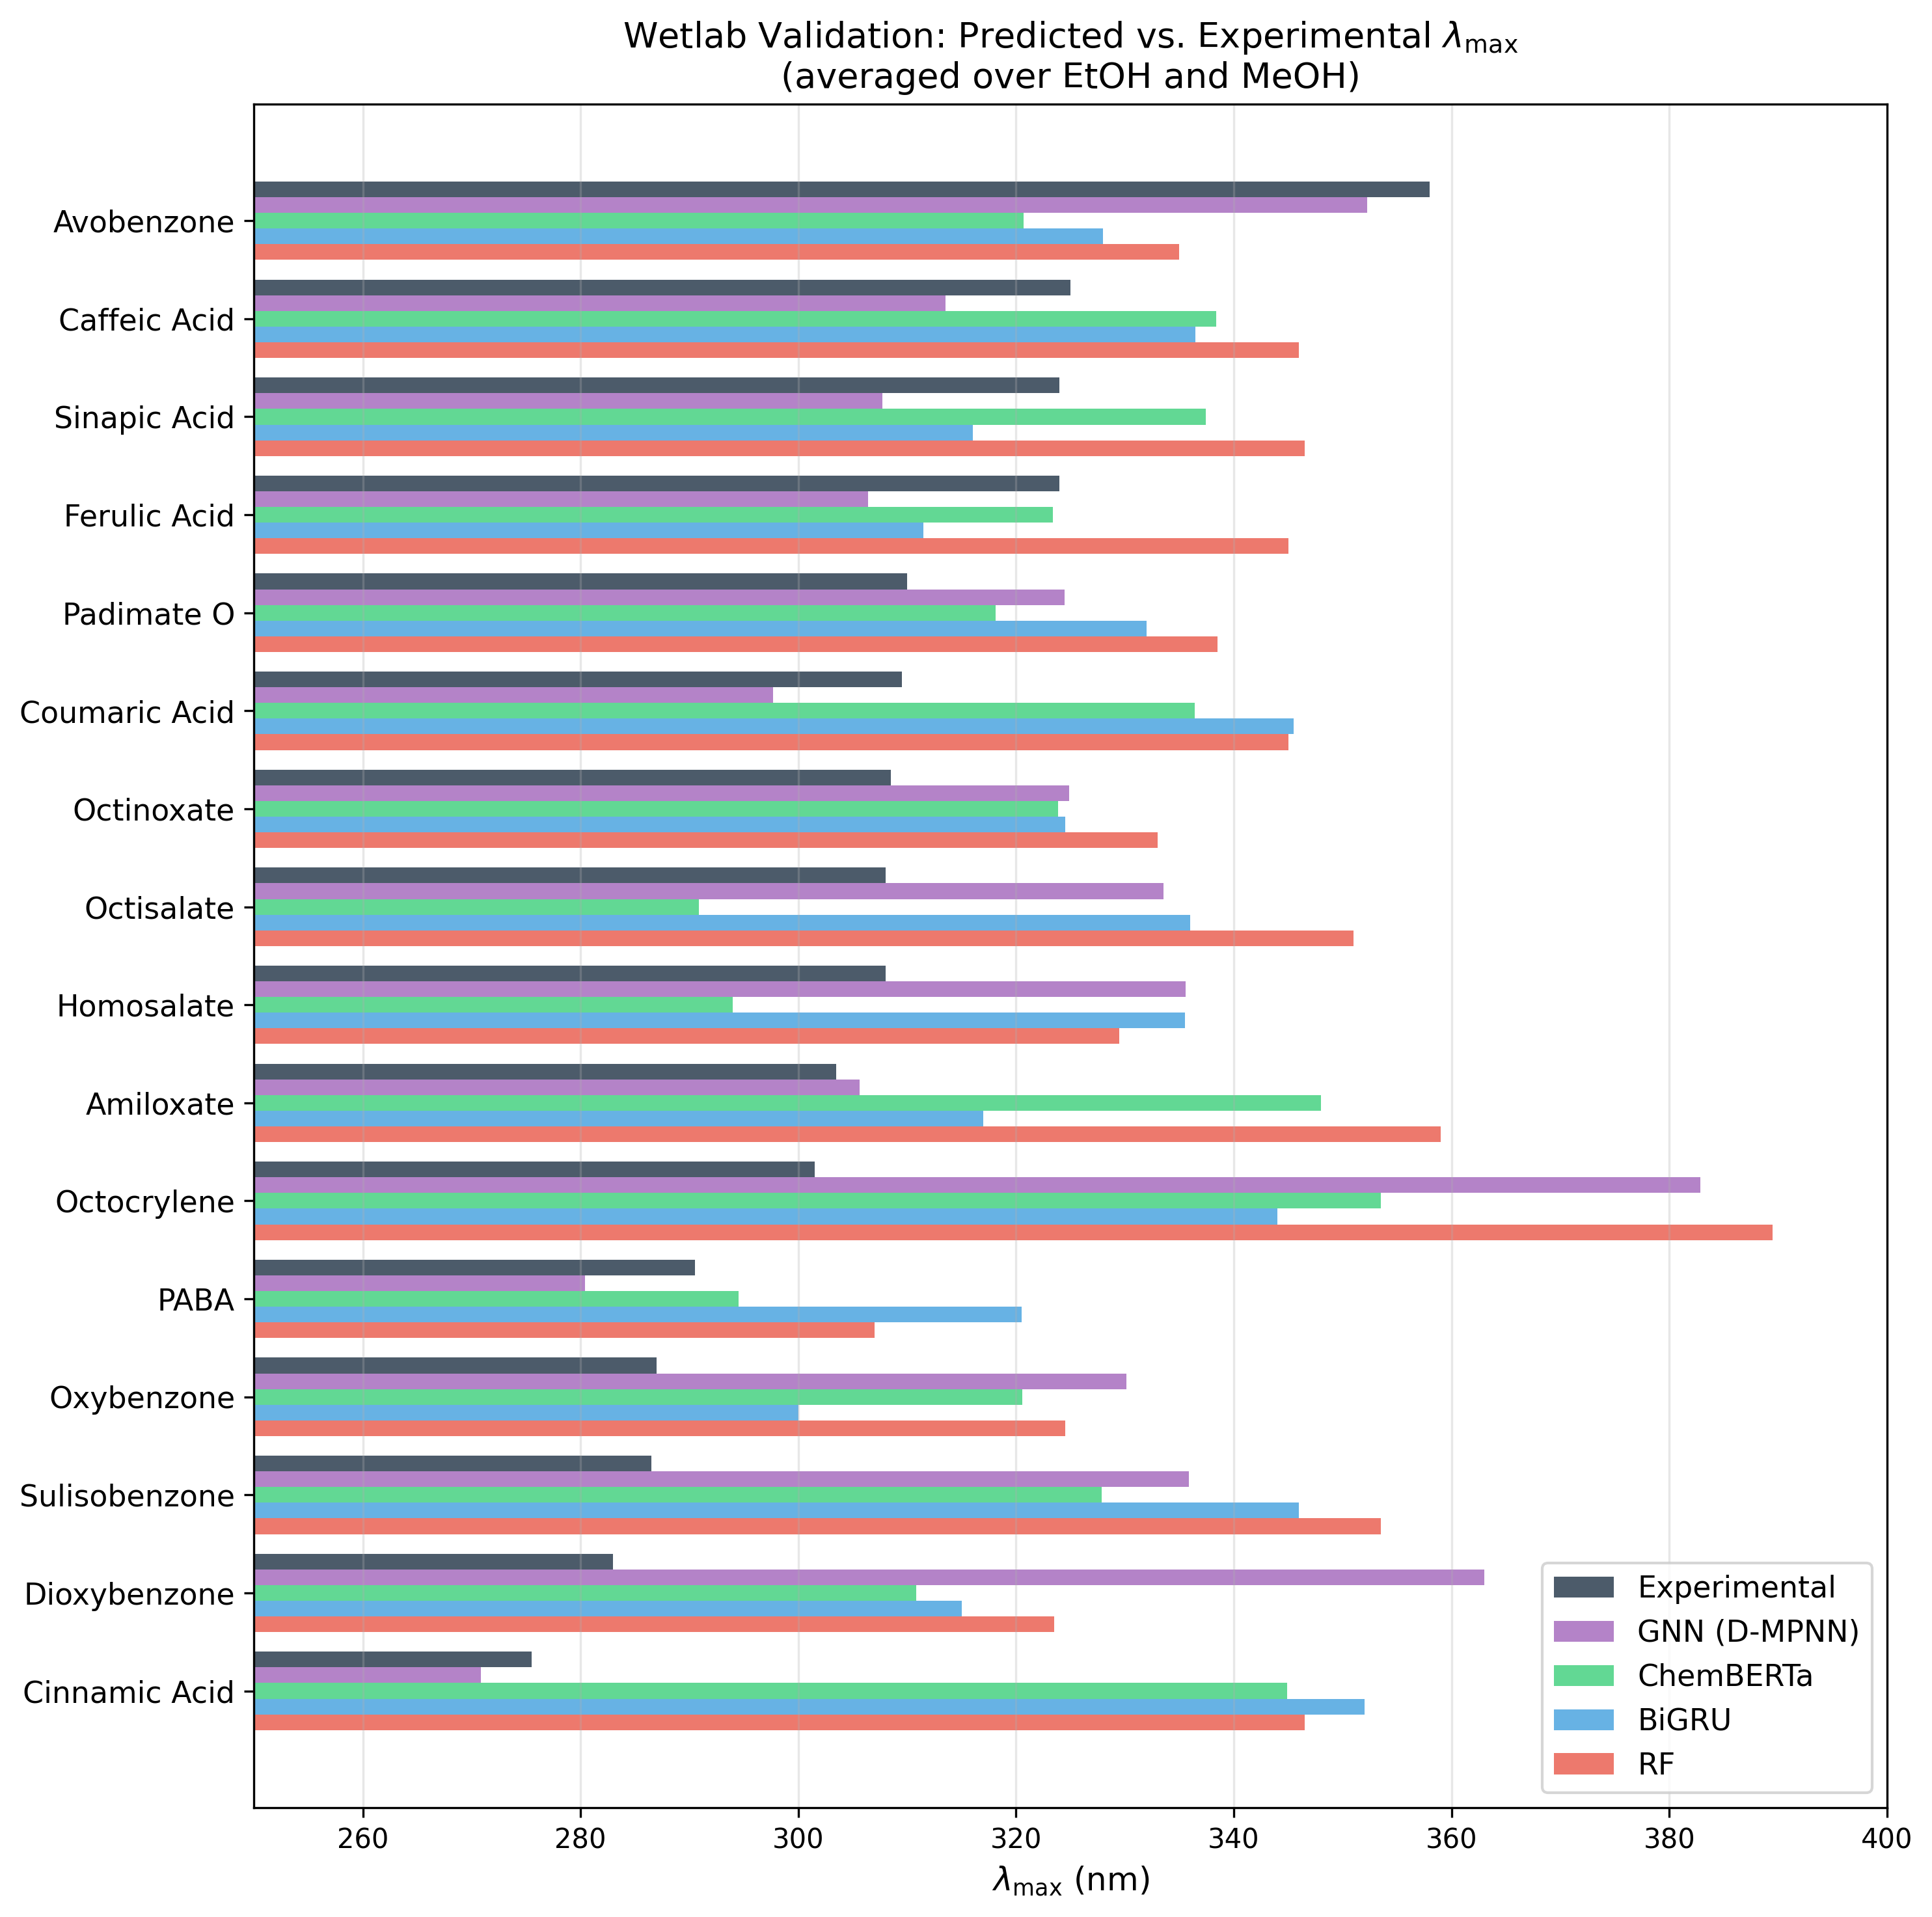
\includegraphics[width=\textwidth]{results/wetlab_per_molecule.png}
    \caption{Per-molecule comparison of experimental and predicted $\lambda_{\max}$ for 16 sunscreen-related compounds, averaged over EtOH and MeOH solvents. Molecules are sorted by experimental $\lambda_{\max}$. The D-MPNN closely tracks experimental values for small chromophores (Cinnamic Acid, PABA) but overpredicts benzophenones (Dioxybenzone, Octocrylene), while all models struggle with Octocrylene.}
    \label{fig:wetlab_per_molecule}
\end{figure}

Figure~\ref{fig:wetlab_per_molecule} shows per-molecule predictions alongside experimental values, illustrating the pattern more concretely: the D-MPNN achieves near-exact predictions for Cinnamic Acid and PABA where other models overpredict by 60--80~nm, while all models struggle with Octocrylene. ChemBERTa tracks the experimental trend most closely for mid-range absorbers (Padimate~O, Ferulic Acid).

% ===== Conclusion =====
\section{Conclusion}
\label{sec:conclusion}

We have presented a systematic benchmark of ML approaches for UV absorption wavelength prediction, comparing Random Forest, XGBoost, Chemprop (D-MPNN), BiGRU, and ChemBERTa across three datasets totaling over 60,000 molecules.

Our key findings are:

\begin{enumerate}
    \item \textbf{RF and deep learning have complementary strengths.}
    RF with Morgan fingerprints and the Chemprop D-MPNN achieve statistically indistinguishable cross-validated performance on the primary Joung+Beard dataset (RMSE = 31.34 and 31.69~nm, $p = 0.77$), both outperforming the tuned BiGRU (34.71~nm) and ChemBERTa (50.39~nm). Chemprop surpasses published baselines on both external datasets: Deep4Chem (RMSE = 19.13 vs.\ GCNN 26.6~nm~\cite{joung2021deep}) and Jung 2024 (RMSE = 27.36 vs.\ Multifidelity 31.3~nm), with RF close behind (22.70 and 29.82~nm respectively).
    However, on 16 experimentally validated novel compounds, all deep learning models (Chemprop MAE = 26.2~nm, ChemBERTa 26.3~nm, BiGRU 28.6~nm) outperform RF (38.5~nm), demonstrating that learned representations generalize to out-of-distribution molecules where fixed fingerprints fall short.
    This indicates that RF excels at interpolation within known chemical space, while learned representations (from graphs, sequences, or pretraining) generalize beyond fixed substructural features.

    \item \textbf{Solvent encoding improves all model families.}
    Encoding solute and solvent as a single concatenated representation reduces RMSE by 6--8\% across all tested architectures (RF 8\%, Chemprop 6\%, BiGRU 7\%; all $p < 0.02$).
    This simple approach requires no domain-specific descriptor engineering and is applicable to any model that accepts molecular representations.

    \item \textbf{Both model families offer interpretability.}
    RF provides global interpretability through feature importance: the top 20 Morgan fingerprint bits (out of 4096) explain over 41\% of importance and map to known chromophore motifs (aryl diazo, BODIPY, enamine).
    BiGRU, optimized via Bayesian HPO (3-layer, 256-unit architecture, 4.8\% RMSE improvement over the default on 5-fold CV), provides instance-level interpretability through gradient saliency analysis, with atom-level heatmaps highlighting the same conjugated regions identified by RF.
    RF trains 100$\times$ faster (15 minutes CPU vs.\ 25 hours GPU), making it the practical first choice when the target chemical space is well-represented in training data, while BiGRU's learned representations offer better generalization to novel scaffolds.

    \item \textbf{Practical classification favors fingerprint models.}
    RF-based photosafety classification (accuracy = 0.879) closely reproduces the published Mamede benchmark (accuracy = 0.89), while BiGRU direct classification reaches only 0.803, confirming that Morgan fingerprints' explicit substructure encoding is superior for binary photosafety screening.
\end{enumerate}

Our results raise a testable hypothesis about model selection: that architectures whose inductive bias matches the locality of the target property will outperform global-attention architectures in-distribution, while pretrained representations confer out-of-distribution advantages regardless of inductive bias. The present work establishes this pattern for UV absorption $\lambda_{\max}$; whether it extends to fluorescence emission, lipophilicity, aqueous solubility, or other molecular endpoints whose locality differs from UV absorption requires dedicated cross-property benchmarking, which we identify as a priority for future work.

\subsection*{Limitations}
Our models use 1D or 2D molecular representations (fingerprints, SMILES, molecular graphs); 3D conformational information may become important for structurally diverse chromophores where electronic properties depend on molecular geometry~\cite{lupopasini2023excited}.
Solvents are encoded purely through their molecular structure (SMILES or fingerprints), without explicit physical properties such as dielectric constant, refractive index, or Hansen solubility parameters~\cite{reichardt2011solvents}, which may limit the models' ability to capture fine-grained solvatochromic effects.
The BiGRU model uses character-level tokenization, which may miss chemically meaningful substructures; ChemBERTa's BPE tokenizer partially addresses this but still operates on 1D SMILES strings.
The experimental validation set (16 molecules) is small; larger out-of-distribution evaluations would strengthen the generalization finding, though the consistent advantage of deep learning on novel compounds is robust.
Bayesian hyperparameter optimization of BiGRU (25 Optuna trials, extended to 5-fold CV) reduced its cross-validated RMSE by 4.8\% (from 36.45 to $34.71 \pm 1.40$~nm), narrowing but not closing the gap with RF (31.34~nm); however, ChemBERTa hyperparameters remain untuned due to prohibitive training cost.
ChemBERTa's 44.1M parameters may also be overparameterized for the $\sim$12K training samples available per fold.
While tuning substantially mitigates the asymmetry concern for BiGRU, the remaining 10\% performance gap supports the hypothesis that fingerprint representations have an inherent advantage for in-distribution UV absorption prediction.
Furthermore, the tuned BiGRU shows \textit{worse} out-of-distribution performance on wetlab validation (MAE = 31.5~nm vs.\ 28.6~nm for the default), suggesting that the larger architecture overfits to training distribution patterns.
Finally, the Wilcoxon signed-rank test (a non-parametric alternative appropriate for small samples) yields $p = 0.0625$ for all model comparisons due to the minimum achievable $p$-value with $n = 5$ concordant pairs; larger-scale cross-validation (e.g., 10-fold) would provide stronger non-parametric statistical power.

\subsection*{Future Work}
Transfer learning from larger UV absorption databases (e.g., the Reaxys dataset of $\sim$70K records) may improve BiGRU performance and narrow the gap with RF on cross-validated benchmarks, exploiting deep learning's capacity for pretraining~\cite{vermeire2021transfer}, an advantage that classical ML cannot replicate.
Incorporating 3D structural information through hybrid architectures~\cite{gilmer2017neural} or precomputed quantum-chemical descriptors~\cite{lupopasini2023excited} could improve predictions for geometry-dependent chromophores.
Ensemble approaches combining RF and BiGRU predictions could use RF's interpolation accuracy for well-represented scaffolds and BiGRU's extrapolation capability for novel structures.
We have demonstrated instance-level interpretability for BiGRU through gradient saliency analysis; extending gradient-based methods (rather than unreliable attention weights~\cite{jain2019attention}) to ChemBERTa and other Transformer architectures is a natural next step.
More broadly, our in-distribution results are consistent with the hypothesis that architecture choice in molecular ML may be influenced by the locality of the target property~\cite{chenMolecularLanguage2023, jiang2023trangru}: properties determined by local substructures (UV absorption, functional group-dependent activity) favor fingerprint and RNN-based approaches on cross-validated benchmarks, while out-of-distribution evaluation reveals that additional factors such as pretraining data and learned representations can overcome architectural mismatch.
A natural extension is to apply the same benchmarking framework to related molecular optical properties, including fluorescence emission wavelength, molar extinction coefficient ($\varepsilon$), and lipophilicity, to determine whether the patterns observed here generalize across property types or whether properties with different structure--property relationships (e.g., global vs.\ local determinants) shift the balance between model families.


% ===== Data and Code Availability =====
\section*{Data and Code Availability}
The primary Joung+Beard dataset and the Deep4Chem database are available from the same Figshare repository~\cite{joung2020experimental, beard2019comparative} (DOI: 10.6084/m9.figshare.12045567).
Additional external dataset: Jung et al.\ (GitHub)~\cite{jung2024machine}.
The Mamede classification dataset was reconstructed from Reaxys~\cite{mamede2021machine}.
All code for model training, evaluation, and analysis will be released on GitHub under the MIT license upon publication, including trained model weights and preprocessing scripts.


% ===== Acknowledgement =====
\begin{acknowledgement}
The authors thank the University of Iowa and the Midwest Bioprocessing Center for computational resources.
This research did not receive any specific grant from funding agencies in the public, commercial, or not-for-profit sectors.
Claude Opus 4.6 (Anthropic) was used to assist with code debugging, code review, and manuscript formatting; all scientific content, analysis, and interpretation are solely the work of the authors.
\end{acknowledgement}

The authors declare no competing financial interest.

% ===== Supporting Information =====
\begin{suppinfo}
The Supporting Information is available free of charge at [DOI].

Per-fold cross-validation results for all five model families including solvent ablation (Tables~S1--S7), statistical significance tests (Table~S8), RF hyperparameter sensitivity analysis, BiGRU and ChemBERTa learning curves (Figures~S1--S2), hyperparameter tuning asymmetry analysis (Table~S9), Joung+Beard vs.\ Deep4Chem overlap analysis (Figure~S3), and BiGRU character-type saliency analysis (Figure~S4) (PDF).
\end{suppinfo}

% ===== Bibliography =====
\bibliography{Proposal}

\end{document}
